\documentclass[mat1]{fmfdelo}
% \documentclass[fin1]{fmfdelo}
% \documentclass[isrm1]{fmfdelo}
% \documentclass[mat2]{fmfdelo}
% \documentclass[fin2]{fmfdelo}
% \documentclass[isrm2]{fmfdelo}

% naslednje ukaze ustrezno napolnite
\avtor{Izak Jenko}

% \naslov{Kompleksni torusi in eliptične krivulje}
\naslov{Eliptične krivulje in kompleksni torusi}
% \title{Complex tori and elliptic curves}
\title{Elliptic curves and complex tori}

% navedite ime mentorja s polnim nazivom: doc.~dr.~Ime Priimek,
% izr.~prof.~dr.~Ime Priimek, prof.~dr.~Ime Priimek
% uporabite le tisti ukaz/ukaze, ki je/so za vas ustrezni
\mentor{izr.~prof.~dr.~Sašo Strle}
% \mentorica{}
% \somentor{}
% \somentorica{}
% \mentorja{}{}
% \mentorici{}{}

\letnica{2022} % leto diplome

%  V povzetku na kratko opišite vsebinske rezultate dela. Sem ne sodi razlaga organizacije dela --
%  v katerem poglavju/razdelku je kaj, pač pa le opis vsebine.
\povzetek{\emph{Eliptična krivulja} nad poljem kompleksnih števil $\C$ je nesingularna projektivna kubika, podana z Weierstrassovo enačbo. S pomočjo izreka o implicitni funkciji pokažemo, da ta dopušča kompleksno sturkturo, kar pomeni, da postane Riemannova ploskev. Po drugi strani vsak torus, predstavljen kot kvocient $\C$ po mreži $\Lambda$ -- diskretni podgrupi $\C$ izomorfni $\Z^2$, podeduje kompleksno strukturo preko kvocientne preslikave in tako upraviči imenovanje \emph{kompleksni torusi}. Izkaže se, da ti dve, bistveno različni konstrukciji, presenetljivo porodita enaka \oz izomorfna matematična objekta. To vez razložimo preko teorije dvojno periodičnih funkcij, imenovanih eliptične funkcije, in modularnih funkcij z mnogo simetrije povezane z modularno grupo $\operatorname{SL}_2(\Z)$. Obravnavamo njihove osnovne lastnosti in razijemo teorijo Weierstrassove funkcije $\wp$, ki nam nazadnje omogoči eksplicitno podati omenjeni izomorfizem in dokazati uniformizacijski izrek, ki združuje oba objekta.
} 

%  Prevod slovenskega povzetka v angleščino.
\abstract{An \emph{elliptic curve} over the field of complex numbers $\C$ is a nonsingular projective cubic, given by the Weierstrass equation. Using the implicit function theorem we show, that it admits a complex structure, which makes it a Riemann surface. 
On the other hand every torus, which we view as a quotient of $\C$ modulo a lattice $\Lambda$ -- a discrete subgroup of $\C$ isomorphic to $\Z^2$, inherits a complex structure via its quotient map and justifies us naming them \emph{complex tori}. These two, vastly different construcions, remarkably trun out to yield the same i.~e.\ isomorphic mathematical objects. This link is explaind using the theory of doubly periodic functions, also called elliptic functions, and modular functions, which are meromorphic functions on the upper half plane enjoying many symmetries involving the modular group $\operatorname{SL}_2(\Z)$. 
We discuss their basic properties and develop the necessary theory of the Weierstrass $\wp$-function, alowing us to explicitly construct the aforementioned isomorphism and prove the uniformizaton theorem, unifying both objects of study. 

% can be endowed with a complex stru 

% \[
%     y^2z = 4x^3 - axz^2 - bz^3, \quad \text{with } a^3 -27b^2 \neq 0.    
% \]
% In this paper we expose a remarkable link between elliptic curves and complex tori, which we view as quotiens of $\C$ modulo a lattice and poses a natural complex structure. 
%  which allows us to view them as Riemann surfaces.  
}

% navedite vsaj eno klasifikacijsko oznako --
% dostopne so na www.ams.org/mathscinet/msc/msc2020.html
\klasifikacija{11F03, 11G05, 14H52, 14H55}
\kljucnebesede{eliptična krivulja, eliptična funkcija, kompleksni torus, Weierstrassova funkcija $\wp$, $j$-invarianta, modularna funkcija} % navedite nekaj ključnih pojmov, ki nastopajo v delu
\keywords{elliptic curve, elliptic function, complex torus, Weierstrass $\wp$-function, $j$-invariant, modular function} % angleški prevod ključnih besed

\zapisiMetaPodatke  % poskrbi za metapodatke in veljaven PDF/A-1b standard

% aktivirajte pakete, ki jih potrebujete
% \usepackage{tikz}
\usepackage{bm}
\usepackage{array}
% \usepackage[dvipsnames]{xcolor}
% \usepackage[usenames,dvipsnames]{color}
\usepackage{faktor}
\usepackage{caption}
\usepackage{xfrac}
\usepackage[shortlabels]{enumitem}
\usepackage{tikz-cd}
\usepackage{quiver}
\usepackage{mathrsfs}
% \usepackage{physics}
\usepackage{graphicx}
\graphicspath{ {./images/} }

%%%

\usepackage{amsmath}
\usepackage{array}
\usepackage{tikz}
\usetikzlibrary{decorations.pathreplacing}
\newcommand{\tikzmark}[1]{\tikz[overlay,remember picture,baseline=(#1.base)]
\node (#1) {\strut};}

%%%  
\usetikzlibrary{decorations.markings}
\usetikzlibrary{cd, babel}

\numberwithin{equation}{section}

\newcommand{\R}{\mathbb R}
\newcommand{\N}{\mathbb N}
\newcommand{\Z}{\mathbb Z}
\newcommand{\C}{\mathbb C}
\newcommand{\HH}{\mathfrak{H}}
\newcommand{\PP}{\mathbb P}
\newcommand{\Lattice}{\mathscr{L}}
\newcommand{\CM}{\mathbb C ^*}
% \newcommand{\PC}{P^2(\mathbb C)}
\newcommand{\PC}{\mathbb{P}^2_\C}
\newcommand{\Q}{\mathbb Q}
\newcommand{\RS}{\widehat{\C}}
\newcommand{\Cxyz}{\C[x,y,z]}
\newcommand{\linphi}{\mathcal{A}_\Phi}
\newcommand{\oio}{\pcoor{0: 1 : 0}}
\newcommand{\om}{\omega}
\newcommand{\inv}{^{-1}}
\newcommand{\torus}{\C/\Lambda}
\newcommand{\elf}{\C(\Lambda)}
% \newcommand{\SL}{\operatorname{SL}_2(\Z)}
\newcommand{\SL}{\Gamma}

\newcommand{\abcd}{\big(\begin{smallmatrix} a & b\\c & d \end{smallmatrix}\big)}
\newcommand{\pabcd}{\begin{pmatrix} a & b \\ c & d \end{pmatrix}}

\newcommand{\iso}{\cong}
\newcommand{\homeo}{\approx}
\newcommand{\htp}{\simeq}

\newcommand{\pcoor}[1]{%
\begingroup\lccode`~=`: \lowercase{\endgroup
\edef~}{\mathbin{\mathchar\the\mathcode`:}\nobreak}%
\left[% opening symbol
\begingroup
\mathcode`:=\string"8000
#1%
\endgroup
\right]% closing symbol
}

\newcommand{\pdv}[2][]{\frac{\partial#1}{\partial#2}}

\newcommand{\bigslant}[2]{{\raisebox{.2em}{$#1$}\left/\raisebox{-.2em}{$#2$}\right.}}

% \newcommand{\res}[2]{\operatorname{res}_{#1}\left(#2\right)}
% \newcommand{\ord}[2]{\operatorname{ord}_{#1}\left(#2\right)}

\newcommand{\res}[2]{\operatorname{res}_{#1}(#2)}
\newcommand{\ord}[2]{\operatorname{ord}_{#1}(#2)}

\newcommand{\hol}[1]{\mathcal{O}(#1)}

\newcommand{\abs}[1]{\left\lvert #1 \right\rvert}

\newcommand{\disk}[2]{\Delta(#1, #2)}

\newcommand{\lattice}[2]{\left\langle #1, #2 \right\rangle}

% \newcommand{\Im}[1]{\operatorname{Im}\left(#1\right)}
\AtBeginDocument{%
  \renewcommand\Re{\operatorname{Re}}%
}

\AtBeginDocument{%
  \renewcommand\Im{\operatorname{Im}}%
}

%command for alg-closure that automatically adapts its 'bar' to the arg based on the args length (including '\')
\newcommand{\ols}[1]{\mskip.5\thinmuskip\overline{\mskip-.5\thinmuskip {#1} \mskip-.5\thinmuskip}\mskip.5\thinmuskip} % overline short
\newcommand{\olsi}[1]{\,\overline{\!{#1}}} % overline short italic

\newcommand{\ti}{t.~i.\ }
\newcommand{\tj}{tj.\ }
\newcommand{\oz}{oz.\ }

% stari komentar, ki ne dela, ker uporablja xcolor
% \newcommand{\kom}[1]{
%     \textcolor{Blue}{//#1}
% }

\newcommand{\kom}[1]{
    \underline{//#1}
}


% matematične operatorje deklarirajte kot take, da jih bo Latex pravilno stavil
% \DeclareMathOperator{\conv}{conv}

\DeclareMathOperator{\GL}{GL}
\DeclareMathOperator{\Aut}{Aut}
\DeclareMathOperator{\rang}{rang}
\DeclareMathOperator{\id}{id}
\DeclareMathOperator{\pr}{pr}

% vstavite svoje definicije ...
%  \newcommand{}{}

\theoremstyle{definition}
\newenvironment{komentar}[1][Komentar]{\begin{proof}[#1]\let\qed\relax}{\end{proof}}

\definecolor{material-theme}{HTML}{263238}
\definecolor{material-theme-palenight}{HTML}{292D3E}

\begin{document}

% začasna menjava barv v pdf-ju, da bo lažje za gledat ponoči
% \pagecolor{material-theme-palenight}
% \color{white}

%--------------------------------------------------------------------------%
%%%%%%%%%%%%%%%%%%%%%%%%%%%%%% 1. UVOD %%%%%%%%%%%%%%%%%%%%%%%%%%%%%%%%%%%%%
%--------------------------------------------------------------------------%

\section{Uvod}

Matematike pogosto zanimajo rešitve različnih enačb. Obstoj rešitev, kakšne lastnosti imajo in
kako se obnašajo pod raznimi transformacijami. Osrednja tema moje naloge bo preučiti in ustvariti
geometrijsko predstavo množice ničel kompleksnega polinoma tretje stopnje posebne oblike. 
To množico ničel si lahko predstavljamo kot realno ploskev in ji pravimo eliptična krivulja.   
Zgodovinsko je eliptična krivulja množica ničel enačbe
\[
    y^2 = x^3 + ax + b. 
\]
V tem delu pa se bomo ukvarjali z nekoliko prilagojeno -- projektivno -- obliko te enačbe. Množicam ničel
polinomov več spremenljivk pravimo \emph{algebraične krivulje} in z njimi bomo začeli v poglavju \ref{algebraicne krivulje}. 
\par 
Pri iskanju rešitev
polinomskih enačb se razmeroma hitro porodi vprašanje, iz katerega ambientnega prostora 
sploh sprejemamo veljavne rešitve. Spomnimo se fundametalnega izreka algebre, ki pravi, da ima
vsak nekonstanten polinom s kompleksnimi koeficienti ničlo v polju kompleksnih števil, med tem
ko brez težav poiščemo realne polinome, ki realnih ničel nimajo. Podobno situacijo imamo tukaj. 
Eliptične krivulje se namreč da študirati nad mnogo različnimi polji. Nad končnimi polji igrajo
eliptične kriulje pomembno vlogo v kriptografiji, nad poljem racionalnih števil in njihovimi končnimi razširitvami -- številskimi polji -- pridejo do izraza v algebraični teoriji
števil, mi pa jih bomo v tem delu gledali nad poljem kompleksnih števil. 
\par
V primeru obravnave nad poljem kompleksnih števil eliptične
krivulje naravno pridobijo dodatno kompleksno stukturo in na ta način postanejo \ti \emph{Riemannove ploskve}. Ta struktura nam omogoči analizo holomorfnih funkcij na prostorih, ki niso nujno domene v kompleksni ravnini in jo
bomo bolj podrobno preiskali v poglavju \ref{riemannove ploskve}.
Po drugi strani bomo toruse vpeljali kot kvocientne prostore kompleksne ravnine $\C$ po delovanju diskretne grupe izomorfne $\Z^2$. To delovanje bo na nek način dovolj regularno, da bo tako konstruirani kvocientni prostor prevzel ključne lokalne lastnosti kompleksne ravnine in nam tako olajšal definicijo kompleksne strukture in interpretacije holomorfnih funkcij na njem. Skupaj s to strukturo bomo ta kvocientni prostor imenovali kompleksni torus in izkazal se bo za najbolj primerno domeno \ti \emph{eliptičnih funkcij}. V osnovi so eliptične \oz dvojno periodične funkcije meromorfne funkcije z dvema periodama -- v dveh realno linearno neodvisnih smereh v kompleksni ravnini. Njihove lastnosti in obnašanje si bomo ogledali v poglavju \ref{elipticne funkcije}, ključno vlogo pa bo igrala prav posebna Weierstrassova eliptična funkcija $\wp$.
% Ta pogled bo precej poenostavil definicijo kompleksne strukture in interpretacije holomorfnih funkcij na njem
% V nadaljevanju bomo videli, da tudi torus premore strukturo Riemannove ploskve in ga bomo skupaj s to strukturo imenovali kompleksni torus. Izkaže se, da je kompleksni
% torus najbolj smiselna domena dvojno periodičnih oz. eliptičnih funkcij. Lastnosti in obnašanje eliptičnih funkcij si bomo ogledali v poglavju \ref{elipticne funkcije}, ključno vlogo pa bo igrala prav posebna Weierstrassova eliptična funkcija $\wp$.
Skupaj s svojim kompleksnim odvodom Weierstrassova funkcija $\wp$ zadošča enačbi
\[
  \wp'(z)^2 = 4\wp(z)^3 - g_2\wp(z) - g_3,  
\] 
ki je po obliki presenetljivo podobna enačbi eliptične krivulje. Idejo, da je domena eliptične funkcije lahko kompleksni torus, na tem primeru interpretiramo kot dejstvo, da kompleksni torus in par funkcij $(\wp, \wp')$ parametrizira eliptično krivuljo podano z enačbo $y^2 = 4x^3 - g_2x - g_3$.
% Z nadaljevanjem analogije o eliptičnih funkcijah kot preslikeve na kompleksnem torusu, vidimo, da nek določen torus 
Ta zveza nam bo nazadnje v poglavju \ref{poglavje izomorfizem} omogočila konstrukcijo preslikave, ki bo pokazala, da sta kompleksni torus in eliptična krivulja v nekem smislu enaka matematična objekta. Vsakemu kompleksnemu torusu bo tako pripadala neka eliptična krivulja, s pomočjo \emph{modularnih funkcij} pa bomo pokazali še obrat, kako iz eliptične krivulje priti nazaj do kompleksnega torusa. 
\\

Vredno je še opomniti, da eliptične krivulje in področja, v katerih se uporabljajo,
nimajo več vsebinsko praktično nič opravka z elipsami. 
Izkazalo se je, da so inverzi funkcij, s katermi računamo dolžine lokov elips, dvojno periodični,
če jih gledamo kot funkcije kompleksne spremenljivke in od tod pride ime eliptičnih funkcij. V teh izračunih namreč integriramo izraze oblike $R(t, \sqrt{f(t)})$, kjer je $R \in \C(x,y)$ racionalna funkcija in $f$ polinom tretje ali četrte stopnje brez kvadratnih faktorjev. Ravno polinom $f$, pa se pod ustrezno uvedbo nove spremenljivke da transformirati v desno stran enačbe, ki podaja eliptično krivuljo. 
% Pri tem pa polinom $f$ usteza ravno desni strani enačbe, ki podaja podaja eliptično krivuljo. 
% Te dvojno periodične funkcije pa so tesno povezane z enačbo,
% ki ji zadoščajo eliptične krivulje in se bomo k njim vrnili v poglavju \ref{elipticne funkcije}.

%--------------------------------------------------------------------------%
%%%%%%%%%%%%%%%%%%%%%% 2. ALGEBRAIČNE KRIVULJE %%%%%%%%%%%%%%%%%%%%%%%%%%%%%
%--------------------------------------------------------------------------%

\section{Algebraične krivulje} \label{algebraicne krivulje}
Algebraične krivulje so množice ničel polinomov nad različnimi polji. V tem poglavju bomo začeli 
z afinimi
algebraičnimi krivuljami, ki jih v nadaljevanju sicer ne bomo direktno potrebovali, bodo pa igrale pomembno
vlogo pri razumevanju projektivnih algebraičnih krivulj, ki jih bomo vpeljali takoj za tem. 
Zaradi namenov tega dela, algebraičnih krivulj ne bomo obravnavali nad povsem splošnimi polji, pač pa se
bomo omejili na polje kompleksnih števil, ki ga bomo označevali s $\C$. V smislu enodimenzionalnega kompleksnega prostora bomo množici kompleksnih števil pravili tudi kompleksna premica.

%%%%% Afine algebraične krivulje %%%%%

\subsection{Afine algebraične krivulje} 
Naj $\C[x_1, \dots, x_n]$ označuje kolobar polinomov $n$ spremenljivk s
kompleksnimi koeficienti. Množica ničel poljubnega polinoma $f \in \C[x_1, \dots, x_n]$ je
\[
    V(f) = \{p \in \C^n \mid f(p) = 0 \} \subseteq \C^n.
\] 

\begin{definicija}
    Množica $C \subseteq \C^2$ je \emph{afina algebraična krivulja}, če obstaja tak nekonstanten polinom $f \in \C[x,y]$, da je
    \[
        C = V(f).
    \]
\end{definicija}

Afine algebraične krivulje si lahko predstavljamo, kot nekaj podobnega ploskvam v prostoru $\R^4$, če naredimo identifikacijo $\C \equiv \R^2$. Dve kompleksni spremenljivki polinoma lahko zamenjamo s štirimi realnimi, prav tako pa tedaj tudi polinomska enačba $f(x,y) = 0$ razpade na dve realni. To sta
\[
    \Re f(x_1 + ix_2, y_1 + iy_2) = 0 \quad \text{in} \quad \Im f(x_1 + ix_2, y_1 + iy_2) = 0,
\]
kjer so $x_1, x_2, y_1, y_2 \in \R$ realne spremenljivke.
Pogoji, ki jim zadoščajo točke na afini algebraični krivulji $C \subseteq \R^4$, so zelo podobni tistim, ki definirajo gladke pod\-mnogoterosti z glavno razliko, da gradienti teh definicijskih funkcij niso nujno (realno) linearno neodvisni. To bi bilo na $C$ razvidno kot samopresečišča ali osti, ki pa jih podmnogoterosti seveda nimajo. 
\par
V ta namen bi radi definirali singularne točke na afini algebraični krivulji $C = V(f)$ kot rešitve sistema enačb 
\[ 
    \pdv[f]{x}(x_0, y_0) = 0, \quad \pdv[f]{y}(x_0, y_0) = 0, \quad f(x_0, y_0) = 0.
\]
Toda ta definicija zaenkrat ni dobra, saj polinom $f \in \C[x,y]$ ni enolično določen s krivuljo $C$. 
Zato uvedemo pojem minimalnega polinoma krivulje $C$.

\begin{definicija}
    Naj bo $C$ afina algebraična krivulja. \emph{Minimalni polinom} krivulje $C$ je polinom $f \in C[x,y]$ najmanjše stopnje, za katerega velja $V(f) = C$.
\end{definicija}
% V definiciji, bi radi uporabili polinom $f \in \C[x,y]$, katerega množica ničel je krivulja $C$, toda ta poliom s krivuljo ni enolično določen zato najprej uvedimo pojem minimalnega polinoma krivulje $C$.

\begin{opomba}
    Če je $f$ minimalni polinom krivulje $C$, je to tudi $\alpha f$ za $\alpha \in \CM$, saj je $V(f) = V(\alpha f)$. Minimalni polinomi afine algebraične krivulje se tako lahko razlikujejo za neničelno konstanto.
\end{opomba}

S pomočjo minimalnega polinoma krivulje, lahko sedaj definiramo singularne in regularne točke na njej.

\begin{definicija}
    \label{reg sing tocke}
    Naj bo $C$ afina algebraična krivulja in $f \in \C[x,y]$ njen minimalni polinom. Točka $(x_0, y_0) \in C$ je \emph{regularna}, če velja
    \[
        \frac{\partial f}{\partial x}(x_0, y_0) \neq 0 \quad \text{ ali } \quad \frac{\partial f}{\partial y}(x_0, y_0) \neq 0,
    \] 
    in \emph{singularna} sicer. Pravimo, da je afina algebraična krivulja \emph{singularna}, če vsebuje kakšno singularno točko, in je \emph{nesingularna} sicer.
\end{definicija}

\begin{primer*}
    Naj bo $f = x^2 + y^2 - 1$ in $g = (x^2 + y^2 - 1)^2$. Jasno je $V(f) = V(g)$, kar pomeni, da $f$ in $g$ določata isto algebraično krivuljo. Toda sistem 
    \begin{equation}
        \label{sistem f}
        \pdv[f]{x}(x,y) = 2x = 0, \quad \pdv[f]{y}(x,y) = 2y = 0, \quad f(x,y) = 0
    \end{equation}
    nima nobene rešitve, sistem
    \begin{align}
        \label{sistem g}
        \pdv[g]{x}(x,y) = 4x(x^2 + y^2 - 1) &= 0, \nonumber \\ 
        \pdv[g]{y}(x,y) = 4y(x^2 + y^2 - 1) &= 0, \\
        g(x,y) &= 0 \nonumber
    \end{align}
    pa jih ima veliko. Namreč vsaka rešitev enačbe $f(x,y) = x^2 + y^2 - 1 = 0$ reši sistem \eqref{sistem g}, od koder bi lahko napačno sklepali, da je vsaka točka krivulje $V(f)$ singularna. Minimalni polinom opazovane krivulje je $f$ in iz sistema \eqref{sistem f} vidimo, da singularnih točk nimamo, torej je krivulja nesingularna. 
    
\end{primer*}

Definicija \ref{reg sing tocke} nam omogoči formulirati prvo opazko.

\begin{trditev}
    Vsaka nesingularna afina algebraična krivulja $C \subseteq \C^2$ je z identifikacijo $\C^2 \equiv \R^4$ gladka $2$-podmnogoterost oz. ploskev.
\end{trditev}

\begin{dokaz}
    Najprej se spomnimo definicije podmnogoterosti. Neprazna podmnožica $X \subseteq \R^{n+k}$ je \emph{$n$-podmnogoterost} razreda gladkosti $\mathcal{C}^r$, za $r \in \{0,1,\dots, \infty, \omega\}$, če za vsako točko $x_0 \in X$ obstaja okolica $U \subseteq \R^{n+k}$ točke $x_0$ in t.~i.\ definicijska funkcija $F: U \subseteq \R^{n+k} \to \R^k$ razreda $\mathcal{C}^r$ na $U$, da velja
    \begin{enumerate}
        \item $X \cap U = F^{-1}(\{0\}) = \{x \in U \mid F(x) = 0\}$ in
        \item Jacobijeva matrika definicijske funkcije $F$ ima poln rang povsod na $X \cap U$, tj. $\rang J F(x) = k$ za vsak $x \in X \cap U$.
    \end{enumerate}
    Številu $n$ pravimo \emph{dimenzija} podmnogoterosti $X$, številu $k$ pa \emph{kodimenzija}.
    \\
    \par
    Sedaj poglejmo, da je pri nesingularnih afinih krivuljah tej definiciji zadoščeno. Definicijsko funkcijo imamo tokrat podano kar globalno na celotnem $\R^4$. Njeno vlogo igra minimalni polinom $f \in \C[x,y]$, ki podaja krivuljo $C = V(f)$. Polinom $f$ namesto kot funkcijo dveh kompleksnih spremenljivk interpretiramo kot funkcijo štirih realnih spremenljivk, njeno kodomeno, ki je $\C$, pa identificiramo z $\R^2$, tako da ločimo realni in imaginarni del funkcije $f(x_1 + ix_2, y_1 + iy_2) = u(x_1,x_2,y_1,y_2) + iv(x_1,x_2,y_1,y_2)$. Naj bo torej $g: \R^4 \to \R^2$ podana s predpisom
    \[
        g(x_1,x_2,y_1,y_2) = (u(x_1,x_2,y_1,y_2), v(x_1,x_2,y_1,y_2)).
    \]
    Jacobijeva matrika te preslikave je
    \[
    Jg = 
    \begin{pmatrix}
        u_{x_1} & u_{x_2} & u_{y_1} & u_{y_2} \\
        v_{x_1} & v_{x_2} & v_{y_1} & v_{y_2}
    \end{pmatrix}
    =
    \begin{pmatrix}
        u_{x_1} & -v_{x_1} & u_{y_1} & -v_{y_1} \\
        v_{x_1} & u_{x_1} & v_{y_1} & u_{y_1}
    \end{pmatrix},
    \]
    % \left (
    %     \begin{array}{rrrr}
    %         u_{x_1} & -v_{x_1} & u_{y_1} & -v_{y_1} \\
    %         \tikzmark{lower1} v_{x_1} & u_{x_1}\tikzmark{lower2} & \tikzmark{lower3} v_{y_1} & u_{y_1} \tikzmark{lower4}\\
    %     \end{array}
    % \right ),
    % \]
        
    % \begin{tikzpicture}[overlay, remember picture,decoration={brace,amplitude=5pt}]
    %     \draw[decorate,thick] (lower2.south) -- (lower1.south)
    %     node [midway,below=5pt] {$\pdv[f]{x}$};
    %     \draw[decorate,thick] (lower4.south) -- (lower3.south)
    %     node [midway,below=5pt] {$\pdv[f]{y}$};
    % \end{tikzpicture}
    % \newline
    % \newline
    % % $$
    % Jg = 
    % \begin{pmatrix}
    %     u_{x_1} & u_{x_2} & u_{y_1} & u_{y_2} \\
    %     v_{x_1} & v_{x_2} & v_{y_1} & v_{y_2}
    % \end{pmatrix}
    % =
    % \begin{pmatrix}
    %     u_{x_1} & -v_{x_1} & u_{y_1} & -v_{y_1} \\
    %     v_{x_1} & u_{x_1} & v_{y_1} & u_{y_1}
    % \end{pmatrix},
    % $$
    \noindent kjer smo v drugi enakosti po $2 \times 2$ blokih upoštevali Cauchy-Riemannov sistem enačb, saj imamo opravka s polinomi, ki so kot funkcije holomorfni v obeh svojih kompleksnih spremenljivkah. Izračun
    \[
        \pdv[f]{x} = \frac{1}{2} \left( \pdv[f]{x_1} - i\pdv[f]{x_2}\right) = \frac{1}{2} \left( u_{x_1} + i v_{x_1} - i u_{x_2} + v_{x_2}\right) = u_{x_1} + iv_{x_1},
    \]
    skupaj z analognim računom za $\pdv[f]{y} = u_{y_1} + iv_{y_1}$, in predpostavko o nesingularnosti krivulje nam zagotovita, da je v vsaki točki na $C$ vsaj eno od števil $u_{x_1} + iv_{x_1}$ in $u_{y_1} + iv_{y_1}$ neničelno. Normi teh dveh števil sta ravno determinanti levega \oz desnega $2\times 2$ bloka matrike $Jg$, ki ima zato v vsaki točki iz $C$ poln rang.
    % vsaj eden od parcialnih odvodov $u_{x_1}$, $v_{x_1}$, $u_{y_1}$, $v_{y_1}$ različen od $0$. Vsaj eden izmed levega \oz desnega $2\times 2$ bloka matrike $Jg$ 
    % To pa že zadošča za polnost ranga Jacobijeve matrike $Jg$ v dani točki, 
    % saj sta leva in desna $2 \times 2$ bloka alternativna predstavitev kompleksnih števil kot matrična algebra znotraj realnih $2 \times2$ matrik $M_2(\R)$.  
\end{dokaz}

Ta trditev pove, katere od afinih algebraičnih krivulj ne le lokalno v okolici regularnih točk izgledajo kot ploskve, temveč tudi so zares ploskve. 
\\
\par
Na tem mestu se pojavi manjša nejasnost, zakaj afine algebraične krivulje poimenovati ravno \emph{krivulje}. V kontekstu realnih podmnogoterosti se sprva to poimenovanje res zdi malce neusklajeno, toda v okviru kompleksnih dimenzij ta terminologija postane smiselna. Če v definiciji podmnogoterosti namreč zgolj zamenjamo polje realnih števil s $\C$, se povedano bistveno ne spremeni. Še vedno ohranimo dejstvo, da število ``linearno neodvisnih'' enačb ustreza kodimenziji podmnogoterosti in analogno tudi dimenzija podmnogoterosti ustreza razliki (kompleksne) dimenzije ambientnega prostora in kodimenzije. V tem smislu so potem ti objekti, ki jih realno vidimo kot ploskve, zares tudi kompleksne $1$-podmnogoterosti oziroma krivulje.

% \begin{opomba}
% Poimenovati te objekte ravno krivulje, se morda v tem kontekstu na prvi pogled zdi malce neusklajeno z našo predstavo iz realnih evlidskih prostorov. Toda, ker jih obravnavamo v smislu kompleksnih dimenzij 
% \end{opomba}
 
%%%%% Projektivne algebraične krivulje %%%%%

\subsection{Projektivne algebraične krivulje}

V tem razdelku bomo algebraične krivulje obravnavali še v projektivnem smislu. Definirali bomo kompleksno projektivno ravnino in krivulje v njej. Vpeljavo projektivne ravnine opravičujemo z mnogimi lepimi lastnostmi v povezavi s presečišči krivulj v njej, pa tudi z raznimi bolj topološkimi razlogi, kot so na primer kompaktnost algebraičnih krivulj.

Najprej bomo obravnavali kompleksno projektivno ravnino in njene lastnosti. 
% Glavna ideja za konstrukcijo 
\begin{definicija}
    \emph{Kompleksen projektivni prostor} dimenzije $n$ je 
    \[
        \mathbb{P}^n_\C = (\C^{n+1} \setminus \{0 \}) / \langle v \sim \lambda v; \lambda \in \C^{\times} \rangle.
    \]
    Tukaj $\C^{\times}$ označuje multiplikativno grupo kompleksnih števil oz. $\C \setminus \{0 \}$. 
    % daj to v seznam oznak
    Pri tem bomo $\PC$ -- kot projektiven prostor dimenzije $2$ -- imenovali \emph{kompleksna projektivna ravnina}. Pridevnik kompleksna bomo v nadaljevanju pogosto izpustili.
\end{definicija}

\begin{primer*}
    Kompleksen projektiven prostor dimenzije $1$ smo že srečali. To je \emph{Riemannova sfera} $\widehat{\C} = \mathbb{P}^1_\C$. Včasih jo bomo imenovali tudi (kompleksna) projektivna premica. Riemannova sfera ima sicer še nekoliko več strukture, ki smo jo zaenkrat pri projektivnih prostorih izpustili, a se bomo k temu vrnili v \ref{riemannove ploskve}. poglavju o Riemannovih ploskvah.
\end{primer*}

Projektivni prostor si lahko predstavljmo kot množico vseh enodimenzionalnih vektorskih podprostorov v $\C^{n+1}$. Ti so v našem primeru vse kompleksne premice, ki potekajo skozi izhodišče. Vse točke na posamezni kompleksni premici brez izhodišča identificiramo, ta ekvivalenčni razred pa potem tvori eno samo točko projektivnega prostora. Vsak tak ekvivalenčni razred oz. točko v projektivnem prostoru predstavimo s \ti homogenimi koordinatami. Poljuben $x = (x_0, \dots, x_n) \in \C^{n+1}\setminus \{0\}$ je predstavnik ekvivalenčnega razreda $[x]_\sim = \{(\lambda x_0, \dots, \lambda x_n) \in \C^{n+1} \mid \lambda \in \CM\} \in \PP^n_\C$, kar v homogenih koordinatah zapišemo z
    \[
        [x]_\sim = \pcoor{x_0 : \ldots : x_n}
    \]
in zanje velja
    \[
        \pcoor{x_0: \ldots: x_n} = \pcoor{\lambda x_0: \ldots: \lambda x_n}
    \]
za poljuben $\lambda \in \CM$.

\begin{opomba} 
    \label{topologija na projektivnih prostorih}   
    Projektivne prostore lahko opremimo tudi s topologijo, ki nam bo omogočila govoriti o zveznosti kvocientne projekcije
    \[
        q : \C^{n+1}\setminus\{0\} \to \PP_\C^n, \quad (x_0, \ldots, x_n) \mapsto \pcoor{x_0 : \ldots : x_n}. 
    \]
    In sicer vzamemo za odprte množice v $\PP_\C^n$ \emph{natanko} tiste $U \subseteq \PP_\C^n$, za katere je $q\inv(U)$ odprta v $\C^{n+1}\setminus\{0\}$. Hkrati je to tudi največja topologija na $\PP_\C^n$, za katero je projekcija $q$ še vedno zvezna.  
    Tej topologiji pravimo \emph{kvocientna topologija} in o njej si lahko bralec več pogleda v \cite[poglavje 3.2.]{MrcunTop}
\end{opomba}

\begin{komentar}
    Projektivne prostore lahko ekvivalentno definiramo tudi kot prostore orbit (desnega) delovanja krožnice $S^1 \subseteq \C$ s skalarnim množenjem na kompleksni enotski sferi 
    \[
        S(\C^{n+1}) = \{v \in \C^{n+1} \mid \left\lVert v\right\rVert = 1\}.
    \]
    Tedaj je
    \[
        \PP_\C^n \equiv S(\C^{n+1})/S^1.
    \]
    Ker je kompleksna enotska sfera $S(\C^{n+1})$ kompakten $2$-števen Hausdorffov prostor, je zaradi delovanja kompaktne krožnice $S^1$, tudi projektiven prostor $\PP_\C^n$ kompakten $2$-števen in Hausdorffov. Podrobnosti o tem lahko bralec najde v 
    \cite[Zgled 3.43. (2)]{MrcunTop}.
\end{komentar}

Za definicijo projektivnih algebraičnih krivulj potrebujemo  polinome, ki so usklajeni s homogenostjo koordinat na $\PC$. To so t.~i.\ \emph{homogeni polinomi}. Polinom $F \in \C[x,y,z]$ stopnje $d = \deg F$ je \emph{homogen}, če so vsi njegovi monomi stopnje $d$ oz. ekvivalentno, če za vsak $\lambda \in \CM$ in vsak $(x,y,z) \in \C^3$ velja
\[
    F(\lambda x, \lambda y, \lambda z) = \lambda^d F(x,y,z). 
\]
Od tod opazimo tudi, da je zaradi tega pogoj $F(x,y,z) = 0$ neodvisen od izbire homogenih koordinat točke $\pcoor{x : y : z}$, ki so zgolj neničelni skalarni večkratniki nekega predstavnika tega ekvivalenčnega razreda.  

Zdaj lahko definiramo projektivne algebraične krivulje. Definicija se pričakovano ne bo drastično razlikovala od definicije afinih algebraičnih krivulj.

\begin{definicija}
    Množica $C \subseteq \PC$ je \emph{projektivna algebraična krivulja}, če obstaja tak nekonstanten homogen polinom $F \in \C[x,y,z]$, da je
    \[
        C = V(F) = \{\pcoor{x: y: z} \in \PC \mid F(x,y,z) = 0\}. 
    \]
    \emph{Afini del} projektivne algebraične krivulje $C$ je afina algebraična krivulja, ki je množica ničel \emph{dehomogeniziranega} polinoma $f = F(x,y,1) \in \C[x,y]$, torej $V(f) \subseteq \C^2$. 
\end{definicija}

Podobno kot v afinem primeru, želimo tudi tukaj govoriti o singularnih točkah na projektivnih krivuljah. Naj bo od tod dalje $F \in \C[x,y,z]$ homogeni polinom najnižje stopnje, da velja $V(F) = C$.

\begin{definicija}
    Naj bo $C = V(F) \subseteq \PC$ projektivna algebraična krivulja. Točka $\pcoor{x_0:y_0:z_0} \in C$ je \emph{singularna}, če velja
    \[
        \pdv[F]{x}(x_0, y_0, z_0) = \pdv[F]{y}(x_0, y_0, z_0) = \pdv[F]{z}(x_0, y_0, z_0) = 0
    \]
    in je \emph{regularna} sicer. Projektivna algebraična krivulja je \emph{singularna}, če vsebuje kakšno singularno točko, in je \emph{nesingularna} sicer.
\end{definicija}

Najprej se prepičamo, da so vsi parcialni odvodi homogenega polinoma spet homogeni polinomi. Res, odvod poljubnega monoma po kateri koli spremenljivki, je bodisi $0$ ali pa spet monom ene stopnje nižje. To nam zagotovi, da je definicija dobra.

Vidimo torej, da so singularne točke ravno rešitve sistema $F = \pdv[F]{x}= \pdv[F]{y} = \pdv[F]{z} = 0$.
Izkaže se, da je ena enačba tukaj odveč. To pove nasledja trditev, imenovana \emph{Eulerjeva identiteta}.

\begin{trditev}
    Naj bo $F \in \Cxyz$ homogen polinom stopnje $n$. Tedaj velja
    \[
        \pdv[F]{x}(x,y,z)x + \pdv[F]{y}(x,y,z)y + \pdv[F]{z}(x,y,z)z = nF(x,y,z). 
    \]
\end{trditev}

\begin{dokaz}
    Ker je polinom $F$ homogen, velja 
    \[
        F(\lambda x, \lambda y, \lambda z) = \lambda^n F(x,y,z).
    \]
    Če to enakost odvajamo po $\lambda$, dobimo
    \[
        \pdv[F]{x}(\lambda x,\lambda y,\lambda z)x + 
        \pdv[F]{y}(\lambda x,\lambda y,\lambda z) y + 
        \pdv[F]{z}(\lambda x,\lambda y,\lambda z) z = n\lambda^{n-1}F(x,y,z).
    \]
    Nazadnje vstavimo $\lambda = 1$ in trditev sledi.
\end{dokaz}

Sedaj bi radi razvili način, kako malce bolj ``generalno'' ločiti projektivne krivulje. Razlikovanje vseh krivulj želimo reducirati zgolj na različne geometrijske karakteristike in nekaj parametrov. 
Projektivne krivulje bomo tako razlikovali do \emph{projektivne ekvivalence} natančno. 
To nam bo v nadaljevanju omogočilo omejitev obravnave nesingularnih kubik na takšne, ki so podane s preprostejšimi polinomskimi enačbami.
V ta namen najprej poglejmo, kaj so projektivne transformacije, ki nam bodo pomagale pri tem.

\begin{definicija}
    Naj bo $(a_{ij}) = A \in \GL(3, \C)$ obrnljiva kompleksna $3 \times 3$ matrika. \emph{Projektivna transformacija} ali \emph{projektivnost} je preslikava
        \begin{gather*}
            \Phi : \PC \to \PC,\\
            \pcoor{x:y:z} \mapsto \pcoor{a_{11}x + a_{12}y + a_{13}z: a_{21}x + a_{22}y + a_{23}z: a_{31}x + a_{32}y + a_{33}z}.
        \end{gather*}
    Projektivnosti $\Phi$ je pravzaprav določena z linearno preslikavo $\mathcal{A}_{\Phi} : \C^3 \to \C^3$, ki predstavlja množenje z matriko $A$.

    Nekoliko manj formalno projektivnost podamo tudi kot uvedbo novih spremenljivk 
    \[
        % x = a_{11}x' + a_{12}y' + a_{13}z', \quad y = a_{21}x' + a_{22}y' + a_{23}z', \quad z = a_{31}x' + a_{32}y' + a_{33}z'.  
        x = a_{11}X + a_{12}Y + a_{13}Z, \quad y = a_{21}X + a_{22}Y + a_{23}Z, \quad z = a_{31}X + a_{32}Y + a_{33}Z.  
    \]
\end{definicija}

\begin{opomba}
    \begin{enumerate}
        \item Analogno lahko definiramo projektivne transformacije tudi na več razsežnih projektivnih prostorih. 
        \item
        S preslikavami te oblike na projektivni premici oz. Riemannovi sferi, smo se že srečali. Te so natanko \emph{Möbiusove} ali \emph{lomljene linearne preslikave}, ki tvorijo grupo (kompleksnih) avtomorfizmov Riemannove sfere.
        $$\Aut(\RS) = \left\{ z \mapsto \frac{az + b}{cz +d} \middle\vert a,b,c,d \in \C \text{ in }  ad - bc \neq 0 \right\}.$$
        Preslikavo $z \mapsto \tfrac{az + b}{cx +d}$ lahko namreč identificiramo s preslikavo 
        \[
            \pcoor{x:y} \mapsto \pcoor{ax + by: cx + dy},  
        \]
        kjer ima vlogo točke $\infty \in \RS$ projektivna točka $\pcoor{0:1}$. 
        \item
        Če definiramo kvocientno projekcijo $\pi : \C^3 \setminus \{0\} \to \PC$, ki točki $(x,y,z)$ priredi projektivno točko $\pcoor{x:y:z}$, potem velja 
        $$\pi \circ \mathcal{A}_\Phi = \Phi \circ \pi.$$
    \end{enumerate}
\end{opomba}

Projektivne transformacije tvorijo grupo za kompozitum, ki je izomorfna grupi $\operatorname{PGL(3, \C)} = \GL(3,\C)/\CM$, posebej je $\Aut(\RS) \cong \operatorname{PGL(2,\C)}$. Več o tem lahko najdemo v \cite[poglavje 11]{Gibson}.
% \kom{mogoče bi bilo fino tudi to dokazati kot trditev.}

\begin{definicija}
    Homogena polinoma $F,G \in \Cxyz$ sta \emph{projektivno ekvivalentna}, če obstajata taka projektivna transformacija $\Phi$ in $\lambda \in \CM$, da velja
    $$ G = \lambda (F \circ \mathcal{A}_\Phi). $$
    Če sta $F$ in $G$ minimalna polinoma projektivnih krivulj $C = V(F)$ in $C' = V(G)$, pravimo, da sta krivulji $C$ in $C'$ \emph{projektivno ekvivalentni} ali \emph{izomorfni kot projektivni algebraični krivulji}, kadar sta njuna minimalna polinoma projektivno ekvivalentna, tedaj označimo $C \cong C'$. 
\end{definicija}
% \kom{pri tej definiciji je mogoče malce nedoslednosti v zapisu $F \circ \Phi$...}

Projektivno ekvivalenco dveh krivulj lahko interpretiramo kot prehajanje med njunima minimalnima polinomoma z uvedbo novih spremenljivk.

\begin{zgled*}
    \label{zgled projektivne ekviv.}
    Naj bo $C = V(F)$ krivulja, podana s polinomom $F = y^2z - x^3 - x^2z$. Recimo, da bi se radi znebili kvadratnega člena $x^2z$ v polinomu $F$. Tedaj lahko vzamemo projektivnost 
    \[
        x = X - \frac{1}{3}Z, \quad y = Y, \quad z = Z,
        % x = x' - \frac{1}{3}z', \quad y = y', \quad z = z',
    \]
    ki krivuljo $C$ preslika na krivuljo $C' = V(G)$, podano s homogenim polinomom $G = Y^2Z - X^3 + \frac13 XZ^2 - \frac{2}{27}Z^3$. 
    % $G = y'^2z' - x'^3 + \frac13 x'z'^2 - \frac{2}{27}z'^3$. 
\end{zgled*}

\begin{trditev}
    Projektivna ekvivalenca je ekvivalenčna relacija na množici vseh projektivnih algebraičnih krivulj.
\end{trditev}

\begin{dokaz}
    Naj bodo $C, C', C'' \subseteq \PC$ projektivne algebraične krivulje in $F, G, H \in \Cxyz$ njihovi minimalni polinomi. 
    \par Relacija je refleksivna. Za projektivnost vzamemo $\Phi = \id_{\PC}$ in konstanto $\lambda = 1$. 
    \par Denimo, da velja $C \cong C'$, torej je $G = \lambda (F \circ \mathcal{A}_\Phi)$ za neko projektivnost $\Phi$ in $\lambda \in \CM$. Tedaj velja $F = \frac{1}{\lambda} (G \circ \mathcal{A}_\Phi\inv)$. Ker je $\mathcal{A}_\Phi\inv = \mathcal{A}_{\Phi\inv}$, velja tudi $C' \cong C$, zato je relacija simetrična. 
    \par Denimo, da sta projektivno ekvivalentni $C$ in $C'$ ter $C'$ in $C''$. Tedaj imamo $G = \lambda (F \circ \mathcal{A}_\Phi)$ in $H = \mu (G \circ \mathcal{A}_\Psi)$. Od tod vidimo, da je $H = \mu\lambda(G \circ \mathcal{A}_\Phi \circ \mathcal{A}_\Psi)$. Tako iz $\mathcal{A}_\Phi \circ \mathcal{A}_\Psi = \mathcal{A}_{\Phi \circ \Psi}$ sledi $C \cong C''$, torej je projektivna ekvivalenca tudi tranzitivna. 
\end{dokaz}

Posebej bo za nas pomembno, da je projektivna ekvivalenca ekvivalenčna relacija na množici nesingularnih kubik, kot bomo videli v nadaljevanju. 

\begin{trditev}
    Naj bosta $C, C' \subseteq \PC$ projektivno ekvivalentni krivulji. Tedaj je $C$ singularna natanko tedaj, ko je $C'$ singularna. 
\end{trditev}

\begin{dokaz}
    Če sta $F$ in $G$ minimalna polinoma krivulj $C$ oz.\ $C'$, zaradi projektivne ekvivalence obstajata projektivnost $\Phi$ in $\lambda \in \CM$, da je
    \begin{equation}
        \label{proj ekviv poly}
        G = \lambda (F \circ \mathcal{A}_\Phi).
    \end{equation}
    Če je $C$ nesingularna, je $\left(\pdv[F]{x}{}, \pdv[F]{y}{}, \pdv[F]{z}{}\right) \neq 0$ povsod na $\C^3\setminus\{0\}$, torej z odvajanjem zveze \ref{proj ekviv poly} v točki $(x,y,z)$ in upoštevanjem Leibnitzovega pravila za odvajanje produkta dobimo
    \[
        \left(\pdv[G]{x}{}, \pdv[G]{y}{}, \pdv[G]{z}{}\right)_{(x,y,z)} = 
        \lambda \left(\pdv[F]{x}{}, \pdv[F]{y}{}, \pdv[F]{z}{}\right)_{\mathcal{A}_\Phi (x,y,z)} \cdot A,
    \]
    produkt vrstice in matrike $A$, ki je konstantna Jacobijeva matrika linearne preslikave $\mathcal{A}_\Phi$. Vrstica $\left(\pdv[F]{x}{}, \pdv[F]{y}{}, \pdv[F]{z}{}\right)_{\mathcal{A}_\Phi (x,y,z)}$ je po predpostavki neničelna, matrika $A$ pa obrnljiva, zato je njun produkt spet neničelna vrstica, torej je $\left(\pdv[G]{x}{}, \pdv[G]{y}{}, \pdv[G]{z}{}\right)_{(x,y,z)} \neq 0$. 
\end{dokaz}

Z drugimi besedami ta trditev pove, da projektivna ekvivalenca ohranja singularnost \oz nesingularnost krivulj. Izkaže se, da ohranja tudi mnoge druge pomembne geometrijske karakteristike, kot so tangente, prevoji, presečne večkratnosti, redi točk ipd., toda v tem delu o njih ne bomo podrobneje govorili. O tem lahko več izvemo v \cite{Gibson}.

%%%%% Nesingularne kubike %%%%%%

\subsection{Nesingularne kubike}\label{nesingularne kubike}
Začnimo z definicijo projektivne kubike. 

\begin{definicija}
    \emph{Projektivna kubika} je projektivna algebraična krivulja v $\PC$, katere minimalni polinom je tretje stopnje. 
    V splošnem je podana z enačbo
    \[
        C: \quad ax^3 + by^3 + cz^3 + dx^2y + exy^2 + fx^2z + gy^2z + hxyz + ixz^2 + jyz^2 = 0
    \]
\end{definicija}

Pri izbirnem predmetu Algebraične krivulje smo spoznali popolno klasifikacijo projektivnih kubik do projektivne ekvivalence natančno. Najprej jih delimo na nesingularne in singularne, te pa dalje na nerazcepne in razcepne. Podrobneje se v to klasifikacijo ne bomo spuščali, bralec pa si lahko več o tem prebere v \cite[poglavje 15]{Gibson}.
Za nas bodo posebej zanimive nesingularne projektivne kubike, saj bomo te lahko preko projektivnosti zapisali v lepši obliki, ki jo bo lažje analizirati. Tej klasični obliki pravimo \emph{Weierstrassova normalna forma} in v njej se enačba kubike glasi 
\begin{equation}
    \label{klasicna wnf}
    y^2z = x^3 + \alpha xz^2 + \beta z^3. 
\end{equation}
Izkaže se, da ni vsaka kubika te oblike vedno tudi nesingularna. Za koeficienta $\alpha, \beta \in \C$ mora veljati posebna zveza, kar pove nasledja trditev.

\begin{trditev}
    \label{kriterij za singularnost wnf}
    Projektivna kubika $C \subseteq \PC$ podana v Weierstrassovi normalni formi
    \[
        C: \quad y^2z = x^3 + \alpha xz^2 + \beta z^3
    \]
    je nesingularna natanko tedaj, ko velja $4\alpha^3 + 27\beta^2 \neq 0$. Tedaj to krivuljo imenujemo \emph{Weierstrassova kubika}. 
    % Takrat projektivni kubiki pripišemo število
    % \[
    %     1728\frac{\alpha^3}{\alpha^3 - 27\beta^2},   
    % \]
    % ki mu pravimo \emph{$j$-invarianta} nesingularne kubike. 

\end{trditev}

\begin{opomba}
    Vrednost $-4\alpha^3 - 27\beta^2$ je med drugim diskriminanta kubičnega polinoma $x^3 + \alpha x + \beta$, ki nam pove, kako je z večkratnostjo njegovih ničel. Njena vrednost je enaka $0$ natanko tedaj, ko ima ta polinom kakšno večkratno ničlo.
    % ta polinom premore kakšno večkratno ničlo.
    % Vrednost $-4\alpha^3 - 27\beta^2$ je med drugim diskriminanta kubičnega polinoma $f(x) = x^3 + \alpha x + \beta$, ki nam pove kako je z večkratnostjo ničel polinoma $f$. Njena vrednost je enaka $0$ natanko tedaj, ko $f$ premore kakšno večkratno ničlo. 
    To ime prevzamemo tudi v kontekstu kubik, kjer \emph{diskriminanto Weierstrassove kubike} vpeljemo kot
    \[
        \Delta = -16(4\alpha^3 + 27\beta^2).
    \]
    Izkaže se, da je faktor $16$ ugodno dodati za lepšo obliko računov v nadaljevanju. 

    % Vrednosti $4\alpha^3 + 27\beta^2$ (včasih tudi njeni nasprotni vrednosti) pravimo \emph{diskriminanta} Weierstrassove kubike in jo običajno označimo z $\Delta$. Ta vpeljava je usklajena z diskriminanto kubičnega polinoma $f(x) = x^3 + \alpha x + \beta$, ki pove ali ima $f$ kakšno večkratno ničlo. To se zgodi natanko takrat, ko je njegova diskriminanta enaka $0$. 
    
    % V literaturi se diskriminanta Weierstrassove kubike vpelje kot
    % \[
    %     \Delta = -16(4\alpha^3 + 27\beta^2),
    % \]
    % zaradi razlogov, ki bodo jasni pozneje. To konvencijo bomo privzeli tudi mi.

    % zato da ima j-invarianta celoštevilske koeficiente...
\end{opomba}

\begin{dokaz}
    Naj bo $F(x,y,z) = y^2z - x^3 - \alpha xz^2 - \beta z^3$. Pokažimo, da obstaja singularna točka na $C$ natanko tedaj, ko je $4\alpha^3 + 27\beta^2 = 0$. To se bo zgodilo natanko tedaj ko bo sistem
    \begin{align*}
        0 &= \pdv[F]{x}{}(x,y,z) = -3x^2 - \alpha z^2\\
        0 &= \pdv[F]{y}{}(x,y,z) = 2yz\\
        0 &= \pdv[F]{z}{}(x,y,z) = y^2 - 2\alpha xz - 3 \beta z^2
    \end{align*}
    imel netrivialno rešitev. Če je $z = 0$, dobimo iz prve enačbe $x = 0$ in iz tretje $y = 0$. To niso koordinate nobene projektivne točke, zato lahko privzamemo $z \neq 0$. Druga enačba tedaj implicira $y = 0$, tretjo lahko zaradi $z \neq 0$ delimo z $z$ in tako skupaj dobimo
    \[
        3x^2 + \alpha z^2 = 0 \quad \text{in} \quad 2\alpha x - 3 \beta z = 0.   
    \]
    Za netrivialno rešitev tega sistema zadošča poiskati že netrivialno rešitev sistema
    \[
        3x^2 + \alpha z^2 = 0 \quad \text{in} \quad (2\alpha x)^2 = (3 \beta z)^2. 
    \]
    Ta sistem se v matrični obliki glasi
    \[
        \begin{pmatrix}
            3 & \alpha \\
            4\alpha^2 & -9\beta^2
        \end{pmatrix} 
        \begin{pmatrix}
            x^2 \\
            z^2
        \end{pmatrix}
        =
        \begin{pmatrix}
            0 \\
            0
        \end{pmatrix}
    \]
    in ima netrivialno rešitev natanko tedaj, ko je determinanta sistema $-4\alpha^3 - 27\beta^2$ enaka $0$. 
\end{dokaz}

% \begin{zgled*}
%     V zgledu \ref{zgled projektivne ekviv.} smo imeli projektivno ekvivalentni projektivni kubiki $C$ in $C'$, podani z enačbama
%     \[
%         C: \quad y^2z = x^3 + x^2z \quad \text{ in } \quad C': \quad y^2z = x^3 - \frac13 xz^2 + \frac{2}{27}z^3, 
%     \]
%     od koder z izračunom diskriminante ugotovimo, da sta singularni.
% \end{zgled*}

Naslednji rezultat -- katerega dokaz sicer ni zahteven, a uporablja nekatere pojme, ki jih za nadaljevanje ne bomo potrebovali -- bomo samo navedli brez dokaza. Zagotavlja nam, da se lahko brez škode za splošnost pri obravnavi nesingularnih kubik omejimo samo na tiste v Weierstrassovi normalni formi. 


% ki ga bomo samo navedli brez dokaza, saj zanj potrebujemo pojme, katerih v nadaljevanju naloge ne bomo obravnavali, zagotavlja, da se brez škode za splošnost -- pri obravnavi nesingularnih kubik -- omejimo samo na tiste v Weierstrassovi normalni formi. 

\begin{trditev}[\protect{\cite[lemma 15.2]{Gibson}}]
    \label{kubika izomorfna neki wnf}
    Vsaka nesingularna projektivna kubika je projektivno ekvivalentna neki nesingularni Weierstrassovi kubiki.  
\end{trditev}

Ob tej trditvi pa se porodi vprašanje, kako prosto izbiro imamo s koeficientoma $\alpha$ in $\beta \in \C$, ali je ta izbira lahko enolična? Za odgovor na to vprašanje najprej opazimo, da sta Weierstrassovi kubiki 
\[
    C: \quad y^2z = x^3 + \alpha xz^2 + \beta z^3 \quad \text{ in } \quad
    % C': \quad y'^2z' = x'^3 + \alpha' x'z'^2 + \beta' z'^3. 
    C': \quad Y^2Z = X^3 + \alpha' XZ^2 + \beta' Z^3. 
\]
projektivno ekvivalentni, če velja, denimo $u^4 \alpha' = \alpha$ in $u^6 \beta' = \beta$ za neki $u \in \CM$. Namreč takrat imamo projektivnost
\begin{align*}
    \Phi:C \to C', \quad
    \pcoor{x : y : z} \mapsto \pcoor{u^2x : u^3y : z},
    % \pcoor{x : y : z} \mapsto \pcoor{u^{-2}x : u^{-3}y : z},
\end{align*}
krajše zapisano 
\[
    x = u^2 X, \quad y = u^3 Y, \quad z = Z,  
\]
ki identificira eno krivuljo z drugo. Ob tem se transformira tudi diskriminanta $u^{12} \Delta' = \Delta$. Naslednja lema pove, da je takšne oblike tudi vsaka projektivnost med dvema projektivno ekvivalentnima Weierstrassovima kubikama. 
        
\begin{lema}
    \label{projektivnosti wnf}
    Naj bosta $C, C'$ projektivno ekvivalentni Weierstrassovi kubiki, kot zgoraj in $\Phi: C \to C'$ poljubna projektivnost med njima. Tedaj $\Phi$ fiksira točko $\pcoor{0 : 1 : 0}$ in je oblike
    % Naj bo $\Phi$ projektivnost med dvema projektivno ekvivalentnima Weierstrassovima kubikama, $C, C'$ kot zgoraj. Tedaj $\Phi$ fiksira točko $\pcoor{0 : 1 : 0}$ in je oblike 
    \begin{equation}
        \label{eq:transformacija wnf}
        % x = u^2 x' \quad y = u^3 y' \quad z = z',  
        x = u^2 X, \quad y = u^3 Y, \quad z = Z,  
    \end{equation}
    za neki $u \in \CM$. Opazovane količine se tedaj transformirajo 
    \begin{equation}
        \label{eq:transformacija koeficientov in diskriminante}
        u^4 \alpha' = \alpha, \quad u^6 \beta' = \beta \quad \text{in} \quad u^{12} \Delta' = \Delta.
        % \alpha = u^4 \alpha', \quad \beta =  u^6 \beta' \quad \text{in} \quad \Delta = u^{12} \Delta'.
    \end{equation}
\end{lema}

\begin{dokaz}
    Naj bosta $F = y^2z - x^3 - \alpha xz^2 - \beta z^3$ in $G = y^2z - x^3 - \alpha' xz^2 - \beta' z^3$ homogena polinoma, s katerima sta podani projektivno ekvivalentni krivulji $C$ in $C'$. Tedaj vemo, da je $G = \lambda(F \circ \linphi)$ in naj bo $A$ matrika linearne preslikave $\linphi$.
    
    Najprej pokažimo, da projektivnost $\Phi$ fiksira točko $\oio$. Za elemente v matriki $A = (a_{ij})$ moramo torej pokazati $a_{12} = a_{32} = 0$ in $a_{22} \neq 0$. 
    \begin{itemize}
        \item Če je $a_{12} \neq 0$, potem v polinomu $F(\linphi(x,y,z))$ nastopa člen $x^2z$, ki ga na levi strani pri $G$ ni, 
        \item podobno, če je $a_{32} \neq 0$, imamo v polinomu $F(\linphi(x,y,z))$ člen $yz^2$, ki ga prav tako ni pri $G$. 
    \end{itemize}
    Ker sta $a_{12}$, $a_{32} = 0$, mora biti $a_{22} \neq 0$, sicer bi v $A$ imeli stolpec poln ničel, kar bi bilo v nasprotju z obrnljivostjo $A$. 
    
    Sedaj v enačbo za $C$ oziroma polinom $\lambda F(x,y,z)$ vstavimo 
    \[
        % x = a_{11}x' + a_{13}z', \quad y = a_{21}x' + a_{22}y' + a_{23}z', \quad z = a_{31}x' + a_{33}z' 
        x = a_{11}X + a_{13}Z, \quad y = a_{21}X + a_{22}Y + a_{23}Z, \quad z = a_{31}X + a_{33}Z 
    \]
    in primerjamo koeficiente pri istoležnih členih polinoma $G$.
    % $G(x', y', z')$
    Dobimo sistem enačb.
    \begin{align*}
        x^3 &: & -1 && = \text{ }& \lambda (-a_{11}^3 + a_{21}^2 a_{31} - a_{11} a_{31}^2 \alpha - a_{31}^3 \beta) \\
        x^2y &: & 0 && = \text{ }& \lambda (2 a_{21} a_{22} a_{31}) \\
        xy^2 &: & 0 && = \text{ }& \lambda (a_{22}^2 a_{31}) \\
        x^2z &: & 0 && = \text{ }& \lambda (3 a_{11}^2 a_{31} + 2 a_{21} a_{23} a_{31} + a_{21}^2 a_{33} - 
        a_{31}^3 \alpha - 2 a_{11} a_{31} a_{33} \alpha - 3 a_{31}^2 a_{33} \beta) \\
        xyz  &: & 0 && = \text{ }& \lambda (2 a_{22} a_{23} a_{31} + 2 a_{21} a_{22} a_{33}) \\
        y^2z &: & 1 && = \text{ }& \lambda (a_{22}^2 a_{33}) \\
        xz^2 &: & -\alpha' && = \text{ }& \lambda (a_{23}^2 a_{31} - 3 a_{11} a_{31}^2 + 2 a_{21} a_{23} a_{33} - 
        2 a_{31}^2 a_{33} \alpha - a_{11} a_{33}^2 \alpha - 3 a_{31} a_{33}^2 \beta) \\
        yz^2 &: & 0 && = \text{ }& \lambda (2 a_{22} a_{23} a_{33} ) \\
        z^3 &: & -\beta' && = \text{ }& \lambda (-a_{31}^3 + a_{23}^2 a_{33} - a_{31} a_{33}^2 \alpha - a_{33}^3 \beta)
    \end{align*}
    Od tod sledi $a_{13}, a_{21}, a_{23}, a_{31} = 0$ in $a_{11}, a_{33} \neq 0$. Ob tem pa dobimo še zveze
    \[
        a_{11}^3 = a_{33}a_{22}^2 = \lambda\inv, \quad \alpha' = \lambda a_{11}a_{33}^2 \alpha, \quad \beta' = \lambda a_{33}^3 \beta.
    \]
    Ker vsi neničelni skalarni večkratniki matrike $A$ določajo isto projektivnost, lahko brez izgube splošnosti privzamemo $a_{33} = 1$. Če vzamemo $t \in \CM$ poljuben, da velja $t^6 = \lambda\inv$, bo $a_{22}$ enak bodisi $t^3$, bodisi $-t^3$. Po potrebi lahko z menjavo $t \mapsto -t$ vedno dosežemo, da velja $a_{22} = t^3$. Iz zveze $a_{11}^3 = t^6$ pa sledi ena od naslenjih treh možnosti.
    \begin{itemize}
        \item Če je $a_{11} = t^2$, vzamimo $u = t$ in takrat je $a_{11} = u^2$ in $a_{22} = u^3$.
        \item Če je $a_{11} = \rho t^2$, kjer je $\rho = e^{2\pi i/3}$ tretji primitivni koren enote, vzamemo $u = \rho^2 t$ in dobimo $a_{11} = u^2$ in $a_{22} = u^3$.
        \item Če je $a_{11} = \rho^2 t^2$, vzamemo $u = \rho t$ in ob tem dobimo $a_{11} = u^2$ ter $a_{22} = u^3$.
    \end{itemize}
    Vedno lahko torej izberemo tak $u \in \CM$, za katerega je $u^6 = \lambda\inv$, da velja
    \[
        a_{11} = u^2, \quad a_{22} = u^3, \quad u^4\alpha' = \alpha, \quad u^6 \beta' = \beta \quad \text{in} \quad u^{12} \Delta' = \Delta
    \]
    Projektivnost $\Phi$ je tedaj oblike
    \[
        % x = u^2 x', \quad y = u^3 y', \quad z = z'. \qedhere
        x = u^2 X, \quad y = u^3 Y, \quad z = Z. \qedhere
    \]
\end{dokaz}

Ugotovili smo, da lahko dva različna para koeficientov $\alpha, \beta \in \C$ podata projektivno ekvivalentni Weierstrassovi kubiki. Obstaja pa količina, ki se pri tovrstnih transformacijah ne spreminja -- ostaja invariantna. Tej količini pravimo \emph{$j$-invarianta} Weierstrassove kubike, oziroma pozneje, eliptične krivulje. Podana je kot 
\[
    j = -1728(4\alpha)^3/\Delta = 1728\frac{4\alpha^3}{4\alpha^3 + 27\beta^2}.  
\] 
Jasno je, da se pri transformaciji \eqref{eq:transformacija wnf} iz prejšnje leme $j$-invarianta ohranja. To pokaže krajši račun
\[
    j = -1728(4\alpha)^3/\Delta = -1728(4u^4\alpha')^3/(u^{12}\Delta') = -1728(4\alpha')^3/\Delta' = j'.
\]
% \[
%    j = -1728\frac{4\alpha^3}{4\alpha^3 + 27\beta^2} 
%     = -1728\frac{4(u^4\alpha')^3}{4(u^4\alpha')^3 + 27(u^6\beta'^2)} 
%     = -1728\frac{4u^{12}\alpha'^3}{u^{12}(4\alpha'^3 + 27\beta'^2)}
%     = -1728\frac{4\alpha'^3}{4\alpha'^3 + 27\beta'^2} = j'
% \]
Pozneje bomo videli, kako lahko $j$-invarianto gledamo tudi kot funkcijo kompleksne spremenljivke in tako malce pokomentirali 
% ``zanimivost'' izbire faktorja $1728$ pred celotno formulo.
izbiro faktorja $1728$ pred celotno formulo.

Pomembna ugotovitev, ki je med drugim posledica algebraične zaprtosti polja kompleksnih števil, je naslednja. 

\begin{trditev}
    \label{proj ekviv iff j enaki}
    Nesingularni projektivni Weierstrassovi kubiki sta projektivno ekvivalentni natanko tedaj, ko imata enaki $j$-invarianti.
\end{trditev}

\begin{dokaz}
    Implikacija v desno je jasna iz zgornjega premisleka in leme \ref{projektivnosti wnf}, preostane nam pokazati še implikacijo v levo. 

    Denimo, da imata Weierstrassovi kubiki
    \[
        C: \quad y^2z = x^3 + \alpha xz^2 + \beta z^3 \quad \text{ in } \quad
        % C': \quad y'^2z' = x'^3 + \alpha' x'z'^2 + \beta' z'^3. 
        C': \quad Y^2Z = X^3 + \alpha' XZ^2 + \beta' Z^3. 
    \]
    enaki $j$-invarianti, torej, da velja
    \[
        \frac{(4\alpha)^3}{4\alpha^3 + 27\beta^2} = \frac{(4\alpha')^3}{4\alpha'^3 + 27\beta'^2}.
    \]
    To nam da
    \begin{equation}
        \label{vez med koeficienti izmorfnih wnf}
        \alpha^3 \beta'^2 = \alpha'^3 \beta^2.
    \end{equation}
    Sedaj iščemo projektivnost oblike 
    % $x = u^2 x'$, $y = u^3 y'$, $z = z'$ 
    $x = u^2 X$, $y = u^3 Y$, $z = Z$ 
    za neki $u \in \CM$. Ločimo tri primere.

    \begin{itemize}
        \item[(i)]
        $\alpha = 0$. Tedaj mora biti $\beta \neq 0$, saj bi sicer $C$ bila singularna po trditvi \ref{kriterij za singularnost wnf}. Od tod iz enačbe \eqref{vez med koeficienti izmorfnih wnf} sledi, da je $\alpha' = 0$ in zato je tudi $\beta' \neq 0$, sicer bi bila $C'$ singularna. Zadošča vzeti $u \in \CM$ za katerega je $u^6 = \beta/\beta'$.
        \item[(ii)]
        $\beta = 0$. Tedaj iz podobnih razlogov kot pri (i) dobimo $\alpha \neq 0$, $\beta' = 0$ in $\alpha' \neq 0$. Za $u \in \CM$ zadošča vzeti rešitev enačbe $u^4 = \alpha/\alpha'$.
        \item[(iii)]
        $\alpha\beta \neq 0$. Tedaj je tudi $\alpha'\beta' \neq 0$, namreč če bi eden od $\alpha'$, $\beta'$ bil ničeln, bi zaradi zveze \eqref{vez med koeficienti izmorfnih wnf} bil tudi drugi, kar bi bilo v nasprotju z nesingularnostjo krivulje $C'$. Opazimo, da takrat velja
        \[
            \left(\frac{\alpha}{\alpha'}\right)^3 = \left(\frac{\beta}{\beta'}\right)^2
        \]
        in za $u \in \CM$ zadošča vzeti rešitev enačbe $u^{12} = (\alpha/\alpha')^3 = (\beta/\beta')^2$. \qedhere
    \end{itemize}
\end{dokaz}

Poleg tega pa $j$-invarianta v celoti popiše vse neizomorfne Weierstrassove kubike. Za poljuben $j_0 \in \C$ obstaja Weierstrassova kubika, ki ima $j_0$ za svojo $j$-invarianto.

Če je $j_0 \neq 0, 1728$, želimo iz enačbe
\[
    j_0 = 1728\frac{4\alpha^3}{4\alpha^3 + 27\beta^2}  
\]
izraziti koeficient $\alpha$, pri tem pa imamo svobodo zahtevati $\alpha = \beta$. Tedaj bo $\alpha = 27j_0/4(j_0 - 1728)$ in kubika podana z enačbo 
\[
  y^2z = x^3 + \frac{27j_0}{4(j_0 - 1728)}xz^2 + \frac{27j_0}{4(j_0 - 1728)}z^3
\] 
ima $j$-invarianto enako $j_0$. V robnih primerih imamo
% \[
%     y^2z = x^3 + z^3
% \]
% z $j$-invarianto $0$ ter
% \[
%   y^2z = x^3 + xz^2
% \]
% ki ima $j$-invarianto enako $1728$.
% \\

\begin{itemize}
    \item pri $j_0 = 0$ kubiko z enačbo 
    \[
        y^2z = x^3 + z^3
    \]
    \item in pri $j_0 = 1728$ kubiko z enačbo
    \[
        y^2z = x^3 + xz^2.
    \]
\end{itemize}

Koncept $j$-invariante lahko razširimo tudi do poljubne nesingularne projektivne kubike. Pripišemo ji $j$-invarianto njej projektivno ekvivalentne Weierstrassove kubike, ki nam jo zagotovi trditev \ref{kubika izomorfna neki wnf}. Tako prostor vseh nesingularnih kubik razpade na izomorfnostne razrede (glede na izomorfnost projektivnih algebraičnih krivulj oz. projektivno ekvivalenco), kjer je favorizirani predstavnik vsakega razreda neka nesingularna Weierstrassova kubika. Glede na to razširitev $j$-invariante na vse nesingularne projektivne kubike, je jasno, da je $j$-invariantna kot funkcija nesingularnih projektivnih kubik, na izomorfnostnih razredih konstantna. V tem smislu vidimo $j$-invarianto kot funkcijo
\[
    j: \bigslant{\{\text{nesingularne projektivne kubike}\}}{\cong} \to \C,
\]
kjer $\cong$ označuje projektivno ekvivalenco projektivnih kubik. V tem smislu bomo z $j_C$ ali $j(C)$ označevali $j$-invarianto nesingularne projektivne kubike $C$ oz.\ $j$-invarianto njenega izomorfnostnega razreda.
\\

Za konec tega poglavja bomo podali še definicijo eliptične krivulje nad $\C$. Ta se za naše namene praktično ne bo razlikovala od običajne nesingularne Weierstrassove kubike, ki smo jo obravnavali v tem razdelku \ref{nesingularne kubike}. Zaradi večje abstraktnosti standardne definicije eliptične krivulje, kot jo podaja Silverman \cite[III. \S 3]{Silverman}, in naših potreb v nadaljevanju, eliptične kriulje vpeljemo nekoliko enostavnje. Presenetljivo pa je
%  (vsaj nad $\C$) 
naša definicija ekvivalenta standardni, le da za to potrebujemo Riemann--Rochov izrek, ki je izven dosega tega dela.

\begin{definicija}
    Nesingularna projektivna kubika $E(\C)$ ali samo $E$ skupaj s \ti \emph{izhodiščem} $O \in E(\C)$ na njej, ki ga pogosto eksplicitno ne omenjamo, se imenuje \emph{eliptična krivulja} nad poljem $\C$. 
\end{definicija}

\begin{opomba}
    \begin{enumerate}
        \item
        Ker nas bodo v nadaljevanju eliptične krivulje zanimale zgolj do projektivne ekvivalence natančno, bomo lahko brez škode za splošnost po trditvi \ref{kubika izomorfna neki wnf} zahtevali, da je eliptična krivulja podana z enačbo v Weierstrassovi obliki
        \[
            E: \quad y^2z = x^3 + \alpha x z^2 + \beta z^3,  \quad \text{kjer $4\alpha^3 + 27\beta^2 \neq 0$.}
        \]  
     
        \item 
        Zaradi kompletnosti smo v definicijo eliptične krivulje vključili še izbiro izhodišča, ki igra vlogo neutralnega elementa, potem ko eliptično krivuljo opremimo z grupno strukturo. Za lažje računanje se za izhodišče izbere enega od devetih prevojev, ki je najpogosteje točka v neskončnosti $\pcoor{0:1:0}$.  
        \item 
        Morda smo nekoliko nepotrebno poudarjali, da je naša eliptična krivulja definirana nad poljem kompleksnih števil. Oznaka $E(\C)$ pove, da opazujemo točke na krivulji s koordinatami iz $\C$, lahko pa bi se recimo omejili samo na tiste, ki v homogenih koordinatah premorejo predstavnika s samimi racionalnimi komponentami, in takrat pisali $E(\Q)$. V splošnem se eliptične krivulje obravnava nad poljubnim poljem, kjer pride do izraza njegova karakterisika, ali je algebraično zaprto ipd. V našem primeru nad $\C$ takšnih skrbi ne bomo imeli. 
    \end{enumerate}
\end{opomba}

V nadaljevanju bo ugodneje namesto \emph{klasične} Weierstrassove oblike nesingularne kubike \eqref{klasicna wnf} obravnavati malenkost prilagojeno -- še vedno pa projektivno ekvivalentno obliko
\[
    y^2z = 4x^3 - axz^2 - bz^3.  
\]
Med to in klasično različico enostavno prehajamo preko projektivnosti
\[
    % x = tx', \quad y = y', \quad z = z', \quad \text{ kjer za } t \in \CM \text{ velja } t^3 = 4.   
    x = tX, \quad y = Y, \quad z = Z, \quad \text{ kjer za } t \in \CM \text{ velja } t^3 = 4.   
\]
Osnovne količine se tedaj povežejo preko enakosti
\[
    a = -t\alpha, \quad b = -\beta,    
\]
diskriminanta in $j$-invarianta pa se v koeficientih $a$ in $b$ izražata kot
\begin{equation}
    \label{transformacija diskriminante in j-invariante}    
    \Delta = 16(a^3 - 27b^2) \quad \text{ in } \quad j = 1728\frac{a^3}{a^3 - 27b^2}.
\end{equation}


%--------------------------------------------------------------------------%
%%%%%%%%%%%%%%%%%%%%%%% 3. ELIPTIČNE FUNKCIJE %%%%%%%%%%%%%%%%%%%%%%%%%%%%%%
%--------------------------------------------------------------------------%

\section{Eliptične funkcije} \label{elipticne funkcije}

Glavna vez med eliptičnimi krivuljami in kompleksnimi torusi so t.~i.\ \emph{eliptične funkcije}. Da jih vpeljemo, najprej potrebujemo nekaj novih pojmov.

\begin{definicija}
    Aditivna podgrupa kompleksnih števil $\C$ izomorfna abelovi grupi $\Z^2$ se imenuje \emph{mreža}. 
\end{definicija}
    
Ekvivalentno je mreža prosta abelova grupa na dveh generatorjih $\omega_1, \omega_2 \in \CM$, ki jima pravimo \emph{osnovni periodi}, za kateri velja $\Im \frac{\omega_1}{\omega_2} \neq 0$, kar pomeni, da sta $\R$-linearno neodvisni. Splošnemu elementu $\omega \in \Lambda$ pravimo \emph{perioda}. Eksplicitno si mrežo predstavljamo kot množico točk v kompleksni ravnini
\[
    \Lambda = \Z\om_1 + \Z\om_2 = \{k_1 \omega_1 + k_2 \omega_2 \mid k_1, k_2 \in \Z\},  
\]
kot kaže slika \ref{mreza}.

\begin{figure}[H]
    \centering
    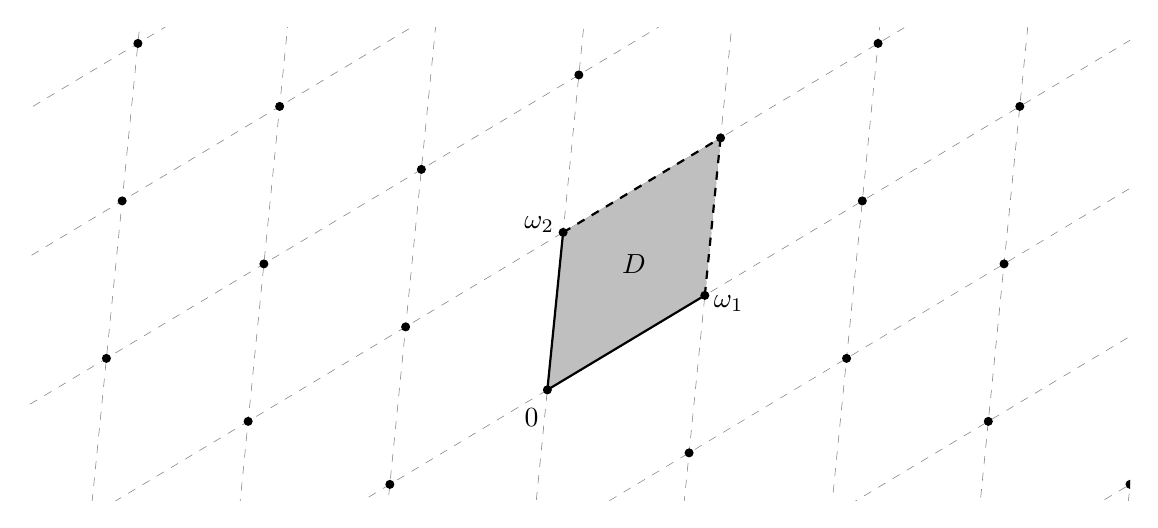
\begin{tikzpicture}
        \begin{scope}
            \clip (0,0) rectangle (14cm,6cm); % Clips the picture...
            \pgftransformcm{1}{0.6}{0.1}{1}{\pgfpoint{3cm}{3cm}} % This is actually the transformation
            %  matrix entries that gives the slanted
            % unit vectors. You might check it on
            % MATLAB etc. . I got it by guessing.
            
            \draw (4,-1.9) node [left]{$\omega_2$};
            \draw (3.8,-4) node [below]{$0$};
            \draw (6,-4.1) node [right]{$\omega_1$};
            \draw[style=help lines,dashed] (-14,-14) grid[step=2cm] (18,14); % Draws a grid in the new coordinates.
            \fill[fill=gray!50] (4,-4) rectangle (6,-2); % Puts the shaded rectangle
            % \fill[fill = gray!50] (0,0.5) rectangle (5,5);
            \draw[black, thick] (4,-4) -- (6,-4);
            \draw[black, thick] (4,-4) -- (4,-2);
            \draw[black, thick, dashed] (4,-2) -- (6,-2);
            \draw[black, thick, dashed] (6,-4) -- (6,-2);

            \draw (5,-3) node {$D$};
            \foreach \x in {-7,-6,...,8}{                           % Two indices running over each
            \foreach \y in {-7,-6,...,8}{                       % node on the grid we have drawn 
            \node[draw,circle,inner sep=1pt,fill] at (2*\x,2*\y) {}; % Places a dot at those points
            }
            }
        \end{scope}
    \end{tikzpicture}

    \caption{Mreža $\Lambda$ in fundamentalni paralelogram $D$.}
    \label{mreza}
\end{figure}

Na kompleksno ravnino $\C$ vpeljimo relacijo 
\[
    z \sim w \iff z - w \in \Lambda \quad \text{ za vsaka $z,w \in \C$.}
\]
To pomeni, da identificiramo vsaki dve točki, ki se razlikujeta kvečjemu za prišteto periodo $\omega \in \Lambda$. 
Brez težav se lahko prepričamo, da je to ekvivalenčna relacija na $\C$. Tako lahko tvorimo kvocientno množico $\C/_{\sim}$, katere ekvivalenčne razrede bomo označevali z $z + \Lambda$ in jih imenovali \emph{translati}, saj si jih lahko predstavljamo kot za vektor $z$ translirano mrežo $\Lambda$. Pripadajoča kvocientna projekcija bo $\pi : \C \to \C/_{\sim}$. Kvocient $\C/_{\sim}$ bomo od tod dalje rajši označevali s $\C/\Lambda$. 

Zaenkrat bomo $\C/\Lambda$ razumeli zgolj kot kvocientno množico, kasneje pa ga bomo opremili s topologijo, ki nam bo razkrila, da je ta prostor v resnici homeomorfen torusu. Za tem bomo definirali še kompleksno strukturo, ki nam bo na njem omogočila definirati holomorfne preslikave.


\begin{definicija}
    \emph{Fundamentalni paralelogram} za mrežo $\Lambda = \langle \om_1, \om_2 \rangle$ je
    \[
        D_{\alpha} = \{\alpha + t_1 \om_1 + t_2 \om_2 \mid t_1, t_2 \in [0,1)\}.
    \]
    Zaprtje fundamentalnega paralelograma $D_\alpha$ v $\C$ bomo označili z $\ols{D}_\alpha$. 
\end{definicija}

\begin{opomba}
    Kadar bomo govorili o fundamentalnih paralelogramih pogosto izbira izhodišča $\alpha$ ne bo pomembna, zato ga bomo tedaj izpustili in pisali samo $D$. V tem primeru lahko privzamemo, da je s tem mišljen $D_0$. 
\end{opomba}

Naslednja lema pove, da je preslikava $D_\alpha \to \C/\Lambda$ bijekcija med možicama. 

\begin{lema}
    \label{enolicni predstavnik}
    Poljuben translat $z + \Lambda$ mreže $\Lambda \subseteq \C$ ima natanko enega predstavnika v fundamentalnem paralelogramu $D_\alpha$. 
\end{lema}

\begin{dokaz}
    Ker sta osnovni periodi $\omega_1, \omega_2$ $\R$-linearno neodvisni, tvorita bazo za $\C$ gledano kot realen vektorski prostor. Tako lahko zapišemo $z - \alpha = a_1 \om_1 + a_2 \om_2$, kjer sta $a_1, a_2 \in \R$. Tedaj za 
    \[
        t_i = a_i - \lfloor a_i \rfloor \in [0,1) \quad \text{ za $i \in \{1,2\}$},
    \] 
    kjer $\lfloor x \rfloor$ označuje največje celo število, ki ni večje od $x$, velja $\alpha + t_1\om_1 + t_2 \om_2 = z - \lfloor a_1 \rfloor \om_1 - \lfloor a_2 \rfloor \om_2 \in D_\alpha \cap (z + \Lambda)$.
\end{dokaz}

Spomnimo se, da so \emph{holomorfne} funkcije na neki odprti domeni $D$ tiste, ki jih je mogoče odvajati v kompleksnem smislu povsod na $D$. Kolobar holomorfnih funkcij na $D$ označimo z $\hol{D}$. Če je funkcija holomorfna na celotnem $\C$, pravimo, da je \emph{cela holomorfna} funkcija. Množico teh označimo z $\hol{\C}$.

Če je $S \subseteq D$ diskretna množica brez stekališč v $D$, potem funkcijam, ki so holomorfne na $D \setminus S$, v točkah iz $S$ pa imajo pole, pravimo \emph{meromorfne} funkcije, točkam iz $S$ pa \emph{singularnosti}. Vsako meromorfno funkcijo $f$ na $D \subseteq \C$, lahko vidimo tudi kot preslikavo $D \to \RS$, kjer dodatno definiramo 
\[
    f(w) = \infty \quad \text{za vsak $w \in S$.} 
\]

\begin{definicija}
    Naj bo $f$ meromorfna funkcija na $\C$ in $\Lambda \subseteq \C$ mreža. Če za $f$ velja
    \[
        f(z + \om) = f(z) \quad \text{za vse $\om \in \Lambda$ in $z \in \C$},
    \]
    potem pravimo, da je $f$ \emph{eliptična} oziroma \emph{dvojno periodična} funkcija. Kadar želimo poudariti, da je $f$ eliptična glede na mrežo $\Lambda$, pravimo, da je \emph{$\Lambda$-periodična}. Polje $\Lambda$-periodičnih funkcij označimo s $\C(\Lambda)$. % mogoče tega zadnjega ne rabim
\end{definicija}




%%%%% Lastnosti eliptičnih funkcij %%%%%

\subsection{Lastnosti eliptičnih funkcij}

Sedaj si bomo pogledali nekaj izrekov, ki opisujejo naravo eliptičnih funkcij in jih lahko povečini pripišemo Liouvillu. Prvi je direktna posledica njegovega slavnega izreka iz kompleksne analize, ki pove, da razen konstant celih omejenih holomorfnih funkcij ni. Dokaz tega izreka lahko najdemo v \cite[izrek 59]{Globevnik}.

\begin{izrek}
    \label{cele el. funkcije}
    Naj bo $f$ cela eliptična funkcija. Tedaj je $f$ konstantna.
\end{izrek}

\begin{dokaz}
    Ker je $f$ konstantna na ekvivalenčnih razredih množice $\C/\Lambda$, \tj translatih oblike $z + \Lambda$, je enolično določena že z vrednostjo na enem od predstavnikov vsakega translata. Po lemi \ref{enolicni predstavnik} vidimo, da lahko predstavnika poljubnega translata najdemo v fundametnalnem paralelogramu $D$, zato bo 
    \[
        \sup_{z \in \C} \left\lvert f(z) \right\rvert = \sup_{z \in \olsi{D}} \left\lvert f(z) \right\rvert.
    \]
    % $f$ tako enolično določena že z vrednostmi na $D$. 
    Ker je $f$ holomorfna na celotnem $\C$, je tam seveda zvezna in je zato zvezna tudi na zaprtju fundamentalnega paralelograma $\olsi{D}$. To je zaprta in omejena množica v $\C$ in je tako kompaktna \cite[trditev 2.22]{MrcunTop}. Zvezna funkcija $f$ je na kompaktu $\olsi{D}$ omejena, kot eliptična funkcija pa je tako omejena na celotnem $\C$ \cite[posledica 2.28]{MrcunTop}. Funkcija $f$ je torej omejena in cela holomorfna, zato je po Liouvillovem izreku konstantna.  
\end{dokaz}

\begin{opomba}
    Enako lahko sklepamo tudi, če $f$ nima ničel. Tedaj je $1/f$ cela eliptična funkcija, ko jo v polih $f$ razširimo z $0$.
\end{opomba}

\begin{lema}
    \label{odvod el. funkcije}
    Naj bo $f \in \elf$ eliptična funkcija. Tedaj je tudi njen odvod $f' \in \elf$ eliptična funkcija.
\end{lema}

\begin{dokaz}
    Recimo, da je $z \in \C$ točka, kjer $f$ nima pola, zato je v njeni okolici holomorfna in jo lahko odvajamo v kompleksnem smislu. Z odvajanjem osnovnega pogoja za eliptične funkcije dobimo
    \[
        f'(z + \omega) = f'(z) \quad \text{ za vsak $\omega \in \Lambda$.}
    \]
    Če je v točki $z \in \C$ pol, pa ima tudi $f'$ v tej točki pol, torej pogoj za eliptičnost velja povsod na $\C$ in tako je $f' \in \elf$.
\end{dokaz}

% mogoče bi splošne domene ki jih označujem z D zamenjal z \Omega, in imel D rezerviran izključno za fundamentalni paralelogram. 
Vpeljimo nekaj notacije, ki jo bomo potrebovali v naslednjih izrekih. Če je $f$ meromorfna funkcija na odprti domeni $D \subseteq \C$, pravimo, da ima $f$ \emph{red $m \in \Z$} v točki $z_0 \in D$, če obstaja okolica $U \subseteq D$ točke $z_0$ in holomorfna funkcija $g \in \hol{U}$, ki je neničelna povsod na $U$, da velja 
\[
    f(z) = (z - z_0)^m g(z) \quad \text{za vse $z \in U$.}  
\]   
Tedaj označimo $\ord{z_0}{f} = m$. Če je $m > 0$, ima $f$ v $z_0$ \emph{ničlo} reda $m$, če pa je $m < 0$, ima $f$ v $z_0$ \emph{pol} reda $-m$.

\emph{Residuum} ali \emph{ostanek} funkcije $f$ pri točki $z_0 \in D$, je koeficient pred potenco $(z-z_0)\inv$ v Laurentovi vrsti za $f$ okrog $z_0$. Označimo ga z $\res{z_0}{f}$. 

% \begin{komentar}
%     Z $\sum_{w \in \torus}$ bomo označili vsoto po $w \in D$ poljubnem fundamentalnem paralelogramu, ki pripada merži $\Lambda$ in katerega rob ne vsebuje ničel ali polov funkcije $f$.   
% \end{komentar}

\begin{izrek}
    \label{liouville}
    Naj bo $f \in \C(\Lambda)$ eliptična funkcija in $D$ fundamentalni paralelogram glede na mrežo $\Lambda$, katerega rob $\partial D$ ne vsebuje polov ali ničel $f$. Tedaj velja
    \begin{flalign*}
        &\sum_{w \in D} \res{w}{f} = 0 && \label{eq: identiteta 1} \tag{i} \\ 
        &\sum_{w \in D} \ord{w}{f} = 0 && \label{eq: identiteta 2} \tag{ii} \\
        &\sum_{w \in D} \ord{w}{f}\cdot w \in \Lambda. && \label{eq: identiteta 3} \tag{iii}
    \end{flalign*}

    % \begin{enumerate}[(a)]
    %     \item \[\sum_{w \in D} \res{w}{f} = 0\] \label{identiteta 1}
    %     \item \[\sum_{w \in D} \ord{w}{f} = 0\] \label{identiteta 2}
    %     \item \[\sum_{w \in D} \ord{w}{f}\cdot w \in \Lambda.\] \label{identiteta 3}
    % \end{enumerate}    
\end{izrek}

\begin{dokaz}
    \par
    \eqref{eq: identiteta 1} Uporabimo izrek o ostankih \cite[izrek 71]{Globevnik}, ki pove
    \[
        \sum_{w \in D} \res{w}{f} = \frac{1}{2\pi i}\int_{\partial D} f(z)dz.  
    \]
    Razdelimo rob fundametalnega paralelograma $\partial D = \sigma_1 \cup \sigma_2 \cup \sigma_3 \cup \sigma_4$ na štiri daljice, ki ga omejujejo, kot prikazuje slika \ref{fundamentalni paralelogram}.

    \begin{figure}[H]
        \centering
        
\begin{tikzpicture}
            \begin{scope}
                \clip (0,0) rectangle (14cm,4cm); % Clips the picture...
                \pgftransformcm{1}{0.6}{0.1}{1}{\pgfpoint{2cm}{2cm}};
                \fill[fill=gray!50] (4,-4) rectangle (6,-2);
                % \fill[fill = gray!50] (0,0.5) rectangle (5,5);
                \draw (4,-1.9) node [left]{$\alpha + \omega_2$};
                \draw (3.9,-4) node [below]{$\alpha$};
                \draw (6,-4.1) node [right]{$\alpha + \omega_1$};
                \draw (5,-3) node {$D$};
                \draw (3.95,-3) node [left]{$\sigma_4$};
                \draw (5.2,-4.2) node [below]{$\sigma_1$};
                \draw (6.1,-3.1) node [right]{$\sigma_2$};
                \draw (4.8,-1.8) node [above]{$\sigma_3$};

                % \draw[postaction={decorate}] (4,-4)--(4,-2);
                
                \foreach \x in {4,6}{                          
                    \foreach \y in {-4,-2}{                       
                        \node[draw,circle,inner sep=1pt,fill] at (\x,\y) {}; 
                    }
                };

                \begin{scope}[thick,decoration={
                    markings,
                    mark=at position 0.5 with {\arrow{stealth}}
                        }
                    ] 
                    \draw[postaction={decorate}] (4,-4)--(6,-4);
                    \draw[postaction={decorate}] (6,-4)--(6,-2);
                    \draw[postaction={decorate}] (6,-2)--(4,-2);
                    \draw[postaction={decorate}] (4,-2)--(4,-4);
                \end{scope}
            \end{scope}

        \end{tikzpicture}
        
        \caption{Fundamentalni paralelogram.}
        \label{fundamentalni paralelogram}
    \end{figure}


    Jasno tedaj velja
    \[
        \int_{\partial D} f(z)dz = \int_{\sigma_1} f(z)dz + \int_{\sigma_2} f(z)dz + \int_{\sigma_3} f(z)dz + \int_{\sigma_4} f(z)dz.
    \]
    % Z zamenjavo spremenljivk $w = z + \om_1$ v prvem in $w = z + \om_2$ v četrtem interalu je zaradi periodičnosti $f$ preprosto videti, da se integrala po parih nasprotnih stranic ($\sigma_1$ in $\sigma_3$ ter $\sigma_2$ in $\sigma_4$) odštejeta, kar nam da želeni rezultat. 
    Z menjavo spremenljivk $w = z + \om_2$ v prvem in $w = z + \om_1$ v četrtem integralu je zaradi periodičnosti $f$ in orientacije obeh parov nasprotnih stranic ($\sigma_1$ in $\sigma_3$ ter $\sigma_2$ in $\sigma_4$) razvidno, da se integrala po parih nasproti ležečih stranic izničita, kar nam da želeni rezultat $0$.
    
    \eqref{eq: identiteta 2} Po lemi \ref{odvod el. funkcije} je $f' \in \elf$, zato je tudi kvocient $f'/f$ eliptičen. Tedaj velja
    \[
        \sum_{w \in D} \ord{w}{f} = \frac{1}{2\pi i}\int_{\partial D} \frac{f'(z)}{f(z)}dz = 0, 
    \]
    kjer smo v prvi enakosti uporabili princip argumenta \cite[Izrek 72]{Globevnik}, druga enakost pa je identiteta \eqref{eq: identiteta 1}, ki velja zaradi eliptičnosti kvocienta $f'/f$.

    % mogoče bom povsod zamenjal $z_0$ z $w$...
    \eqref{eq: identiteta 3} Oglejmo si funkcijo $z \mapsto z \frac{f'(z)}{f(z)}$. Jasno je ta funkcija meromorfna na $\C$. Naj bo $z_0 \in \C$ poljuben. Tedaj obstaja $m \in \Z$, okolica $U \subseteq \C$ točke $z_0$ in holomorfna funkcija $g \in \hol{U}$, ki je neničelna na $U$, da velja
    \[
        f(z) = (z - z_0)^m g(z) \quad \text{ za vsak $z \in U$.}  
    \]
    Z odvajanjem te enakosti dobimo
    \[
        f'(z) = m(z - z_0)^{m - 1} g(z) + (z - z_0)^m g'(z),
    \]
    ki prav tako velja povsod na $U$. Skupaj tako dobimo, da za vsak $z \in U$ velja
    \[
        z\frac{f'(z)}{f(z)} = \frac{mz}{z-z_0} + z\frac{g'(z)}{g(z)} = \frac{mz_0}{z-z_0} + \underbrace{m + z\frac{g'(z)}{g(z)}}_{\in \hol{U}}.
    \]
    Ker sta zadnja dva člena holomorfna na $U$, edino člen $\frac{mz_0}{z-z_0}$ prispeva h glavnemu delu Laurentovega razvoja funkcije $z \mapsto z \frac{f'(z)}{f(z)}$ okrog $z_0$. Zato je 
    \[
        \operatorname{res}_{z_0} \left( z \frac{f'(z)}{f(z)} \right) = mz_0 = \ord{z_0}{f}z_0.  
        % \res{z_0}{z \frac{f'(z)}{f(z)}} = mz_0 = \ord{z_0}{f}z_0.  
    \]
    Tako dobimo 
    \[
        \sum_{w \in D} \ord{w}{f}\cdot w 
        = \sum_{w \in D} \operatorname{res}_{w} \left( z \frac{f'(z)}{f(z)} \right)
        = \frac{1}{2 \pi i} \int_{\partial D} z \frac{f'(z)}{f(z)}dz. 
    \] 
    Poglejmo si sedaj zadnji integral, ki ga podobno kot pri dokazu formule \eqref{eq: identiteta 1} razbijemo na vsoto integralov po štirih stranicah. Argument o odštevanju integralov po nasprotnih stranicah paralelograma pa tokrat zaradi neperiodičnosti funkcije $z \mapsto z \frac{f'(z)}{f(z)}$ v splošnem ne bo deloval. Z uvedbo nove spremenljivke $w = z + \omega_2$ v integral po stranici $\sigma_1$ vidimo
    \begin{multline*}
        \int_{\sigma_1} z \frac{f'(z)}{f(z)}dz = 
        \int_{\sigma_1} z \frac{f'(z + \omega_2)}{f(z + \omega_2)}dz = \\ = 
        - \int_{\sigma_3} (w - \omega_2) \frac{f'(w)}{f(w)}dw = 
        - \int_{\sigma_3} z \frac{f'(z)}{f(z)}dz + \omega_2 \int_{\sigma_3} \frac{f'(z)}{f(z)}dz.
    \end{multline*}
    Podobno z uvedbo nove spremenljivke $w = z + \omega_1$ storimo z integralom po stranici $\sigma_4$ in tako dobimo
    \[
        \int_{\partial D} z \frac{f'(z)}{f(z)}dz = \omega_1 \int_{\sigma_4} \frac{f'(z)}{f(z)}dz + \omega_2 \int_{\sigma_3} \frac{f'(z)}{f(z)}dz.
    \]

    Za poljubno sklenjeno in odsekoma gladko krivuljo $\gamma : [0,1] \to \C$, tj. $\gamma(0) = \gamma(1)$, ki ne poteka skozi izhodišče $0\in \C$, je
    \[
        \frac{1}{2 \pi i} \int_\gamma \frac{dz}{z} \in \Z
    \]
    \emph{ovojno število} krivulje $\gamma$ okoli $0$ in nam pove, kolikokrat se krivulja $\gamma$ ovije okoli izhodišča. Podrobnosti o tem lahko bralec najde v \cite[4.2.1.]{Ahlfors}.

    Osredotočimo se sedaj samo na prvi integral, premislek za drugega je analogen. Opazimo, da je zaradi eliptičnosti $f$ krivulja $f(\sigma_4)$ sklenjena, saj sta krajišči daljice $\sigma_4$ točki $\alpha$ in $\alpha + \omega_2$, v katerih ima $f$ enaki vrednosti. Pot $\gamma : [0,1] \to f(\sigma_4)$, ki predstavlja to sklenjeno krivuljo, je podana s predpisom $t \mapsto f(\alpha + t\omega_2)$. Opomnimo še, da to ni nujno parametrizacija krivulje v običajnem smislu, saj je lahko neinjektivna. 
    
    Zapišemo lahko 
    \[
        2 \pi i k_1 = 
        \int_{\gamma} \frac{dz}{z} = 
        \int_0^1 \frac{\gamma'(t)}{\gamma(t)}dt =
        \int_0^1 \frac{f'(\alpha + t\omega_2)}{f(\alpha + t\omega_2)}\omega_2 dt = 
        \int_{\sigma_4} \frac{f'(z)}{f(z)}dz
    \]
    za neki $k_1 \in \Z$. Podobno je tako tudi
    \[
        2 \pi i k_2 = \int_{\sigma_3} \frac{f'(z)}{f(z)}dz,
    \]
    za neki $k_2 \in \Z$. Skupaj je torej 
    \[
        \sum_{w \in D} \ord{w}{f} \cdot w = 
        \frac{1}{2 \pi i} \int_{\partial D} z\frac{f'(z)}{f(z)}dz = 
        k_1 \omega_1 + k_2 \omega_2\in \Lambda.  
    \]
\end{dokaz}

\begin{opomba}
    \label{liouville opomba}

    (1) V vseh treh točkah seštevamo po neštevnem fundamentalnem paralelogramu $D$, toda vse tri vsote vsebujejo zgolj končno mnogo neničelnih členov. Residuum in red funkcije $f$, sta lahko različna od nič samo v ničlah ali polih $f$, teh pa je v kompaktu $\olsi{D}$ lahko le končno, saj bi sicer prišli v nasprotje s principom identičnosti. Ta pravi, da se meromorfni funkciji, definirani na neki odprti domeni $\Omega$, ki se ujemata na množici s stekališčem v $\Omega$, ujemata povsod na $\Omega$.
    %  \cite[]{}.
     
    (2) Kot nakazuje izrek, je izbira fundamentalnega paralelograma irelevantna, dokler ta izpolnjuje določene predpostavke o robu. Kljub temu pa se prepričajmo, da lahko vselej takšen fundamentalni paralelogram vedno izberemo. 

    Denimo, da to ni mogoče, torej da ima vsak fundamentalni paralelogram na svojem robu vsaj en pol eliptične funkcije $f$. S translacijami
    \[
        \tau_n : z \mapsto z + \frac{1}{n}(\om_1 + \om_2); \quad n\in \N
    \]
    delujemo na rob fundamentalnega paralelograma $\partial D$ in tako dobimo števno mnogo različnih polov za $f$. To zaporedje polov leži v uniji $\bigcup_{n \in \N} \tau_n(\partial D)$, ki jo lahko zapremo v dovolj velik zaprt disk. Na ta način dobimo zaporedje polov v kompaktu, ki ima po Bolzano-Weierstrassovem izreku stekališče, kar pa je v nasprotju s tem, da je množica polov meromorfne funkcije diskretna v $\C$. 
    
    Podobno lahko hkrati sklepamo še za ničle funkcije $f$ in s pomočjo principa identičnosti pridemo v nasprotje z diskretnostjo množice ničel meromorfne funkcije $f$.
    
    (3) Formula \eqref{eq: identiteta 2} pove, da ima eliptična funkcija na fundamentalnem paralelogramu enako število ničel in polov štetih z večkratnostjo. 

\end{opomba}

\begin{definicija}
    \emph{Red} eliptične funkcije je število polov šteto z večkratnostjo v poljubnem fundamentalnem paralelogramu. 
\end{definicija}

Tudi, če pol $z_0$ leži na robu $\partial D$ izbranega fundamentalnega paralelograma, lahko govorimo o redu tega pola v $D$. Takrat štejemo \emph{red pola $z_0$ v $D$} kot $\frac{1}{2}\ord{z_0}{f}$, če pol ni eno od štirih oglišč, oziroma, v primeru, ko je pol $z_0$ oglišče paralelograma, vzamemo za njegov red vrednost
\[
    \frac{\ell(\partial \Delta(z_0, r) \cap D)}{2 \pi r}\ord{z_0}{f}.
\]
Ob tem $\ell$ opisuje dolžino danega krožnega loka, $r > 0$ pa je dovolj majhen, da je $z_0$ edino oglišče fundamentalnega paralelograma, vsebovano v odprtem disku ${\Delta(z_0, r) =}$ ${\{z \in \C \mid \left\lvert z - z_0 \right\rvert < r\}}$. Z drugimi besedami je ta količina normaliziran notranji kot fundamentalnega paralelograma pri oglišču $z_0$ pomnožen, z $\ord{z_0}{f}$.  

\begin{zgled*}
    Naj bo $\rho = e^{2\pi i /3}$ in $\Lambda = \Z + \rho\Z$. Fundamentalni paralelogram $D$ te mreže je torej romb v kompleksni ravnini z oglišči $0$, $1$, $\rho$ in $1 + \rho$. Naj bo $f$ eliptična funkcija s poli v mreži $\Lambda$. Tedaj bo red pola $0$ za $f$ v $D$ enak
    \[
        \frac{2\pi/3}{2\pi}\ord{0}{f} = \frac{1}{3}\ord{0}{f},
    \]
    saj je notranji kot romba $D$ v oglišču $0$ enak $2\pi/3$, red pola $\rho$ za $f$ v $D$ pa bo enak
    \[
        \frac{\pi/3}{2\pi}\ord{\rho}{f} = \frac{1}{6}\ord{\rho}{f},
    \]
    saj stranici, ki se srečata v $\rho$, skupaj oklepata kot velikosti $\pi/3$.
\end{zgled*}

\begin{posledica}
    \label{poseldica o redu elipticne funkcije}
    Nekonstantna eliptična funkcija ima red vsaj $2$.
\end{posledica}

\begin{dokaz}
    Brez škode za splošnost denimo, da je $f \in \elf$ nekonstantna eliptična funkcija z enim (enostavnim) polom $\alpha$ na fundamentalni domeni $D$, saj po izreku \ref{cele el. funkcije} že vemo, da bi bila $f$ konstantna, če bi bila brez polov. 
    % da bi bila konstantna, če ne bi imela nobenega pola po izreku \ref{cele el. funkcije}.
    Predpostavimo lahko tudi, da pol leži v notranjosti $D$. Z integracijo po robu $\partial D$ tako dobimo neničelni residuum
    \[
        \frac{1}{2 \pi i} \int_{\partial D} f(z)dz = \res{\alpha}{f} \neq 0.  
    \]
    To pa je v nasprotju s formulo \eqref{eq: identiteta 1} iz izreka \ref{liouville}, ki pove, da je ta residuum -- kot edini člen v vsoti -- enak nič. 
\end{dokaz}

\begin{posledica}
    \label{elipticna funkcija je surjektivna}
    Nekonstantna eliptična funkcija $f: \C \to \RS = \C \cup \{\infty\}$ je surjektivna. 
\end{posledica}

\begin{dokaz}
    Ker je $f \in \elf$ nekonstantna, ima po izreku \ref{cele el. funkcije} pol in lahko zato rečemo, da tam doseže točko $\infty$. Naj bo sedaj $w \in \C$ poljubna točka in pokažimo, da obstaja $z \in \C$, da velja $f(z) = w$.
    
    Definirajmo $g(z) := f(z) - w$. Funkcija $g$ je prav tako eliptična in ima pol, saj je takšna $f$ in prištevanje konstante na ti dve lastnosti nima vpliva. Po opombi \ref{liouville opomba} (3) ima $g$ ničlo v $\C$, kar pokaže želeno.
\end{dokaz}



%%%%% Weierstrassova funkcija %%%%%

\subsection{Weierstrassova funkcija $\wp$}

Osrednja tema tega poglavja, ki bo povezala eliptične krivulje s kompleksnimi torusi in za katero je bilo potrebno razvijati teorijo v prejšnjem razdelku, bo najprej definicija nato pa pregled lastnosti \ti \emph{Weierstrassove funkcije} $\wp$. 

Vseskozi naj bo $\Lambda$ mreža v $\C$ in naj velja oznaka $\Lambda' = \Lambda \setminus \{0\}$.

\begin{definicija}
    \label{eisensteinova vrsta}
    Za celo število $k > 2$ je \emph{Eisensteinova vrsta reda $k$} podana kot
    \[
        G_k(\Lambda) = \sum_{\om \in \Lambda'} \frac{1}{\om^k}.  
    \]
\end{definicija}

\begin{opomba}
    Opazimo, da za lihe $k$ velja $G_k(\Lambda) = 0$, saj se člena pri $\om$ in $-\om$ v vsoti odštejeta. 
\end{opomba}

\begin{lema}
    \label{lema o konvergenci eisensteinove vrste}
    Za vsako celo število $k > 2$ je Eisensteinova vrsta reda $k$ absolutno konvergentna.
\end{lema}

\begin{dokaz}
    Za vsak $n \in \N$ definirajmo množice
    \[
        C_n = \{k_1 \om_1 + k_2 \om_2\in \Lambda \mid \abs{k_1} + \abs{k_2} = n\}.  
    \]
    Induktivni sklep pokaže, da je moč posamezne od teh množic $C_n$ enaka $4n$.
    % Preprosto se je prepričati, da je moč posamezne od teh množic $\#C_n = 4n$. 
    Vsak element $\om \in C_n$ pa lahko po absolutni vrednosti ocenimo $\left\lvert \om \right\rvert \geq \rho n$, kjer je $\rho > 0$ razdalija od izhodišča $0$, do roba paralelograma z oglišči v točkah $\pm \om_1, \pm \om_2$. Tedaj velja ocena
    \[
        \sum_{\om \in \Lambda'} \frac{1}{\left\lvert  \om^k \right\rvert} = 
        \sum_{n = 1}^\infty \sum_{\om \in C_n} \frac{1}{\left\lvert  \om \right\rvert^k} \leq
        \sum_{n = 1}^\infty \sum_{\om \in C_n} \frac{1}{(\rho n)^k} =
        \sum_{n = 1}^\infty \frac{4n}{\rho^k n^k} = 
        \frac{4}{\rho^k} \sum_{n = 1}^\infty \frac{1}{n^{k-1}}.
    \]
    Klasičen rezultat iz realne analize pove, da zadnja vrsta konvergira natanko tedaj, ko je $k - 1 > 1$ in tako po primerjalnem kriteriju dobimo absolutno kovergenco Eisensteinove vrste $\sum_{\om \in \Lambda'} \om^{-k}$.
\end{dokaz}

\begin{lema}
    \label{lema o absolutni in enakomerni konvergenci}
    Za vsako celo število $k > 2$ vrsta 
    \[
        \sum_{\om \in \Lambda'} \frac{1}{(z - \om)^k}
    \]
    konvergira absolutno za poljuben $z\in \C\setminus\Lambda'$ in enakomerno po kompaktih na $\C \setminus \Lambda'$. 
\end{lema}

\begin{dokaz}
    Glavna ideja dokaza bo s pomočjo nekaj ocen uporabiti Weierstrassov M-test. Naj bo $K \subseteq \C$ poljuben kompakt disjunkten z $\Lambda'$. Kot tak je omejen, zato je vsebovan v nekem disku $\Delta(0,r)$ z radijem $r > 0$. Razdelimo obravnavo period $\omega \in \Lambda'$ na tiste, ki ležijo v disku $\Delta(0,2r)$, in na tiste, ki ne.
    \begin{enumerate}[(i)]
        \item 
    Zaradi kompaktnosti množice $K$ za vse $\omega \in \Lambda' \cap \Delta(0,2r)$ obstaja minimum
    \[
        \min_{z \in K} \abs{z - \omega} =: \epsilon_\omega > 0.
    \]
    Ker pa je takšnih period, za katere je $\abs{\omega} < 2r$, zgolj končno mnogo, denimo $n \in \N$, lahko za $\epsilon$ izberemo najmanjšega izmed $\epsilon_\om$ in tako velja 
    \[
        \abs{z - \omega} \geq \epsilon \quad \text{za vse $z \in K$ in vse $0 < \abs{\omega} < 2r$.}  
    \]
    
    \item
    Za vse periode $\abs{\omega} \geq 2r$ preko trikotniške neenakosti
    \[
        \abs{\om} \leq \abs{z - \om} + \abs{z} \quad \text{za vse $z \in K$}
    \]
    vidimo, da velja 
    \[
        \abs{z - \om} \geq 
        \abs{\om} - \abs{z} \geq 
        \abs{\om} - r \geq 
        \abs{\om} - \frac{1}{2}\abs{\om} \geq
        \frac{1}{2}\abs{\om} \quad \text{za vse $z\in K$.}
    \]
    \end{enumerate}
    Tako pridemo do ocene
    \[
        \sum_{\om \in \Lambda'} \frac{1}{\abs{z - \om}^k} = 
        \sum_{\substack{\om \in \Lambda' \\ \abs{\om} < 2r}} \frac{1}{\abs{z - \om}^k} + \sum_{\substack{\om \in \Lambda' \\ \abs{\om} \geq 2r}} \frac{1}{\abs{z - \om}^k} \leq
        \frac{n}{\epsilon^k} + \sum_{\substack{\om \in \Lambda' \\ \abs{\om} \geq 2r}} \frac{2^k}{\abs{\om}^k},
    \]
    ki velja povsod na $K$. Ker je zadnja vsota del (po lemi \ref{lema o konvergenci eisensteinove vrste}) absolutno konvergentne Eisensteinove vrste reda $k$, nam Weierstrassov M-test zagotovi želeni rezultat.
\end{dokaz}

V nadaljevanju bomo obravnavali različne funkcijske vrste holomorfnih (meromorfnih) funkcij, za katere bi se radi preričali, da se tudi seštejejo v holomorfne funkcije. Naslednji izrek, ki ga samo nevedemo, nam pove, da je zadosten pogoj za to zahtevo v bistvu samo njihova enakomerna konvergenca po komapktih. 

\begin{izrek}[\protect{\cite[izrek 64]{Globevnik}}]
    % \cite[\S 5, Theorem 1]{Ahlfors}
    \label{izrek o konvergenci holomorfnih funkcij}
    Naj bo $(f_n)_{n \in \N}$ zaporedje holomorfnih funkcij na odprti domeni $\Omega \subseteq \C$, ki enakomerno po kompaktih v $\Omega$ konvergira k limitni funkciji $f$. Tedaj je tudi $f$ holomorfna na $\Omega$ in zaporedje odvodov $(f'_n)_{n\in \N}$ konvergira enakomerno po kompaktih v $\Omega$ k odvodu limitne funkcije $f'$.
\end{izrek}
    
Oglejmo si sedaj funkcijo $f:\C\setminus\Lambda \to \C$, podano s predpisom
\[
    f(z) = \sum_{\om \in \Lambda} \frac{1}{(z - \om)^k}, \quad k > 2.
\]
Zaradi absolutne konvergence te vrste jo lahko seštevamo v poljubenem vrstnem redu. Če to storimo postopoma po diskih $\disk{0}{n}$ za $n\in\N$, dobimo zaporedje delnih vsot, ki so holomorfne na $\C\setminus\Lambda$ in konvergirajo k $f$. Poleg tega zaradi leme \ref{lema o absolutni in enakomerni konvergenci} že vemo, da ta vrsta konvergira tudi enakomerno po kompaktih v $\C\setminus\Lambda$, torej na tej domeni $f$ določa holomorfno funkcijo po izreku \ref{izrek o konvergenci holomorfnih funkcij}. Dodatno ima $f$ v vsakem $\om_0 \in \Lambda$ pol reda $k$ in residuum $0$, o čemer se lahko prepričamo, ko na neki dovolj majhni prebodeni okolici točke $\om_0$ zapišemo
% po lemi \ref{lema o absolutni in enakomerni konvergenci} lahko predstavimo, da jo seštevamo postopoma po diskih $\disk{0}{n}$ za $n\in\N$ in tako dobimo zaporedje delnih vsot, ki so holomorfne na $\C\setminus\Lambda$ in konvergirajo k $f$. Po izreku \ref{izrek o konvergenci holomorfnih funkcij} je $f$ holomorfna na $\C \setminus \Lambda$, v vsakem $\om_0 \in \Lambda$ pa ima pol reda $k$ in residuujem $0$. O tem se prepričamo, saj lahko zapišemo
\[
    f(z) = \frac{1}{(z-\om_0)^k} + \sum_{\om \in \Lambda \setminus \{\om_0\}} \frac{1}{(z - \om)^k}.
\]
% na neki dovolj majhni prebodeni okolici točke $\om_0$. 
H glavnemu delu okrog $\om_0$ prispeva samo člen $(z - \om_0)^{-k}$, vrsta, ki ostane, pa je zaradi leme \ref{lema o absolutni in enakomerni konvergenci} po podobnem razmisleku kot zgoraj holomorfna na tej prebodeni okolici in zato na glavni del nima vpliva. Tako je $f$ meromorfna funkcija na $\C$. 

\begin{primer*}
    \label{primer odvod wp}
    Zgornje nam omogoča konstruirati prvi netrivialen primer eliptične funkcije, ki bo koristen tudi v nadaljevanju. Prepričajmo se, da je funkcija, podana s predpisom
    \[
        f(z) = \sum_{\om \in \Lambda} \frac{1}{(z - \om)^3},
    \]
    ne le meromorfna, ampak res tudi eliptična. Če je $z \in \C$ poljuben in $\om_0 \in \Lambda$ poljubna perioda, vidimo, da velja
    \[
        f(z + \om_0) = 
        \sum_{\om \in \Lambda} \frac{1}{(z + \om_0 - \om)^3} = 
        \sum_{\om \in \Lambda} \frac{1}{(z - (\om - \om_0))^3} = 
        \sum_{\om \in \Lambda} \frac{1}{(z - \om)^3} = 
        f(z),
    \]
    kjer smo v predzadnji enakosti upoštevali, da je translacija $\om \mapsto \om - \om_0$ zgolj permutacija mreže $\Lambda$, ki samo premeša vrstni red seštevanja v zadnji (absolutno konvergentni) vrsti. 
\end{primer*}

Funkcija iz primera \ref{primer odvod wp} ima v vsaki periodi $\om\in \Lambda$ pol stopnje $3$ oziroma na fundamentalnem paralelogramu ima natanko pol stopnje $3$, torej bi lahko rekli, da je eliptična funkcija reda $3$. Posledica \ref{poseldica o redu elipticne funkcije} nam zagotavlja, da je spodnja meja za red nekonstantne eliptične funkcije enaka $2$, zato se je naravno vprašati, ali je ta meja kdaj dosežena. Poskusili bi lahko z vrsto $\sum_{\om\in\Lambda}(z - \om)^{-2}$, toda ta žal ne konvergira absolutno. Vseeno pa jo lahko nekoliko popravimo, kar nas privede do naslednje definicije. 

\begin{definicija}
    \emph{Weierstrassova eliptična funkcija $\wp$} glede na mrežo $\Lambda$ je
    \[
        \wp(z) = \frac{1}{z^2} + \sum_{\om\in\Lambda'}\left(\frac{1}{(z-\om)^2} - \frac{1}{\om^2}\right).
    \]
    Kadar želimo poudariti, da je ta prirejena mreži $\Lambda$, pišemo tudi $\wp_{\Lambda}$.
\end{definicija}

\begin{trditev}
    \label{lastnosti wp}
    Za Weierstrassovo funkcijo $\wp$ glede na mrežo $\Lambda$ veljajo naslednje trditve.
    \begin{itemize}
        \item[(i)] Vrsta, ki predstavlja funkcijo $\wp$, konvergira absolutno in enakomerno po kompaktih v $\C\setminus\Lambda'$, zato je $\wp$ holomorfna funkcija na $\C \setminus \Lambda$.
        \item[(ii)] $\wp$ je soda.
        \item[(iii)] $\wp$ je $\Lambda$-periodična.
        \item[(iv)] točke iz mreže $\Lambda$ so natanko poli Weierstrassove funkcije $\wp$. Vsi so stopnje $2$, residuumi v njih pa so vedno enaki $0$. 
    \end{itemize}
\end{trditev}

\begin{dokaz}
    (i) Naj bo $K \subseteq \C\setminus\Lambda$ kompakt in $r > 0$, da disk $\disk{0}{r}$ omejuje kompakt $K$. Podobno kot v dokazu leme \ref{lema o absolutni in enakomerni konvergenci} bomo obravnavo razdelili na periode $\om\in \Lambda$, ki ležijo znotraj diska $\disk{0}{2r}$, in na tiste, ki ležijo v njegovem komplementu. Na kompaktu $K$ že vemo, da lahko omejimo izraz
    \[
        \frac{1}{\abs{z^2}} + \sum_{\substack{\om\in\Lambda' \\ \abs{\om} < 2r}} \left\lvert\frac{1}{(z - \om)^2} - \frac{1}{\om^2}\right\rvert < M \quad \text{za vsak $z \in K$,}
    \]
    kjer je $M \in \R$.
    %  = n \cdot \max\{\max_{z \in K} \abs{z^{-2}}, \max_{\om\in\Lambda', \abs{\om} < 2r, z \in K} \abs{(z-\om)^{-2} - \om^{-2}}\}$ in je $n\in\N$ število period $\om\in\Lambda$, ki ležijo znotraj diska $\disk{0}{2r}$.
    Za periode $\om\in\Lambda, \abs{\om} \geq 2r$ in $z \in K$, že poznamo oceno $\abs{z - \om} \geq \abs{\om} - \abs{z} \geq \frac{1}{2}\abs{\om}$, izpeljemo pa še
    % \[
    %     \abs{z - \om} \geq \abs{\om} - \abs{z} \geq \frac{1}{2}\abs{\om}  
    % \] 
    % nato pa še
    \[
        \abs{2\om - z} \leq \abs{2\om} + \abs{z} \leq 3 \abs{\om}.
    \]
    Tako velja
    \[
        \abs{\frac{1}{(z - \om)^2} - \frac{1}{\om^2}} = 
        \abs{\frac{\om^2 - (z - \om)^2}{\om^2(z - \om)^2}} =
        \abs{\frac{z(2\om - z)}{\om^2 (z - \om)^2}} \leq
        \frac{r \cdot 3\abs{\om}}{\abs{\om}^2(\frac{1}{2}\abs{\om})^2} = 
        \frac{12r}{\abs{\om}^3},
    \]
    kar pomeni, da lahko del vsote, ki teče po $\om\in\Lambda', \abs{\om} \geq 2r$, navzgor omejimo s konstanto $12r$ pomnoženim (po lemi \ref{lema o konvergenci eisensteinove vrste}) konvergentnim delom vrste $\sum_{\om\in\Lambda'}\abs{\om}^{-3}$.

    Zaporedje holomorfnih delnih vsot je tako po Weierstrassovem M-testu absolutno in po kompaktih enakomerno konvergentno na $\C\setminus\Lambda$. Po izreku \ref{izrek o konvergenci holomorfnih funkcij} je limitna funkcija zaporedja -- tj. Weierstrassova funkcija $\wp$ -- holomorfna na $\C\setminus\Lambda$, vrsto pa lahko odvajamo členoma, kar pomeni, da je odvod funkcije $\wp$ enak
    \[
        \wp'(z) = \sum_{\om \in \Lambda}\frac{-2}{(z-\om)^3}. 
    \]

    (ii) Z računom se prepričamo
    \begin{multline*}
        \wp(-z) =   
        \frac{1}{(-z)^2} + \sum_{\om\in\Lambda'}\left(\frac{1}{(-z-\om)^2} - \frac{1}{\om^2}\right) \\ = 
        \frac{1}{z^2} + \sum_{\om\in\Lambda'}\left(\frac{1}{(z+\om)^2} - \frac{1}{(-\om)^2}\right) =
        \frac{1}{z^2} + \sum_{\om\in\Lambda'}\left(\frac{1}{(z-\om)^2} - \frac{1}{\om^2}\right) =
        \wp(z),
    \end{multline*}
    kjer smo za predzadnji enačaj upoštevali, da transformacija $\omega \mapsto -\omega$ samo premeša vrstni red seštevanja v absolutno konvergentni vrsti.

    (iii) Naj bo $\om\in \Lambda$ poljuben. Kot smo se prepričali v primeru \ref{primer odvod wp}, je $\wp'$ eliptična funkcija, zato je $\wp'(z + \om) - \wp'(z) = 0$, kar pomeni, da se funkciji $\wp(z + \om)$ in $\wp(z)$ razlikujeta zgolj za prišteto konstanto. Če v obe vstavimo $z = -\frac{\omega}{2}$ in upoštevamo sodost funkcije $\wp$, vidimo, da je ta konstanta enaka $0$, kar pokaže želeno.

    (iv) Zaradi $\Lambda$-periodičnosti funkcije $\wp$ po točki (iii) je dovolj situacijo obravnavati samo okoli točke $0\in\Lambda$. Podobno kot smo sklepali o polih funkcije $\sum_{\om\in\Lambda'}(z-\om)^{-k}$, tudi tukaj vidimo, da na neki prebodeni okolici točke $0$ h glavnemu delu Laurentove vrste za $\wp$ okoli $0$ prispeva le člen $z^{-2}$, ki nam da pol reda $2$ z residuujem $0$, preostanek vrste pa po dokazu točke (i) na tej prebodeni okolici definira holomorfno funkcijo, ki na glavni del nima vpliva.  
\end{dokaz}

Naše zanimanje za Weierstrassovo eliptično funkcijo se skriva v dejstvu, da ta funkcija zadošča posebni diferencialni enačbi oblike $\wp'(z)^2 = f(\wp(z))$, kjer je $f \in \C[x]$ kubični polinom, ki je v tesni povezavi z Weierstrassovo enačbo eliptične krivulje. Da bo ta povezava jasneje razvidna, si poglejmo Laurentov razvoj $\wp$ okoli izhodišča $0$. 

\begin{lema}
    Naj bo $\wp$ Weierstrassova eliptična funkcija glede na mrežo $\Lambda$. Njen Laurentov razvoj okoli točke $0$ je
    \begin{equation}
        \label{eq: Laurentov razvoj wp}
        \wp(z) = \frac{1}{z^2} + \sum_{k = 1}^\infty(2k + 1)G_{2k + 2}(\Lambda)z^{2k},  
    \end{equation}
    kjer $G_{2k}(\Lambda)$ označuje Eisensteinovo vrsto reda $2k$.
\end{lema}

\begin{dokaz}
    Najprej z odvajanjem geometrijske vrste za $(1 - x)^{-1}$ pri $\abs{x} < 1$ ugotovimo, da je 
    \[
        \frac{1}{(1 - x)^2} = \sum_{n = 0}^\infty (n + 1) x^n \quad \text{za $\abs{x} < 1$}  
    \]
    in ta konvergenca je enakomerna in absolutna na kompaktih v disku $\disk{0}{1}$. To uporabimo v izrazu
    \[
        \frac{1}{(z - \om)^2} - \frac{1}{\om^2} = 
        \frac{1}{\om^2}\left(\frac{1}{(1 - \frac{z}{\om})^2} - 1\right) = 
        \frac{1}{\om^2} \sum_{n = 1}^\infty (n + 1)\frac{z^n}{\om^{n}} = 
        \sum_{n = 1}^\infty (n + 1)\frac{z^n}{\om^{n + 2}}, 
    \]
    ki velja za vse $\om\in\Lambda'$ in $\abs{z} < \abs{\om}$. Tako imamo
    \begin{align*}
        \wp(z) &= 
        \frac{1}{z^2} + \sum_{\om\in\Lambda'}\left(\frac{1}{(z-\om)^2} - \frac{1}{\om^2}\right) \\
        &= \frac{1}{z^2} + \sum_{\om\in\Lambda'}\sum_{n = 1}^\infty (n + 1)\frac{z^n}{\om^{n + 2}} \\
        &= \frac{1}{z^2} + \sum_{n = 1}^\infty \left( \sum_{\om\in\Lambda'} \frac{1}{\om^{n + 2}} \right) (n + 1) z^n \\
        &= \frac{1}{z^2} + \sum_{n = 1}^\infty (n + 1) G_{n + 2}(\Lambda) z^n \\
        &= \frac{1}{z^2} + \sum_{k = 1}^\infty (2k + 1) G_{2k + 2}(\Lambda) z^{2k}
    \end{align*}
    za vse $\abs{z} < \min_{\om\in\Lambda'}\abs{\om}$. V drugem enačaju smo zamenjali vrstni red seštevanja, kar nam omogoča absolutna konvergenca obeh vrst, v zadnjem enačaju pa smo preindeksirali vsoto na sode $n\in \N$, saj so vse Eisensteinove vrste lihega reda enake $0$. 
\end{dokaz}

\begin{izrek}
    \label{ode za wp}
    % Naj bo $\Lambda$ mreža. Tedaj za Weierstrassovo eliptično funkcijo $\wp$ glede na mrežo $\Lambda$ velja
    Weierstrassova eliptična funkcija $\wp$ glede na mrežo $\Lambda$ zadošča enačbi
    \begin{equation}
        \label{wp identiteta}
        \wp'(z)^2 = 4\wp(z)^3 - g_2(\Lambda)\wp(z) - g_3(\Lambda),
    \end{equation}
    kjer je sta $g_2(\Lambda) = 60G_4(\Lambda)$ in $g_3(\Lambda) = 140G_6(\Lambda)$.
\end{izrek}

\begin{dokaz}
    Definirajmo funkcijo $\psi:\C\setminus\Lambda \to \C$ s predpisom
    \[
        \psi(z) = \wp'(z)^2 - 4\wp(z)^3 + g_2(\Lambda)\wp(z) + g_3(\Lambda).
    \]
    Kot vsota samih meromorfnih $\Lambda$-periodičnih funkcij je $\psi$ meromorfna $\Lambda$-periodična funkcija na $\C$. Zato jo na neki prebodeni okolici $U \subseteq \C$ točke $0$ lahko razvijemo v konvergentno Laurentovo vrsto. Najprej izračunajmo prvih nekaj členov Laurentovih vrst naslednjih funkcij.
    \begin{align*}
        \wp'(z)^2 &= \frac{4}{z^6} - 24G_4(\Lambda)\frac{1}{z^2} - 80G_6(\Lambda) + 36G_4(\Lambda)^2z^2 + \cdots \\
        -4\wp(z)^3 &= -\frac{4}{z^6} - 36G_4(\Lambda) \frac{1}{z^2} - 60G_6(\Lambda) - 84G_8(\Lambda)z^2 + \cdots \\
        60G_4(\Lambda)\wp(z) &= 60G_4(\Lambda)\frac{1}{z^2} + 180G_4(\Lambda)^2z^2 + \cdots  
    \end{align*}
    Vidimo, da vsaka od njih nastopa v definiciji funkcije $\psi$, zato bo njen Laurentov razvoj okoli $0$ enak
    \begin{equation}
        \label{razvoj identitete za wp}    
        \psi(z) = 0 \cdot \frac{1}{z^6} + 0 \cdot \frac{1}{z^2} + 0 + (216G_4(\Lambda)^2 - 84G_8(\Lambda))z^2 + \cdots.
    \end{equation}
    Funkcija $\psi$ tako nima glavnega dela pri $0$ in je zato na okolici $U$ holomorfna. Zaradi $\Lambda$-periodičnosti je holomorfna tudi okolici poljubne periode $\om\in\Lambda$. Ker je $\psi$ meromorfna na $\C$ in brez polov, je v resnici cela eliptična funkcija, kot takšna pa je po izreku \ref{cele el. funkcije} konstantna. Preostane le še ugotoviti kateri konstanti je enaka. Iz razvoja \eqref{razvoj identitete za wp} takoj sledi, da je ta konstanta $0$, ko vanjo vstavimo vrednost $0$, to pa tudi zaključi dokaz izreka.
\end{dokaz}

Izrek \ref{ode za wp} namiguje, da lahko s poljubno mrežo $\Lambda$ definiramo eliptično krivuljo
\begin{equation}
    \label{elipticna krivulja glede na mrezo}    
    E_\Lambda : \quad y^2 z = 4x^3 - g_2(\Lambda)x z^2 - g_3(\Lambda) z^3.
\end{equation}
Če vanjo vstavimo $z = 1$ ter $x = \wp$ in $y = \wp'$, dobimo natanko formulo iz izreka. Preostane se le še prepričati, da ta enačba res podaja eliptično krivuljo -- preveriti je treba pogoj o nesingularnosti. V ta namen dokažimo naslednji dve lemi.

% ki bo v afini karti pri $z = 1$ parametrizirana s preslikavo $z \mapsto (\wp(z), \wp'(z))$ na nekem fundamentalnem paralelogramu.
% Prepričati se je le še treba, da je ta vedno tudi nesingularna. 
%
% Diskriminanta eliptične krivulje podane z enačbo 
% je po \ref{transformacija diskriminante in j-invariante} enaka $ $. Sedaj bi radi pokazali, da lahko iz poljubne mreže $\Lambda \subseteq \C$ dobimo eliptično krivuljo, kar pomeni, da moramo pokazati nesingularnost krivulje 
%
% Za to najprej potrebujemo naslednjo lemo.
\begin{lema}
    \label{polperiode so nicle odvoda wp}
    Točka $z \in \C\setminus\Lambda$ je ničla za $\wp'$ natanko tedaj, ko je $2z \in \Lambda$.
\end{lema}

\begin{dokaz}
    Najprej se lotimo implikacije iz desne v levo. Ker je $\wp$ soda po trditvi \ref{lastnosti wp} (ii), vemo, da je njen odvod $\wp'$ liha funkcija. Tako lahko za $2z\in \Lambda$ z upoštevanjem $\Lambda$-periodičnosti $\wp'$ zapišemo
    \[
        \wp'(z) = \wp'(z - 2z) = \wp'(-z) = -\wp'(z).
    \]
    Od tod sledi, da je $\wp'(z) = 0$.

    Obratno, recimo, da sta $\om_1, \om_2 \in \Lambda$ osnovni periodi. Tedaj so edine točke v fundamentalnem paralelogramu $D_0$, za katere velja $z \in \C\setminus\Lambda$ in $2z\in\Lambda$, ravno \emph{polperiode}
    \[
        \frac{\om_1}{2}, \quad \frac{\om_2}{2}, \quad \frac{\om_1 + \om_2}{2} 
    \]
    in vse tri so po zgornjem ničle $\wp'$. Kot smo se prepričali v primeru \ref{primer odvod wp}, je $\wp'$ eliptična funkcija reda $3$, zato razen treh našteih polperiod, ki predstavljajo enostavne ničle, po izreku \ref{liouville} (ii) drugih ničel na fundamentalnem paralelogramu ni.   
\end{dokaz}

\begin{lema}
    \label{nenicelna diskriminanta}
    Za poljubno mrežo $\Lambda \subseteq \C$ velja $g_2(\Lambda)^3 - 27g_3(\Lambda)^2 \neq 0$.
\end{lema}

\begin{dokaz}
    Najprej se spomnimo, da je diskriminanta kubičnega polinoma $f(x) = 4x^3 - g_2 x - g_3$ enaka $16(g_2^3 - 27g_3^2)$ in da nam ta pove, kdaj ima polinom $f$ kakšno večkratno ničlo. Pokazali bomo, da ima za poljubno mrežo $\Lambda$ polinom $4x^3 - g_2(\Lambda) x - g_3(\Lambda)$ same različne ničle, saj je natanko takrat njegova diskriminanta neničelna.  

    Naj bosta $\om_1, \om_2 \in \Lambda$ osnovni periodi in označimo tri polperiode
    $ r_1 = \frac{\om_1}{2}$, $r_2 = \frac{\om_2}{2}$, $r_3 = \frac{\om_1 + \om_2}{2}$. Vse tri so po lemi \ref{polperiode so nicle odvoda wp} ničle za $\wp'$. Poleg tega pa so vse tri vrednosti $\wp(r_i)$ za $i \in \{1,2,3\}$ ničle polinoma $4x^3 - g_2(\Lambda) x - g_3(\Lambda)$, kar je razvidno takoj, ko v identiteto \eqref{wp identiteta} vstavimo osnovne tri polperiode $r_1, r_2, r_3$.
    
    Vemo tudi, da diskriminanto in produkt poljubnih dveh različnih ničel povezuje enakost 
    % enaka produktu razlik poljubnih dveh ničel
    \[
        16(g_2(\Lambda)^3 - 27g_3(\Lambda)^2) = 256\prod_{1 \leq i < j \leq 3}(\wp(r_i) - \wp(r_j))^2,  
    \]
    zato bo zadoščalo pokazati, da so vse $\wp(r_i)$ različne.
    
    Naj bo $h_i(z) = \wp(z) - \wp(r_i)$. Funkcija $h_i$ je eliptična funkcija reda $2$ s poli v mreži $\Lambda$. Očitno je $r_i$ njena ničla, ki pa mora biti reda $2$, saj je tudi ničla odvoda $h_i' = \wp'$ po lemi \ref{polperiode so nicle odvoda wp}. To pomeni, da na fundamentalnem paralelogramu drugih ničel nima. Od to sledi, da je $\wp(r_i) \neq \wp(r_j)$ za vsaka $i \neq j$, kar pokaže, da je diskriminanta neničelna oziroma, da je $g_2(\Lambda)^3 - 27g_3(\Lambda)^2 \neq 0$. Za rezulate o diskriminanti v tem dokazu se skličemo na \cite{Diskriminanta}.  
\end{dokaz}

Poljubni mreži $\Lambda \subseteq \C$ lahko torej priredimo eliptično krivuljo $E_\Lambda$, podano z enačbo \eqref{elipticna krivulja glede na mrezo}. Tako smo pokazali pomemben del sklepnega izreka te naloge. To razmišljanje bomo nadaljevali v poglavju \ref{poglavje izomorfizem}, kjer se bomo lotili še obrata -- kako iz eliptične krivulje priti do mreže in vse skupaj povzeli v uniformizacijskem izreku.

% \break

%--------------------------------------------------------------------------%
%%%%%%%%%%%%%%%%%%%%%%% 4. RIEMANNOVE PLOSKVE %%%%%%%%%%%%%%%%%%%%%%%%%%%%%%
%--------------------------------------------------------------------------%

% Dam rajši naslov: Kompleksna struktura in analitične preslikave
\section{Kompleksna struktura in holomorfne preslikave} \label{riemannove ploskve}
Pri kompleksni analizi smo spoznali načine kako definirati kompleksni logartiem in kompleksni koren dane funkcije, pri tem pa je bilo ključno predpostaviti, da delamo na zvezdastem območju (splošneje \emph{enostavno povezanim}\footnote{Enostavno povezana območja v ravnini si predstavljamo kot območja brez lukenj. Kolobar $\{z \in \C \mid r_1 < \abs{z} < r_2\}$ in prebodena ravnina $\CM = \C\setminus\{0\}$ nista enostavno povezana, enotski disk $\Delta$ pa je.}), na katerem funkcija nima ničel. Oglejmo si primer kvadratnega korena.

Kvadratni koren kompleksnega števila $z$ vedno obstaja in sta običajno dva (razen, ko je $z = 0$). To sta ravno ničli polinoma $w^2 - z \in \C[w]$, ki se razlikujeta natanko za predznak, in vedno obstajata po osnovnem izreku algebre. Vsakemu $z \in \C$ lahko torej priredimo enega od teh korenov. Vprašanje, ki se porodi pa je: ali lahko to storimo zvezno? Izkaže se, da je lokalno to mogoče, globalno na celotnem $\C$, pa ni. Če bi namreč potovali vzdolž enotske krožnice v $\C$ bi po končanem obhodu ugotovili, da se vrednost v kateri smo končali od tiste v kateri smo začeli razlikuje natanko za predznak. Maksimalna domena v $\C$ s katero se lahko zadovoljimo z zvezno (holomorfno) definiranim kvadratnim korenom je torej $\C$ brez poltraka skozi izhodišče, kot je na primer $\C \setminus (-\infty, 0]$.

Popolnoma vzporedno bi lahko za kvadratni koren oklicali tudi za predznak pomnoženo prejšnjo funkcijo in tako dobili dve \ti \emph{veji} kvadratnega korena, ki sta popolnoma enakovredni in pogosto od nas zahtevata izbiro ene izmed njiju. 

En način, kako bi se tej izbiri lahko izognili, je, da njuni domeni zamenjamo s krivuljo $X = \{(z,w) \in \C^2 \mid w^2 = z\}$, ki je v bistvu unija grafov obeh vej, kvadratni koren pa interpretiramo kot projekcijo iz $X$ na $w$-os, \tj $(z,w) \mapsto w$. Tako se izognemo tej nekanonični izbiri veje, a smo s tem zašli v nov problem. Izgubili smo poznano predstavo holomorfnih funkcij na tej domeni, ki sedaj ni več neka odprta množica v $\C$. Na srečo pa imamo še vedno upanje povrniti to informacijo, saj lahko množico $X$ lokalno sploščimo in identificiramo z neko odprto množico v $\C$. Če znamo takšne lokalne identifikacije najti na celotnem $X$ in to storimo na nekakšen usklajen način, bo nastala struktura dopuščala razviti definicijo, ki opredeljuje holomorfne funkcije na $X$, in nam omogoča adaptirati določene izreke o odprtih domenah v $\C$ na te abstraktne objekte, ki jih imenujemo \emph{Riemannove ploskve}.  

Iz tega in podobnih principov se je razvila teorija Riemannovih ploskev. Osnovne ideje in rezultate povezane z njo si bomo s pogledom usmerjenim na eliptične krivulje in toruse ogledali v tem poglavju.

% V nadaljevanju bomo pokazali, da se ti dve strukturi ujemata, ob primerni izbiri mreže $\Lambda$, \oz podajata izomorfni Rieamnnovi ploskvi. 


\subsection{Definicije in lastnosti}

% Uvod

\begin{definicija}
    \emph{Riemannova ploskev} je povezan $2$-števen Hausdorffov topološki prostor $X$, opremljen z družino \emph{lokalnih kart} $((U_i, \varphi_i))_{i \in I}$, ki ji pravimo \emph{kompleksni atlas}, kadar zanjo velja
    \begin{enumerate}[(i)]
        \item $(U_i)_{i \in I}$ je odprto pokritje za $X$.
        \item Preslikava $\varphi_i : U_i \to U'_i \subseteq \C$ je homeomorfizem med okolico $U_i \subseteq X$ in neko odprto podmnožico $U'_i \subseteq \C$. Njenemu inverzu pravimo \emph{lokalna parametrizacija}.
        \item Za poljubna $i,j \in I$ je \ti \emph{prehodna preslikava}
        \[
            \varphi_{ij} = \varphi_i \circ \varphi_j\inv : \varphi_j(U_i \cap U_j) \longrightarrow  \varphi_i(U_i \cap U_j)   
        \]
        holomorfna na odprti množici $\varphi_j(U_i \cap U_j) \subseteq \C$. Temu pogoju pravimo \emph{kompatibilnostni pogoj}.
    \end{enumerate}
\end{definicija}

\begin{opomba}
    Za vsako lokalno karto $(U, \varphi)$ iz danega kompleksnega atlasa, bo zožitev $\varphi|_V$ na poljubno manjšo odprto podmnožico $V \subseteq U$ še vedno lokalna karta kompatibilna z vsemi drugimi iz danega kompleksnega atlasa. Zato lahko v nadaljevanju po potrebi izbiramo lokalne karte definirane na poljubno majhnih odprtih množicah v $X$. 
\end{opomba}

\begin{primer*}
    Kompleksna ravnina $\C$ je Riemannova ploskev podana z eno samo lokalno karto $(\C, \id_\C)$. 
\end{primer*}

\begin{primer*}
    
    Poljubna odprta podmnožica $Y$ Riemannove ploskve $X$ je tudi Riemannova ploskev. Če je $((U_i, \varphi_i))_{i \in I}$ kompleksni atlas za $X$, potem vzamemo družino $((U_i \cap Y, \varphi_i|_{U_i \cap Y}))_{i \in I}$ za kompleksni atlas $Y\subseteq X$. Res, $(U_i \cap Y)_{i \in I}$ je odprto pokritje za $Y$, zožitve $\varphi_i|_{U_i \cap Y}$ so še vedno homeomorfizmi, morda nekoliko manjših okolic, vse zožitve prehodnih preslikav pa so tudi same holomorfne, spet morda na kakšnih manjših odprtih okolicah. 
\end{primer*}
    
\begin{primer*}
    Prvi nekoliko bolj zanimiv primer Riemannove ploskve je Riemannova sfera $\RS = \C \cup \{\infty\}$. Topološko gledano, je $\RS$ kompaktifikacija z eno točko kompleksne ravnine $\C$, torej homeomorfna sferi $S^2$. Bazo odprtih okolic poljubne točke $z \in \C \subseteq \RS$ tvorijo odprti diski oblike $\disk{z}{r}$ za $r>0$, bazo odprtih okolic točke $\infty \in \RS$ pa sestavljajo komplementi zaprtih diskov s središčem v izhodišču $\RS \setminus \overline{\disk{0}{r}}$. Glede na to topologijo je preslikava
    \[
        \varphi: \RS\setminus\{0\} \to \C, \quad z \mapsto \frac{1}{z}
    \]
    homeomorfizem, kjer ob tem razumemo $\frac{1}{\infty} = 0$. Res, okoli vsake točke iz $\CM$ je $\varphi$ zvezna in ima inverz podan z istim predpisom, ki je tudi zvezen, pri točki $\infty$ pa $\varphi$ odprte bazne okolice $\RS \setminus \overline{\disk{0}{r}}$ bijektivno slika ravno v odprte diske $\disk{0}{\frac{1}{r}}$, torej je pri $\infty$ zvezna in odprta, kar pomeni, da je homeomorfizem med $\RS\setminus\{0\}$ in $\CM$.
    % zvezna in ob tem razumemo $\frac{1}{0} = \infty$ ter $\frac{1}{\infty} = 0$. Res, okoli vsake točke iz $\CM$ je $\varphi$ zvezna, saj je situacija enaka kot pri preslikavah, ki slikajo v $\C$, pri točkah $0$ in $\infty$, pa $\varphi$ ravno slika odprte bazne okolice ene točke v odprte bazne okolice druge in obratno. Natančneje se za vse $r>0$ okolica $\RS \setminus \overline{\disk{0}{r}}$ preslika na $\disk{0}{\frac{1}{r}}$ in obratno, kar pokaže, da je $\varphi$ res zvezna. Opazimo, da je $\varphi$ involucija torej je tudi homeomorfizem.  
    
    Za atlas na $\RS$ se nam tako ponujata dve karti $(\C, \id_\C)$ in $(\RS\setminus\{0\}, \varphi)$. Množici $\C$ in $\RS\setminus\{0\}$ tvorita odprto pokritje za $\RS$, preslikavi $\id_\C$ in $\varphi$ pa sta homeomorfizma, ki zadoščata kompatibilnostnemu pogoju, saj je na njunem preseku $\C \cap \RS\setminus\{0\} = \CM$ prehodna preslikava $\varphi \circ \id_\C\inv = \varphi|_{\CM} : z \mapsto \frac{1}{z}$ holomorfna. Ta par lokalnih kart tako res tvori kompleksni atlas, kar pokaže, da je Riemannova sfera $\RS$ Riemannova ploskev.
\end{primer*}



% \begin{definicija}
%     Naj bosta $X$ in $Y$ Riemannovi ploskvi. Pravimo, da je zvezna preslikava $f:X \to Y$ \emph{holomorfna}, kadar je za poljubni lokalni karti $(U, \varphi)$ iz kompleksnega atlasa $X$ in $(V, \psi)$ iz kompleksnega atlasa $Y$ preslikava
%     \[
%         \psi \circ f \circ \varphi\inv : \varphi(U \cap f\inv(V)) \to \psi(V)
%     \]
%     holomorfna na $\varphi(U \cap f\inv(V)) \subseteq \C$.
% \end{definicija}

% Ta definicija je sicer dobra, je pa nekoliko odveč preverjati pogoj v poljubnih dveh kartah iz atlasov za $X$ in $Y$. Zadošča se namreč omejiti samo na neko okolico vsake posamezne točke iz $X$ in okolico njene slike z $f$ v $Y$ ter med njima preverjati holomorfnost $f$.  

\begin{definicija}
    \label{holomorfna preslikava}
    Naj bosta $X$ in $Y$ Riemannovi ploskvi. Pravimo, da je zvezna preslikava $f:X \to Y$ \emph{holomorfna} ali \emph{analitična}, kadar za vsak $x \in X$ obstaja lokalna karta $(U, \varphi)$ iz kompleksnega atlasa $X$, da je $x \in U$, in lokalna karta $(V, \psi)$ iz kompleksnega atalasa $Y$, da je $f(x) \in V$, ter ob tem velja, da je preslikava  
    \[
        \psi \circ f \circ \varphi\inv : \varphi(U \cap f\inv(V)) \to \psi(V)
    \]
    holomorfna na neki odprti okolici točke $\varphi(x) \in \C$ .
\end{definicija}

\begin{trditev}
    V posamezni točki $x \in X$, je definicija \ref{holomorfna preslikava} (oziroma holomorfnost preslikave $\psi \circ f \circ \varphi\inv$) neodvisna od izbire lokalnih kart $(U, \varphi)$ in $(V, \psi)$. 
\end{trditev}

\begin{dokaz}
    Naj bosta $(U', \varphi')$ in $(V', \psi')$ drugi lokalni karti (kompatibilni z $(U, \varphi)$ in $(V, \psi)$), da velja $x \in U'$ in $f(x) \in V'$. Tedaj bo na $\varphi'(U \cap U')$, ali po potrebi na manjši okolici točke $\varphi'(x)$, veljalo
    \begin{align*}    
        \psi' \circ f \circ {\varphi'}\inv &= 
        \psi' \circ (\psi\inv \circ \psi) \circ f \circ (\varphi\inv \circ \varphi) \circ {\varphi'}\inv \\
        &= (\psi' \circ \psi\inv) \circ (\psi \circ f \circ \varphi\inv) \circ (\varphi \circ {\varphi'}\inv).
    \end{align*}
    Zaradi kompatibilnostnega pogoja sta $\varphi \circ {\varphi'}\inv$ in $\psi' \circ \psi\inv$ biholomorfizma med dvema okolicama točk $\varphi'(x)$ in $\varphi(x)$ ter $\psi(f(x))$ in $\psi'(f(x))$, zato bo $\psi' \circ f \circ {\varphi'}\inv$ holomorfna na okolici točke $\varphi'(x)$ natanko tedaj, ko bo $\psi \circ f \circ \varphi\inv$ holomorfna na neki okolici točke $\varphi(x)$. S tem je neodvisnost dokazana. 
\end{dokaz}

% \begin{trditev}
%     Naj bo $f:X \to Y$ zvezna preslikava med Riemannovima ploskvama $X$ in $Y$. Če za vsako točko $x \in X$ obstaja neka lokalna karta $(U, \phi)$ iz atlasa za $X$, da je $x \in X$, in lokalna karta $(V, \psi)$ iz atlasa za $Y$, da je $f(x) \in V$, ter ob tem velja, da je $\psi \circ f \circ \varphi$ holomorfna, potem je $f$ holomorfna. 
% \end{trditev}

\begin{zgled*}
    \label{meromorfne so holomorfne v R.sfero}
    Oglejmo si, kako lahko meromorfne funkcije na domenah v $\C$, glede na definicijo \ref{holomorfna preslikava}, vidimo kot holomorfne funkcije, ki slikajo v Riemannovo sfero. Naj bo $f$ meromorfna funkcija na domeni $D \subseteq \C$ z diskretno množico polov $S \subseteq D$. Tedaj ima v vsakem polu $a \in S$ funkcija $\frac1f$ odpravljivo singularnost z limito $\lim_{z \to a} \frac{1}{f(z)} = 0$, kar pomeni, da jo lahko v točkah iz $S$ z vrednostjo $0$ holomorfno razširimo. Ta opazka bo koristna pri preverjanju holomorfnosti v nadaljevanju. 
    
    Formalno imamo trenutno opravka s funkcijo $f: D\setminus S \to \C$, radi pa bi jo identificirali s holomorfno funkcijo $D \to \RS$. Edini smiselni način, da sploh zagotovimo zveznost, je izbira funkcije $\olsi{f} : D \to \RS$, za katero velja $\olsi{f}|_{D\setminus S} = f$ in 
    \[
        \olsi{f}(a) = \infty \text{ za vse } a \in S.  
    \]
    Polejmo si, zakaj bi $\olsi{f}$ bila tudi holomorfna. V ta namen si lokalno okoli poljubne točke iz $D$ oglejmo $\olsi{f}$ v kartah, ob tem pa ločimo dve možnosti.
    \begin{enumerate}
        \item Če je $z \in D\setminus S$, zaradi diskretnosti množice $S$, obstaja odprta okolica $U$ točke $z$, ki je diskjunktna z $S$. Tedaj je funkcija
        \[
            \id_\C \circ \olsi{f} \circ \id_U\inv = f|_U  
        \]
        holomorfna na $U$, med lokalnima kartama $(U, \id_U)$ za $D$ ter $(\C, \id_\C)$ za $\RS$.
        
        \item Če je $z \in S$, pa zaradi diskretnosti množice ničel holomorfne funkcije $f$ obstaja odprta okolica $U$ točke $z$, ki je z njo disjunktna. Tedaj je funkcija
        \[
            \varphi \circ \olsi{f} \circ \id_U\inv = \frac{1}{f|_U}
        \]
        holomorfna po začetni opazki, saj se $\frac{1}{f}$ holomorfno razširi z vrednostjo $0$ v polu $z \in S$. Tukaj smo uporabili lokalni karti $(U, \id_U)$ za $D$ in $(\RS \setminus \{0\}, \varphi)$ za $\RS$.
    \end{enumerate}


    % Funkcijo $f$ lahko identificiramo s preslikavo $f : D \to \RS$, kjer dodatno definiramo $f(a) = \infty$ za vse $a \in S$. Za poljubno točko iz $D$, ki ni pol, obstaja odprta okolica $U$, ki ne vsebuje nobenega pol, zaradi diskretnosti množice $S$. Tedaj je pri izbiri kart $(\C, \id_\C)$ in $(U, \id_U)$ funkcija
    % \[
    %     \id_\C\inv \circ f \circ \id_U = f|_U  
    % \]
    % holomorfna. Za poljuben pol $a \in S$ pa prav tako, zaradi diskrtenosti $S$, obstaja odprta okolica $U$, ki ne vsebuje nobenega drugega pola. Pri izbiri kart $(\RS \setminus \{0\}, \varphi)$ in $(U, \id_\C)$ pa imamo

    % ki je po zgornji opazki tudi holomorfna, še zlasti v $a$, kjer je $\frac{1}{f(a)} = \frac{1}{\infty} = 0$.
    
    % Tedaj na neki okolici $U$ poljubne točke iz $D$, ki ni pol 
    
    % Tedaj je $f$ holomorfna okoli vsake od točk iz $D\setminus S$, ko vzamemo lokalni karti 

    % kako je meromorfna funkcija v resnici holomorfna preslikava v Riemannovo ploskev (glede na to definicijo)
\end{zgled*}

% Naslednja trditev je posledica izreka o inverzni preslikavi in posebaj 
Zelo pomemba trditev, ki razčisti vprašanje o  holomorfnosti inverza holomorfne bijekcije, je naslednja. 
% poskrbi, da nam ni potrebno preverjati holomorfnosti inverza 

\begin{trditev}
    \label{holomorfna bijekcija je biholomorfizem}
    Naj bosta $X$ in $Y$ Riemannovi ploskvi in naj bo $f: X \to Y$ holomorfna bijekcija med njima. Tedaj je tudi preslikava $f\inv : Y \to X$ holomorfna.
\end{trditev}

\begin{opomba}
    Takšni holomorfni preslikavi $f : X \to Y$, katere inverz je prav tako holomorfen, pravimo \emph{biholomorfizem} in tedaj imamo Riemannovi ploskvi $X$ in $Y$ za \emph{biholomorfni} oziroma \emph{izomorfni} v smislu Riemannovih ploskev, kar označujemo z 
    \[
        X \cong Y.
    \]
    % Tedaj, ko takšna holomorfna bijekcija med dvema Riemannovima ploskvama obstaja, 
\end{opomba}

\begin{dokaz}
    Naj bosta $(U, \varphi)$ in $(V, \psi)$ lokalni karti iz kompleksnih atlasov za $X$ in $Y$.
    % iz kompleksnih atlasov za $X$ oziroma za $Y$. 
    Ker je $f$ bijekcija, velja $f(U \cap f\inv(V)) = f(U) \cap V$ in preslikava 
    \[
        \psi \circ f \circ \varphi\inv : \varphi(U \cap f\inv(V)) \to \psi(f(U) \cap V)  
    \]
    je holomorfna bijekcija med dvema odprtima množicama v $\C$. Sedaj želimo pokazati, da je njen inverz $\varphi \circ f\inv \circ \psi\inv$ holomorfen na $\psi(f(U) \cap V) \subseteq \C$.

    Naj bo $z_0 \in \varphi(U \cap f\inv(V))$ poljubna. Tedaj je $(\psi \circ f \circ \varphi\inv)'(z_0) \neq 0$. V nasprotnem primeru bi sicer lahko na neki dovolj majhni okolici $W \subseteq \varphi(U \cap f\inv(V))$ točke $z_0$ zapisali 
    \[
        \psi(f(\varphi\inv(z))) - \psi(f(\varphi\inv(z_0))) = (z - z_0)^m g(z),
    \]
    kjer je $m \geq 2$ in $g \in \hol{W}$ brez ničle na $W$, % lahko definiramo $m$-ti koren funkcije $g$, tj. $h^m = g$
    kar bi bilo v nasprotju z injektivnostjo $\psi \circ f \circ \varphi\inv$. Tako dobimo po izreku o inverzni funkciji \cite[Izrek 67]{Globevnik} holomorfen inverz, definiran na okolici točke $\psi(f(\varphi(z_0))) \in \psi(f(U) \cap V)$, katerega predpis se bo zaradi enoličnosti inverzov ujemal s $\varphi \circ f\inv \circ \psi\inv$ na ustrezni domeni. To lahko storimo za vsak $z_0 \in \varphi(U \cap f\inv(V))$, kar zagotovi holomorfnost preslikave $\varphi \circ f\inv \circ \psi\inv$ %na uniji okolic vseh točk iz $\psi(f(U) \cap V)$, kar pomeni holomorfnost 
    na celotnem $\psi(f(U) \cap V)$. 
    
    S tem smo pokazali holomorfnost preslikave $f\inv$ v vseh lokalnih kartah Riemannovih ploskev $X$ in $Y$, od koder sledi biholomorfnost preslikave $f$ in zaključi dokaz. 
\end{dokaz}

\begin{izrek}[Izrek o implicitni preslikavi]
    \label{izrek o impliclitni preslikavi}
    Naj bo $\Omega \subseteq \C^2$ odprto območje in naj bo $f : \Omega \to \C : (z, w) \mapsto f(z,w)$ funkcija, ki je holomorfna v obeh spremenljivkah posebej. Denimo, da je $(\alpha, \beta) \in \Omega$ ničla za $f$ in da velja $f_w(\alpha, \beta) \neq 0$, kjer $f_w$ označuje kompleksni odvod po drugi spremenljivki. Tedaj obstajata dovolj majhni okolici $U \subseteq \C$ točke $\alpha$ in $V \subseteq \C$ okolica točke $\beta$, za kateri je $U \times V \subseteq \Omega$, ter enolično določena holomorfna preslikava $\phi : U \to V$, ki izpolnjuje pogoj: 
    za vse pare $(z, w) \in U \times V$ je $f(z,w) = 0$ natanko tedaj, ko je $w = \phi(z)$.
    % Naj bo $\Omega \subseteq \C^2$ odprto območje in naj bo $f : \Omega \to \C : (z, w) \mapsto f(z,w)$ funkcija, ki je holomorfna v obeh spremenljivkah posebej. Denimo, da je $(z_0, w_0) \in \Omega$ ničla za $f$ in da velja $f_w(z_0, w_0) \neq 0$, kjer $f_w$ označuje kompleksni odvod po drugi spremenljivki. Tedaj obstajata dovolj majhni okolici $U \subseteq \C$ točke $z_0$ in $V \subseteq \C$ okolica točke $w_0$ ter enolično določena holomorfna preslikava $\phi : U \to V$, ki izpolnjuje pogoj: Za vse pare $(z, w) \in U \times V$ je $f(z,w) = 0$ natanko tedaj, ko je $w = \phi(z)$.

    
    % za katero velja, da je za vse pare $(z, w) \in U \times V$ $f(z,w) = 0$ natanko tedaj, ko je $w = \phi(z)$.
    
    % za vse $z \in U$ velja $f(z, \varphi(z)) = 0$ in za vse pare $(z, w) \in U \times V$ je $f(z,w) = 0$ natanko tedaj, ko je $w = \varphi(z)$.

\end{izrek}

\begin{komentar}
    To je dobro poznani izrek o implicitni preslikavi, ki smo ga že srečali. Z drugimi besedami pravi, da lahko množico ničel gladke funkcije $f$ lokalno predstavimo kot graf neke gladke funkcije $\phi$ nad eno izmed spremenljivk. Za nas pa bo pomembno, da ta funkcija $\phi$ ni le gladka, ampak tudi holomorfna, če je le $f$ holomorfna. 
\end{komentar}

\begin{dokaz}
    Dokaz gladke verzije izreka bralec najde v \cite[Izrek 14]{Globevnik}, preostane nam le še obravnava holomorfnosti implicitne funkcije $\phi$.

    Na zvezo $f(z, \phi(z)) = 0$, ki velja povsod na $z \in U \subseteq \C$, delujemo s Cauchy-Riemannovim operatorjem $\pdv{\bar{z}}$ in tako dobimo
    \[
        % \pdv{\bar{z}} \left( f(z, \phi(z)) \right) = \pdv[f]{z} \pdv[z]{\bar{z}} + \pdv[f]{w} \pdv[\phi]{\bar{z}}
        % =
        f_{\bar{z}}(z, \phi(z)) + f_{w}(z, \phi(z)) \pdv[\phi]{\bar{z}}(z) = 0.  
    \] 
    Ker je $f$ holomorfna v prvi spremenljivki, je $f_{\bar{z}}(z, \phi(z)) = 0$ za vse $z \in U$, po drugi strani pa zaradi zveznosti odvoda $f_w$ in $f_w(\alpha, \beta) \neq 0$ velja $f_{w}(z, \phi(z)) \neq 0$ na celotnem $U$, ki ga po potrebi lahko tudi zmanjšamo. Od tod sledi
    \[
        \pdv[\phi]{\bar{z}} = 0 \quad \text {povsod na $U$,}  
    \]
    kar je -- pod predpostavko gladkosti funkcije $\phi$, ki drži -- ekvivalentno holomorfnosti funkcije $\phi$ na $U$. 
\end{dokaz}

% \begin{posledica}
%     Naj bosta $X$ in $Y$ Riemannovi ploskvi, $f: X \to Y$ holomorfen lokalni homeomorfizem. Tedaj za poljuben $x \in X$ obstaja odprta okolica $U \subseteq X$ točke $x$, da je $f|_U : U \to f(U)$ biholomorfna.
% \end{posledica}

% \begin{dokaz}
%     Ker je $f$ lokalni homeomorfizem že imamo zagotovljeno okolico $U \subseteq X$ točke $x$, na kateri je $f|_U$ homeomorfizem na svojo sliko.  
% \end{dokaz}

% \newpage


%%%%% Komplkesna struktura na eliptični krivulji %%%%%

\subsection{Kompleksna struktura na eliptični krivulji}
\label{Kompleksna struktura na elipticni krivulji}

V tem razdelku si bomo ogledali, kako eliptični krivulji 
% oziroma kar vsaki nesingularni projektivni algebraični krivulji 
priredimo kompleksno strukturo, da ta postane kompaktna Riemannova ploskev. Ta postopek lahko z isto idejo še malce posplošimo in tako pokažemo, da tudi vsaka nesingularna projektivna algebraična krivulja premore kompleksno strukturo in je tako Riemannova ploskev.   
% kako prirediti kompleksno strukturo poljubni nesingularni projektivni algebraični krivulji.
Začeli bomo z afino različico krivulje v $\C^2$, na njej definirali kompleksen atlas, nato pa ga prenesli in nekoliko dopolnili do kompleksnega atlasa projektivnega zaprtja krivulje.
% mogoče uporabim kak drug izraz kot projektivno zaprtje, saj tega nisem formalno nikjer definiral. 


\subsubsection*{\textsc{1. del}}
Naj bo afina različica eliptične krivulje podana z enačbo
\[
    E: \quad y^2 = 4x^3 - ax - b, \quad a^3 - 27b^2 \neq 0
\]
in označimo s $f = y^2 - 4x^3 + ax + b$ njen minimalni polinom. Opazovana krivulja $E = V(f) \subseteq \C^2$ je torej množica ničel polinoma $f$. Zaradi pogoja $a^3 - 27b^2 \neq 0$, je $E$ nesingularna, kar pomeni, da je v vsaki točki krivulje $E$ vsaj eden od parcialnih odvodov polinoma $f$ neničeln. 

Osredotočimo se sedaj na eno točko $(\alpha, \beta) \in E$ in brez škode za splošnost predpostavimo, da je $f_y(\alpha, \beta) \neq 0$. Polinom $f$ je seveda holomorfna funkcija v obeh svojih spremenljivkah, zato nam izrek o implicitni funkciji \ref{izrek o impliclitni preslikavi} zagotavlja obstoj holomorfne preslikave 
\[
    \phi : W \to W',  
\]
kjer je $W \subseteq \C$ okolica $\alpha$, $W' \subseteq \C$ okolica $\beta$ in za vsak $z \in W$ velja $f(z, \phi(z)) = 0$. Še pomembneje pa nam implicitna funkcija $\phi$ omogoča definirati lokalno parametrizacijo krivulje $E$
\[
    W \to E, \quad z \mapsto (z, \phi(z)).
\] 
Ta je med drugim homeomorfizem na svojo sliko $U := (W \times \phi(W)) \cap E$, ki je zaradi holomorfnosti $\phi$ odprta v $E$. Preslikava $\phi$ je holomorfna in nekonstantna in je kot taka odprta preslikava, zato je škatlasta okolica $W \times \phi(W)$ odprta v $\C^2$ in nazadnje $U \subseteq E$ odprta v $E$. Inverz te lokalne parametrizacije je projekcija $\pr_1 : U \subseteq E \to W$, ki jo bomo odslej označevali s $\varphi$ in bo skupaj z okolico $U$ nosila vlogo ene lokalne karte. 

% \footnote{$\phi$ je nekonstantna holomorfna funkcija, torej je odprta preslikava} 

% phi(W) je odp v C, torej je W x phi(W) odprta v C^2, torej je U odprta v E.

%%%%
% slika kako je U graf funkcije \phi (kot slika v Kompl. torusi & el. krivulje p.14)
%%%%

\begin{komentar}
    Zelo podobno bi storili v primeru, ko je $f_x(\alpha, \beta) \neq 0$. Tedaj bi lokalna parametrizacija bila oblike $z \mapsto (\phi(z), z)$, okolica $U$ pa bi bila graf holomorfne funkcije $\phi$ nad spremenljivko $y$ namesto $x$. Tako bi za predpis homeomorfizma $\varphi$ uporabili projekcijo $\pr_2$ namesto $\pr_1$. Omenimo še, da v to situacijo pridemo v natanko treh točkah $(e_1, 0)$, $(e_2, 0)$ in $(e_3, 0)$, kjer so $e_1$, $e_2$ in $e_3$ tri \emph{različne} ničle polinoma $4x^3 - ax - b$, ki ima neničelno diskriminanto.
\end{komentar}

Vsak tak par $(U, \varphi)$ bomo sprejeli kot lokalno karto. 
% lokalna karta pri točki $(\alpha, \beta) \in E$, za skupek vseh teh pa bi se radi prepričali, da tvori kompleksen atlas za $E$. 
Sedaj pa se bomo prepričali, da družina $\mathcal{E}$ vseh takšnih parov tvori kompleksen atlas za $E$. Za lažje nadaljevanje to družino indeksirajmo z neko\footnote{Indeksna množica $I$ zares ni pomembna, lahko pa si predstavljamo, da jo sestavljajo točke $E$, saj smo navsezadnje do vsakega od parov $(U, \varphi)$ prišli ravno z izbiro neke točke iz $E$. } množico $I$ in tako lahko zapišemo $\mathcal{E} = ((U_i, \varphi_i))_{i \in I}$. 
% Indeksna množica $I$ zares ni pomembna, lahko pa si predstavljamo, da jo sestavljajo točke $E$, saj smo navsezadnje do vsakega od parov $(U, \varphi)$ prišli ravno z izbiro neke točke iz $E$. 
Opazimo, da  
% Glede na to, da smo vsakega od parov $(U, \varphi)$ konstruirali okoli neke izbrane točke z $E$, bi ta družina formalno lahko bila indeksirana kar s točkami $E$, vendar te podrobnosti ne bomo izpostavljali in se držali bolj ustaljene notacije $\mathcal{E} = ((U_i, \varphi_i))_{i \in I}$.
% zares ne bomo izpostavljali in   zato bomo za enostavnejš
% Za družino $((U_i, \varphi_i))_{i \in I}$ pravkar konstruiranih lokalnih kart (indeksiramo jih kar s točkami iz $E$) velja: 
$(U_i)_{i \in I}$ tvori odprto pokritje za $E$, saj njihova unija vsebuje vse točke iz $E$, preslikave $\varphi_i$ pa so homeomorfizmi. Preostane preveriti še kompatibilnostni pogoj -- da so vse prehodne preslikave
\[
    \varphi_i \circ \varphi_j\inv : \varphi_j(U_i \cap U_j) \to \varphi_i(U_i \cap U_j)  
\]
holomorfne. Vzemimo poljubni dve karti $(U_i, \varphi_i)$ in $(U_j, \varphi_j)$, označimo s $\phi_i : W_i \to \C$ holomorfno funkcijo, katere graf nad eno izmed spremenljivk je okolica $U_i$. Analogno definiramo tudi $\phi_j : W_j \to \C$ in $U_j$, ob tem pa ločimo dva primera. 
\begin{enumerate}
    \item Okolici $U_i$, $U_j$ sta grafa funkcij nad istima spremenljivkama. Obravnavajmo samo primer, ko je ta spremenljivka $x$, drugi gre povsem analogno. Tedaj izračunamo
    \[
        (\varphi_i \circ \varphi_j\inv)(z) = \pr_1(z, \phi_j(z)) = z \quad \text{za vse $z \in \varphi_j(U_i \cap U_j)$,}
    \] 
    kar pomeni, da je prehodna preslikava $\varphi_i \circ \varphi_j\inv = \id_{\varphi_j(U_i \cap U_j)}$ enaka identiteti na množici $\varphi_j(U_i \cap U_j)$, ki je očitno holomorfna. 

    \item Okolici $U_i$, $U_j$ nista grafa funkcij nad istima spremenljivkama in recimo, da je $U_i$ graf funkcije $\phi_i$ nad spremenljivko $x$, množica $U_j$ pa naj bo graf funkcije $\phi_j$ nad spremenljivko $y$. Tedaj izračunamo
    \[
        (\varphi_i \circ \varphi_j\inv)(z) = \pr_1(\phi_j(z), z) = \phi_j(z) \quad \text{za vse $z \in \varphi_j(U_i \cap U_j)$.}   
    \]
    Funkcija $\phi_j$ je holomorfna na kvečjemu večji množici $W_j \supseteq \varphi_j(U_i \cap U_j)$, zato je prehodna preslikava $\varphi_i \circ \varphi_j\inv$ holomorfna na celotnem $\varphi_j(U_i \cap U_j)$. Do povsem enakega zaključka pridemo, če je $U_i$ graf funkcije nad spremenljivko $y$, $U_j$ pa nad spremenljivko $x$. 
\end{enumerate} 
Tako vidimo, da je družina lokalnih kart $((U_i, \varphi_i))_{i \in I}$ res kompleksni atlas za $E$. 

\subsubsection*{\textsc{2. del}} 
\emph{Projektivno zaprtje} afine verzije eliptične krivulje $E$ je projektivna krivulja $\olsi{E} \subseteq \PC$, podana s homogenizacijo enačbe za $E$
\[
    \olsi{E} : \quad y^2z = 4x^3 - axz^2 - bz^3  
\]
oziroma s homogenim polinomom $F = y^2z - 4x^3 + axz^2 + bz^3$, ki je homogenizacija polinoma $f$. S pomočjo kompleksnega atlasa za $E$ bomo sedaj konstruirali atlas za $\olsi{E}$. 

\begin{komentar}
    Ta del bo zahteval znanje iz uvoda v geometrijsko topologijo o kvocientnih topoloških prostorih, zato se bomo za podrobnosti sklicali na \cite[poglavje 3.2.]{MrcunTop}. Bralec ga lahko po potrebi tudi preskoči, saj ga obravnavamo zgolj za kompletnost celotne izpeljave. 
    % in za nadaljevanje ne bo bistven, potrebovali bomo samo končni rezultat. 
    % , in ga lahko bralec po potrebi tudi preskoči, saj ga obravnavamo zgolj za kompletnost celotne izpeljava. 
\end{komentar}

Definirajmo vložitev 
\[
    \iota: \C^2 \hookrightarrow \C^3\setminus\{0\} \quad (x,y) \mapsto (x,y,1)
\]
in kvocientno projekcijo $q : \C^3 \setminus \{0\} \to \PC$ iz opombe \ref{topologija na projektivnih prostorih}, kjer smo projektivne prostore opremili s topologijo. Najprej opazimo, da se projektivno zaprtje $\olsi{E} \subseteq \PC$ od afine krivulje $E$ v bistvu razlikuje samo v eni točki -- edina točka na $\olsi{E}$, ki leži na \emph{premici v neskončnosti} $\{\pcoor{x : y : 0} \mid (x,y) \in \C^2\setminus\{0\}\}$, je le $\oio$, kar vidimo takoj, ko v polinom $F$ vstavimo $z = 0$. Od tod sledi, da je 
\[
    \olsi{E} = q(\iota(E)) \cup \{\pcoor{0 : 1 : 0}\}.
\] 
Točko $\pcoor{0 : 1 : 0}$ bomo imenovali \emph{točka v neskončnosti} eliptične krivulje in zanjo bo potrebno posebej definirati lokalno karto. Pred tem pa se posvetimo lokalnim kartam za \emph{afini del krivulje} $q(\iota(E)) = \{ \pcoor{x : y : 1} \in \PC \mid y^2 = 4x^3 - ax - b\}$.

Označimo $V_i = q(\iota(U_i))$. Kot prej naj bo $W_i \subseteq \C$ slika homeomorfizma $\varphi_i$. Pomožno preslikavo $\varphi'_i : \iota(U_i) \to W_i$ definiramo s predpisom 
\[
    \varphi'_i(x,y,z) = \varphi_i(x,y)
\]
in tako bo $\varphi'_i \circ \iota = \varphi_i$.

Preslikava $\pi: \iota(U_i) \to V_i \subseteq \PC$ je injekcija, saj se nobeni dve različni točki iz $\iota(U_i)$ ne razlikujeta za skalarni večkratnik iz $\CM$ in zaradi tega tvori samo trivialne identifikacije. Kot homeomorfizem je tudi $\varphi'_i$ injekcija, kar pomeni, da imata ti dve preslikavi enaka vlakna -- same enoelementne množice. Od tod sklepamo, da je inducirana preslikava $\olsi{\varphi}_i$ dobro definirana zvezna injekcija. Iz surjektivnosti $\varphi'_i$ sledi surjektivnost $\olsi{\varphi}_i$, ker pa je $\varphi'_i$ homeomorfizem (torej v posebnem kvocientna preslikava), je inducirana preslikava $\olsi{\varphi}_i : V_i \to W_i$ homeomorfizem, kot ponazarja komutativen diagram \eqref{projektivna karta diagram}. Ta premislek utemeljuje \cite[posledica 3.23]{MrcunTop}.
%
% \begin{equation}
%     \label{projektivna karta diagram}    
%     \begin{tikzcd}
%         \iota(U_i) \arrow{r}{\varphi'_i} \ar[labels=left]{d}{\pi} & W_i \\
%         V_i \ar[dashed, labels=below right]{ur}{\olsi{\varphi}_i} 
%     \end{tikzcd}
% \end{equation}  
%
\begin{equation}
    \label{projektivna karta diagram}    
    \begin{tikzcd}
    % https://q.uiver.app/?q=WzAsMyxbMCwwLCJcXGlvdGEoVV9pKSJdLFsxLDAsIldfaSJdLFswLDEsIlZfaSJdLFswLDEsIlxcdmFycGhpJ19pIl0sWzAsMiwiXFxwaSIsMl0sWzIsMSwiXFx2YXJwaGlfaSIsMix7InN0eWxlIjp7ImJvZHkiOnsibmFtZSI6ImRhc2hlZCJ9fX1dXQ==
	{\iota(U_i)} & {W_i} \\
	{V_i}
	\arrow["{\varphi'_i}", from=1-1, to=1-2]
	\arrow["\pi"', from=1-1, to=2-1]
	\arrow["{\olsi{\varphi}_i}"', dashed, from=2-1, to=1-2]
    \end{tikzcd}
\end{equation}


Iz komutativnega diagrama lahko inverz induciranega homeomorfizma izrazimo kot $\olsi{\varphi}_i\inv = \pi \circ {\varphi'_i}\inv$. Z uporabo te zveze se lahko prepričamo o kompatibilnosti lokalnih kart
% To pa nam omogoči prepričati se o kompatibilnosti lokalnih kart 
$(V_i, \olsi{\varphi}_i)$.
% Tako pa se lahko prepričamo o kompatibilanosti lokalnih kart $(V_i, \olsi{\varphi_i})$. 
Za poljubna $i,j \in I$ velja
\[
    \olsi{\varphi}_i \circ \olsi{\varphi}_j\inv = 
    \olsi{\varphi}_i \circ \pi \circ {\varphi'}_j\inv = 
    \varphi'_i \circ {\varphi'}_j\inv = 
    \varphi'_i \circ \iota \circ \varphi_j\inv = 
    \varphi_i \circ \varphi_j\inv,
\]
kar nas pripelje do prehodne preslikave med lokalnima kartama afine krivulje $E$, za katero smo se že v prvem delu prepričali, da je holomorfna. Kompatibilnostni pogoj torej velja tudi za karti $(V_i, \olsi{\varphi}_i)$, $(V_j, \olsi{\varphi}_j)$.

Skupek vseh na ta način konstruiranih parov $(V_i, \olsi{\varphi}_i)$ bo del kompleksnega atlasa za $\olsi{E}$, za celoto pa nam manjka že prej omenjena lokalna karta okrog točke v neskončnosti $\pcoor{0 : 1 : 0}$. Poglejmo si polinom $F(x, 1, z) = z - 4x^3 + axz^2 + bz^3$ okrog točke $(x,z) = (0,0)$. Njegov odvod po $z$ 
\[
    \pdv[F]{z}(x,1,z) = 1 + ax^2 + 3bz^2
\]
je v omenjeni točki različen od nič, kar pomeni, da po izreku o implicitni funkciji obstajata okolici $W_\infty, W' \subseteq \C$ točke $0$ in holomorfna funkcija $\phi_\infty : W_\infty \to W'$, da je $F(x, 1, \phi_\infty(x)) = 0$ za vse $x \in W_\infty$. Opomnimo še, da iz $\phi_\infty(x) = 0$ sledi $x = 0$, saj je to edina rešitev enačbe $F(x, 1, 0) = -4x^3 = 0$. Označimo $U_\infty = \{(x, 1, \phi_\infty(x)) \in \C^3 \setminus \{(0,0,0)\}\mid x \in W_\infty\}$. Tedaj je pomožna preslikava 
\[
    \varphi'_\infty : U_\infty \to W_\infty \quad (x,y,z) \mapsto x
\]
homeomorfizem, ki ima inverz podan s predpisom $x \mapsto (x,1,\phi_\infty(x))$. Označimo $V_\infty = \pi(U_\infty) \subseteq \olsi{E} \subseteq \PC$. Sedaj se pod istimi pogoji kot zgoraj inducira homeomorfizem $\olsi{\varphi}_\infty : V_\infty \to W_\infty$, za katerega komutira naslednji diagram.
% \begin{equation}
%     \label{projektivna karta v inf diagram}    
%     \begin{tikzcd}
%         U_\infty \arrow{r}{\varphi'_\infty} \ar[labels=left]{d}{\pi} & W_\infty \\
%         V_\infty \ar[dashed, labels=below right]{ur}{\olsi{\varphi}_\infty}
%     \end{tikzcd}
% \end{equation}
%
\begin{equation}
    \label{projektivna karta v inf diagram}  
    \begin{tikzcd}
    % https://q.uiver.app/?q=WzAsMyxbMCwwLCJcXGlvdGEoVV9pKSJdLFsxLDAsIldfaSJdLFswLDEsIlZfaSJdLFswLDEsIlxcdmFycGhpJ19pIl0sWzAsMiwiXFxwaSIsMl0sWzIsMSwiXFx2YXJwaGlfaSIsMix7InN0eWxlIjp7ImJvZHkiOnsibmFtZSI6ImRhc2hlZCJ9fX1dXQ==
	{U_\infty)} & {W_\infty} \\
	{V_i}
	\arrow["{\varphi'_\infty}", from=1-1, to=1-2]
	\arrow["\pi"', from=1-1, to=2-1]
	\arrow["{\olsi{\varphi}_\infty}"', dashed, from=2-1, to=1-2]
    \end{tikzcd}
\end{equation}

Preverimo, da je lokalna karta $(V_\infty, \olsi{\varphi}_\infty)$ kompatibilna z ostalimi lokalnimi kartami, torej, da sta
\begin{align*}
    \olsi{\varphi}_i \circ \olsi{\varphi}_\infty\inv &: \olsi{\varphi}_\infty(V_\infty \cap V_i) \to \olsi{\varphi}_i(V_\infty \cap V_i), \\
    \olsi{\varphi}_\infty \circ \olsi{\varphi}_i\inv &: \olsi{\varphi}_i(V_\infty \cap V_i) \to \olsi{\varphi}_\infty(V_\infty \cap V_i)
\end{align*}
holomorfni za poljuben $i \in I$. Najprej še dodatno predpostavimo, da je $U_i \subseteq E \subseteq \C^2$ graf holomorfne funkcije nad spremenljivko $x$. Obravnava primera, ko je okolica $U_i$ graf holomorfne funkcije nad spremenljivko $y$, bo podobna in bo sledila za tem.

Za holomorfnost omenjenih prehodnih preslikav moremo razumeti njuni domeni oz. še prej množico $V_\infty \cap V_i$. Zanimajo nas samo tisti $i \in I$, za katere je $V_\infty \cap V_i$ neprazna, zato bomo brez škode za splošnost to privzeli, saj je v nasprotnem primeru kompatibilnostni pogoj že na prazno izpolnjen. 

Po eni strani, množica $V_\infty \cap V_i$ vsebuje vse točke oblike $\pcoor{z : 1 : \phi_\infty(z)}$ za neki $z \in W_\infty$, po drugi strani pa ima ta točka zaradi vsebovanosti v $V_i$ tudi obliko $\pcoor{w : \phi_i(w) : 1}$ za neki $w \in W_i$. Eno projektivno točko smo tako zapisali s pomočjo dveh različnih predstavnikov, ki se razlikujeta za multiplikativno konstanto iz $\CM$. Tako iz primerjave tretjih komponent (do multiplikativne konstante iz $\CM$ natančno) ugotovimo, da je $\phi_\infty(z) \neq 0$ in je tako posredno tudi $z \neq 0$. S primerjavo drugih komponent vidimo, da mora veljati $\phi_i(w) \neq 0$, primerjava prvih komponent pa iz pogoja $z \neq 0$ zagotovi še $w \neq 0$. Ker lahko homogene koordinate s temi neničelnimi vrednostmi delimo, je od tod razvidno $\pcoor{z : 1 : \phi_\infty(z)} = \pcoor{\tfrac{z}{\phi_\infty(z)} : \tfrac{1}{\phi_\infty(z)} : 1}$ ter $\pcoor{w : \phi_i(w) : 1} = \pcoor{\tfrac{w}{\phi_i(w)} : 1 : \tfrac{1}{\phi_i(w)}}$. 
Če je $z \in \olsi{\varphi}_\infty(V_\infty \cap V_i)$ poljuben, potem izračunamo 
\[
    \olsi{\varphi}_i (\olsi{\varphi}_\infty\inv (z)) = 
    \olsi{\varphi}_i (\pcoor{z : 1 : \phi_\infty(z)}) = 
    \olsi{\varphi}_i \left(\pcoor{\tfrac{z}{\phi_\infty(z)} : \tfrac{1}{\phi_\infty(z)} : 1}\right) = 
    \frac{z}{\phi_\infty(z)}.
\]
Za $w \in \olsi{\varphi}_i(V_\infty \cap V_i)$ pa imamo
\[
    \olsi{\varphi}_\infty (\olsi{\varphi}_i\inv(w)) =
    \olsi{\varphi}_\infty (\pcoor{w : \phi_i(w) : 1}) =
    \olsi{\varphi}_\infty \left(\pcoor{\tfrac{w}{\phi_i(w)} : 1 : \tfrac{1}{\phi_i(w)}}\right) =
    \frac{w}{\phi_i(w)}.
\]
V obeh primerih sta prehodni preslikavi holomorfni na $\olsi{\varphi}_\infty(V_\infty \cap V_i)$ oz. $\olsi{\varphi}_i(V_\infty \cap V_i)$.

Obravajmo še primer, ko je $U_i \subseteq E$ graf holomorfne funkcije $\phi_i$ nad spremenljivko $y$. Tedaj (neprazna) množica $V_\infty \cap V_i$ vsebuje točke oblike $\pcoor{z : 1 : \phi_\infty(z)} = \pcoor{\phi_i(w) : w : 1}$ za neka $z \in W_\infty$ in $w \in W_i$. Podobno kot prej lahko sklepamo, da je $\phi_\infty(z) \neq 0$, od tod dobimo $z \neq 0$. Iz primerjave prve komponente lahko vidimo $\phi_i(w) \neq 0$ in iz primerjave druge komponente dobimo $w \neq 0$. Tako za poljuben $z \in \olsi{\varphi}_\infty(V_\infty \cap V_i)$ dobimo
\[
    \olsi{\varphi}_i (\olsi{\varphi}_\infty\inv (z)) = 
    \olsi{\varphi}_i (\pcoor{z : 1 : \phi_\infty(z)}) = 
    \olsi{\varphi}_i \left(\pcoor{\tfrac{z}{\phi_\infty(z)} : \tfrac{1}{\phi_\infty(z)} : 1}\right) = 
    \frac{1}{\phi_\infty(z)},
\]
za poljuben $w \in \olsi{\varphi}_i(V_\infty \cap V_i)$ pa vidimo
\[
    \olsi{\varphi}_\infty (\olsi{\varphi}_i\inv(w)) =
    \olsi{\varphi}_\infty (\pcoor{\phi_i(w) : w : 1}) =
    \olsi{\varphi}_\infty \left(\pcoor{\tfrac{\phi_i(w)}{w} : 1 : \tfrac{1}{w}}\right) = 
    \frac{\phi_i(w)}{w}.
\]
Tudi ti dve preslikavi sta torej holomorfni, kjer sta definirani, \tj na $\olsi{\varphi}_\infty(V_\infty \cap V_i)$ oz. $\olsi{\varphi}_i(V_\infty \cap V_i)$, kar nazadnje pomeni, da lokalna karta $(V_\infty, \olsi{\varphi}_\infty)$ izpolnjuje kompatibilnostni pogoj s poljubno lokalno karto iz družine $((V_i, \olsi{\varphi}_i))_{i \in I}$.
% $\mathcal{E}$.

% Če družini $((V_i, \olsi{\varphi}_i))_{i \in I}$
Ko slednji dodamo še karto $(V_\infty, \olsi{\varphi}_\infty)$ pri točki $\pcoor{0 : 1 : 0}$, bo tako celotna družina $((V_i,\olsi{\varphi}_i))_{i \in I \cup \{\infty\}}$ tvorila kompleksen atlas za $\olsi{E}$. Res, družina $(V_i)_{i \in I \cup \{\infty\}}$ tvori odprto pokritje za $\olsi{E}$, vse preslikave $\olsi{\varphi}_i$ so homeomorfizmi in vse lokalne karte so med sabo kompatibilne. 

\begin{opomba}
    Na začetku razdelka \ref{Kompleksna struktura na elipticni krivulji} smo omenili, da je eliptična krivulja kompaktna. To bomo sicer videli preko biholomorfizma (ki je v posebnem tudi homeomorfizem) s kompleksnim torusom, lahko pa to pokažemo tudi na sledeč način. Če $F \in \C[x,y,z]$ označuje minimalni polinom krivulje $E$, je množica $\{ (x,y,z) \in \C^3\setminus\{0\} \mid F(x,y,z) = 0\}$ zaprta v $\C^3\setminus\{0\}$, njen presek s kompleksno enotsko sfero $S(\C^3)$ pa je kompakten. Slika tega preseka s kvocientno projekcijo $S(\C^3) \to \PC$, je ravno $E\subseteq \PC$, kot zvezna slika kompakta pa je tudi sama kompaktna, torej je $E$ kompaktna. 
    
    Tukaj lahko vlogo eliptične krivulje $E \subseteq \PC$ prevzame tudi poljubna projektivna algebraična krivulja in enak premislek nam pokaže, da je tudi ta kompaktna podmnožica v $\PC$.
\end{opomba}

S tem je zaključena konstrukcija kompleksnega atlasa na eliptični krivulji. Za konec tega razdelka si poglejmo še uporabo kompleksne strukture na primeru holomorfnih funkcij med eliptičnima kriuljama.  

\subsubsection{Holomorfne preslikave med eliptičnimi krivuljami}
    V \ref{algebraicne krivulje}.\ poglavju smo definirali pojem projektivne transformacije in nato v lemi \ref{projektivnosti wnf} opazili, da imajo vse projektivnosti med projektivno ekvivalentnima eliptičnima krivuljama točno določeno obliko. V tem zgledu bomo pokazali, da je vsaka takšna projektivnost tudi holomorfna preslikava. 

\begin{trditev}
    \label{projektivnost je biholomorfizem}
    Naj bosta $E_1, E_2 \subseteq \PC$ projektivno ekvivalentni eliptični krivulji podani z enačbama 
    \[
        E_1 : \quad y^2z = 4x^3 - a_1xz^2 - b_1z^3 \quad \text {in} \quad
        E_2 : \quad y^2z = 4x^3 - a_2xz^2 - b_2z^3
    \]
    in naj bo $u \in \CM$ tak, da je
    \[
        g: E_1 \to E_2, \quad \pcoor{x : y : z} \mapsto \pcoor{u^2x : u^3y : z}  
    \]
    projektivna ekvivalenca med njima. Tedaj je $g$ holomorfna preslikava.  
\end{trditev}

\begin{proof}
    Po definiciji preverimo holomorfnost preslikave. Okoli poljubne točke $p \in E_1$ ter njene slike $g(p) \in E_2$ bomo poiskali par kart $\varphi$ in $\psi$ iz atlasov za $E_1$ in $E_2$ in se prepričali o holomorfnosti preslikave $\psi \circ g \circ \varphi\inv$. 
    
    Označimo 
    \[
        f_i = y^2 - 4x^3 + a_ix + b_i
    \]
    za $i \in \{1,2\}$.
    % in z $f_i^*$ homogenizacijo $f_i$ glede na spremenjivko $z$, kar je ravno minimalni polinom krivulje $E_i$. 
    Ker sta $E_i$ eliptični, sta po definiciji nesingularni in imata neničelni diskriminanti, kar pomeni, da ima kubični polinom $4x^3 - a_1x - b_1$ tri različne (kompleksne) ničle $e_1$, $e_2$, $e_3$. Projektivnost $g$ poveže para keoficientov $(a_i, b_i)$, in sicer po \eqref{eq:transformacija koeficientov in diskriminante} velja $a_2 = u^4 a_1$, $b_2 = u^6 b_1$, torej so $u^2e_1$, $u^2e_2$, $u^2e_3$ tri različne ničle polinoma $4x^3 - a_2x - b_2$. To vidimo tudi direktno z uporabo projektivnosti $g$, ki je bijektivna in slika $\pcoor{e_i : 0 : 1} \mapsto \pcoor{u^2 e_i : 0 : 1}$. Hkrati pa so točke oblike $(e_i, 0)$ \oz $(u^2 e_i, 0)$ edine v katerih je $\pdv[f_1]{y} = 0$ \oz $\pdv[f_2]{y} = 0$ in, ki rešijo enačbo $f_1 = 0$ \oz $f_2 = 0$. Na afinem delu krivulje bo tako, razen v teh treh točkah, množno uporabiti lokalne karte, ki izhajajo iz dejstva, da je krivuljo mogoče predstaviti kot graf holomorfne funkcije nad spremenljivko $x$. Ločimo nekaj možnosti glede na izbrano točko $p \in E_1$.
    % \begin{enumerate}
        % \item[(i)]

        (i) $p = \pcoor{e_i : 0 : 1}$: Tedaj vidimo, da je $g(p) = \pcoor{u^2 e_i : 0 : 1}$, torej izberimo lokalni karti $\varphi$ okrog $p \in E_1$ in $\psi$ okrog $g(p) \in E_2$, ki sta na dovolj majhnih okolicah $p$ oziroma $g(p)$ podani s predpisoma 
        \[
            \varphi(\pcoor{x : y : 1}) = y \quad \text{in} \quad
            \psi(\pcoor{x : y : 1}) = y \quad  
        \] 
        njuna inverza pa kot 
        \[
            \varphi\inv(w) = \pcoor{\phi_1(w) : w : 1} \quad \text{in} \quad
            \psi\inv(w) = \pcoor{\phi_2(w) : w : 1}.
        \]
        Ob tem sta $\phi_1$ in $\phi_2$ holomorfni funkciji, ki v konstrukciji kompleksnega atlasa izhajata iz primera, ko lahko afina dela krivulj $E_1$ in $E_2$ okoli $p$ \oz $g(p)$ izrazimo kot grafa funkcij $\phi_1$ in $\phi_2$ nad spremenljivko $y$. Tedaj izračunamo
        \[
            \psi(g(\varphi\inv(w))) = 
            \psi(g(\pcoor{\phi_1(w) : w : 1})) = 
            \psi([u^2\phi_1(w) : u^3w : 1]) = 
            u^3w,
        \]
        ki je jasno holomorfna na dovolj majhni odprti okolici točke $\varphi(p)$. 
        % \item[(ii)]

        (ii) $p = \pcoor{0 : 1 : 0}$: Tudi za točko v neskončnosti imamo na obeh krivuljah lokalni karti $\varphi$ okrog $p$ in $\psi$ okrog $g(p) = \oio$ podani s predpisoma 
        \[
            \varphi(\pcoor{x : 1 : z}) = x \quad \text{in} \quad
            \psi(\pcoor{x : 1 : z}) = x,  
        \] 
        njuna inverza pa z 
        \[
            \varphi\inv(w) = \pcoor{\phi_1(w) : 1 : w} \quad \text{in} \quad
            \psi\inv(w) = \pcoor{\phi_2(w) : 1 : w},
        \]
        za ustrezni holomorfni funkciji $\phi_1$ in $\phi_2$ na dovolj majhnih odprtih okolicah $\varphi(p)$ oziroma $\psi(g(p))$. Tedaj na tej majhni okolici $\varphi(p)$ velja 
        \begin{align*}
            \psi(g(\varphi\inv(w))) &= 
            \psi(g(\pcoor{\phi_1(w) : 1 : w})) \\
            &= \psi(\pcoor{u^2\phi_1(w) : u^3 : w}) =
            \psi\left(\pcoor{\tfrac{\phi_1(w)}{u} : 1 : \tfrac{w}{u^3}}\right) = 
            \frac{\phi_1(w)}{u}.
        \end{align*}
        Slednji račun pokaže, da je $\psi \circ g \circ \varphi\inv$ na tej odprti okolici holomorfna.
        % \item[(iii)]

        (iii) Nazadnje naj bo točka $p \in E_1$ poljubna, ki ni iz zgornjih dveh primerov. Tedaj imamo okoli $p$ in $g(p)$ lokani karti $\varphi$ in $\psi$, s predpisoma
        \[
            \varphi(\pcoor{x : y : 1}) = x \quad \text{in} \quad
            \psi(\pcoor{x : y : 1}) = x. 
        \]   
        Njuna inverza imata predpisa
        \[
            \varphi\inv(w) = \pcoor{w : \phi_1(w) : 1} \quad \text{in} \quad
            \psi\inv(w) = \pcoor{w : \phi_2(w) : 1},
        \]
        kjer sta $\phi_1$ in $\phi_2$ ustrezni holomorfni funkciji, katerih graf je lokalno afnini del krivulj $E_1$ \oz $E_2$ okoli točk $p$ \oz $g(p)$. Tedaj izračunamo
        \[
            \psi(g(\varphi\inv(w))) =
            \psi(g(\pcoor{w : \phi_1(w) : 1})) =
            \psi(\pcoor{u^2 w : u^3 \phi_1(w) : 1}) = 
            u^2 w,
        \]
        kar je jasno predpis holomorfne funkcije na odprti okolici točke $\varphi(p)$. 
    % \end{enumerate}
\end{proof}

Poleg tega opazimo, da smo hkrati z istim premislekom pokazali tudi holomorfnost inverza dane projektivnosti, saj njen predpis po menjavi $u$ v $1/u$ še vedno ohranja obliko. Od tod sledi, da sta projektivno ekvivalentni eliptični krivulji tudi izomorfni kot Riemannovi ploskvi. Z drugimi besedami to pomeni, da smo algebraični izomorfizem (projektivnost med krivuljama) prevedli v analitičnega -- biholomorfizem Riemmanovih ploskev.
% V zadnjem poglavju bomo pojasnili, še obrat te izjave, da vsak analitičen izomorfizem inducira tudi algebraičnega. 

Neformalno opomnimo še, da je vsaka holomorfna funkcija $g: E_1 \to E_2$, v nekem smislu tudi ``algebraična'' -- njen prepis je podan s koorinatnimi funkcijami, ki so racionalne funkcije v spremenljivkah $x$, $y$, $z$. Glavni razlog za tem se skriva v trditvi, da lahko vsako eliptično funkcijo glede na neko mrežo $\Lambda$ zapišemo kot neko racionalno funkcijo v spremenljivkah $\wp$ in $\wp'$. Z drugimi besedami to pomeni, da je polje eliptičnih funkcij izomorfno razširitvi $\C$ s $\wp$ in $\wp'$, torej $\C(\wp, \wp')$, ki je kvadratična razširitev polja racionalnih funkcij s kompleksnimi koeficienti $\C(x)$, in velja
\[
    \C(\wp, \wp') \iso 
    % \bigslant{\C(x)[y]}{(y^2 - 4x^3 + g_2x + g_3)}.
    \C(x)[y]/(y^2 - 4x^3 + g_2x + g_3).
\]
Ta izrek najdemo v \cite[\textbf{1}, \S2, izrek 4]{LangEllfunc}, bistvne ideje za tem fenomenom pa so opisane v \cite[\S 2 in \S 3]{Stevenhagen}.

% \newpage


%%%%% Komplkesna struktura na torusu %%%%%

\subsection{Kompleksna struktura na torusu}
Cilj tega razdelka bo najprej razumeti topologijo kvocienta $\C/\Lambda$, nato pa ga opremiti še s kompleksnim atlasom, da bomo lahko govorili o holomorfnih preslkavah med njim in eliptično krivuljo. 

Naj bo $\pi: \C \to \C/\Lambda$ kvocientna projekcija iz začetka poglavja \ref{elipticne funkcije} o eliptičnih funkcijah. Zaenkrat jo razumemo samo kot preslikavo množic, ki poljubni točki $z \in \C$ priredi njen ekvivalenčni razred $z + \Lambda$ vseh točk, ki se od $z$ razlikujejo za prišteto periodo iz $\Lambda$. Spomnimo se, da lahko tedaj $\C/\Lambda$ opremimo s kvocientno topologijo, tako da za odprte množice vzamemo natanko tiste $U \subseteq \C/\Lambda$, za katere je $\pi\inv (U)$ odprta v $\C$ in na ta način projekcija $\pi:\C \to \C/\Lambda$ postane zvezna preslikava. Poleg tega je $\pi$ tudi odprta, kar je v splošnem res za vse kvocientne projekcije v prostor orbit delovanja neke topološke grupe \cite[trditev 3.42]{MrcunTop}, prepričamo pa se lahko tudi z direktnim računom. Za poljubno odprto množico $U \subseteq \C$ je slika $\pi(U)$ odprta, saj je njeno \emph{nasičenje}
\[
    \pi\inv(\pi(U)) = U + \Lambda = \bigcup_{\om \in \Lambda} (U + \om)
\]
unija translatov odprte množice $U$ oblike $U + \om = \{z + \om \mid z \in U \}$, ti pa so vsi odprti. 

Definicija topologije na kvocientu je dobra in precej temeljna, toda sama po sebi še morda nekoliko prikriva kateremu poznanemu prostoru je homeomorfen kvocient $\C/\Lambda$. Oglejmo si preslikavo 
\[ 
    f: \C \to S^1 \times S^1, \quad t_1\om_1 + t_2\om_2 \mapsto (e^{2 \pi i t_1}, e^{2 \pi i t_2}),
\]
kjer sta $\om_1$ in $\om_2$ osnovni periodi mreže $\Lambda$ in $t_1, t_2 \in \R$. Preslikava je dobro definirana, saj $\om_1$ in $\om_2$ tvorita realno bazo za $\C$, in je tudi zvezna, saj koeficienta $t_1$ in $t_2$ dobimo s projeciranjem točke $t_1\om_1 + t_2\om_2$ na premici skozi izhodišče v smereh $\om_1$ oziroma $\om_2$. Slednje dosežemo z realno linearno preslikavo\footnote{To je linearni izomorfizem, zato je poleg zveznosti tudi odprta.} $\C \to \R^2$, podano s slikama baznih vektorjev $\om_1 \mapsto (1,0)$ in $\om_2 \mapsto (0,1)$. Ključno pa je, da se vrednost preslikave $f$ v dani točki $z \in \C$ ne spremeni, če ji prištejemo katerokoli periodo iz $\Lambda = \Z\om_1 + \Z\om_2$. To pomeni, da ostaja konstantna na poljubnem ekvivalenčnem razredu $z + \Lambda$. Še več, njena vlakna so množice oblike $\{t_1\om_1 + t_2\om_2 + \om \mid \om \in \Lambda\}$, kar so natanko ekvivalenčni razredi $\C/\Lambda$. Zato po \cite[trditev 3.22]{MrcunTop} $f$ inducira zvezno bijekcijo 
\[
    h: \C/\Lambda \to S^1 \times S^1, \quad t_1\om_1 + t_2\om_2 + \Lambda \mapsto (e^{2 \pi i t_1}, e^{2 \pi i t_2})
\]
za katero velja $h \circ \pi = f$. Preslikava $h$ je ob tem še odprta in zato homeomorfizem. Namreč za odprto množico $U\subseteq \C/\Lambda$, lahko njeno sliko s $h$ zapišemo kot $h(U) = h(\pi(\pi\inv(U))) = f(\pi\inv(U))$. Ta pa je odprta, zaradi odprtosti množice $\pi\inv(U)$ in odprtosti preslikave $f$, ki je kompozicija dveh odprtih preslikav -- realnega linearnega izomorfizma in odprte eksponentne preslikave $t \mapsto e^{2\pi i t}$. Tako vidimo, da (topološki) kvocient $\C/\Lambda$ predstavlja poznani topološki prostor $S^1 \times S^1$, \tj torus.

Lotimo se sedaj še kompleksne strukture na $\torus$. Tukaj bo bistvena kvocientna projekcija $\pi: \C \to \torus$, s katero bomo definirali lokalne karte. Izkoristili bomo naslednjo njeno lastnost. 

\begin{lema}
    \label{pi je krovna}
    Za vsako točko $z + \Lambda \in \torus$ obstaja takšna odprta okolica $U \subseteq \torus$, te točke, imenujemo jo \emph{fundamentalna okolica}, da je $\pi\inv(U)$ homeomorfna produktu $U \times \Lambda$, oziroma ekvivalentno 
    \[
        \pi\inv(U) = \coprod_{\om \in \Lambda} \tilde{U}_\om, \quad \text{za neke homeomorfne \emph{kopije} $\tilde{U}_\om \subseteq \C$ okolice $U$. } 
    \]
%    za neke homeomorfne kopije $\tilde{U}_\om \subseteq \C$ okolice $U$. 
\end{lema}

\begin{dokaz}
    Izberimo točko $z + \Lambda \in \torus$ in naj bo $z \in \C$ neki predstavnik tega ekvivalnčnega razreda. Ker je projekcija $\pi: \C \to \torus$ odprta, bomo za odprto okolico $z + \Lambda$ vzeli kar sliko diska radija $r>0$, $U = \pi(\disk{z}{r})$. Tedaj vidimo, da velja 
    \[
        \pi\inv(\pi(\disk{z}{r})) = \bigcup_{\om \in \Lambda} \disk{z + \om}{r}.
    \] 
    % slika teh diskov v ravnini bi bla kul...
    Ta unija ni nujno disjunktna, lahko pa to dosežemo s primerno izbiro radija $r>0$. Če namreč zahtevamo $0 < r < \frac12 \min_{\om \in \Lambda'} \abs{\om}$, je presek poljubnih dveh diskov tega radija, katerih središča sta v množici $z + \Lambda \subset \C$, prazen. 

    Prepričajmo se še, da je vsaka od kopij $\tilde{U}_\om = \disk{z + \om}{r}$ tudi homeomorfna $\pi(U)$. Zožitev $\pi|_{\tilde{U}_\om}$ je zvezna in odprta, je pa tudi bijektivna, saj zaradi disjunktnostni vseh kopij, projekcija $\pi$ ne naredi nobenih netrivialnih identifikacij na $\tilde{U}_\om$. Iskani homeomorfizem je tako $\pi|_{\tilde{U}_\om} : \tilde{U}_\om \to U$.
\end{dokaz}

\begin{opomba}
    V splošnem se preslikave s to lastnostjo imenujejo \emph{krovne projekcije}.
\end{opomba}

\begin{trditev}
    Družina $((U_i, \varphi_i))_{i \in I}$, kjer je $U_i \subseteq \torus$ fundamentalna okolica neke točke baznega prostora $\torus$ in je $\varphi_i = (\pi|_{V_i})\inv$ za neko kopijo fundamentalne okolice $V_i \subseteq \C$, tvori kompleksni atlas prostora $\torus$.  
\end{trditev}

\begin{dokaz}
    Za poljubno točko $z + \Lambda \in \torus$ naj bo $U \subseteq \torus$ njena fundamentalna okolica in $V \subseteq \C$ poljubna njej homeomorfna kopija. Tedaj vemo, da je $\pi|_V : V \to U$ homeomorfizem, ki kompleksno strukturo okolice $V \subseteq \C$ prenese na torus. Tako bo njen inverz $(\pi|_V)\inv$ dober kandidat za lokalno karto. Pokažimo, da je res tako, \tj da družina vseh takšnih parov $(U, (\pi|_V)\inv)$ tvori kompleksen atlas za $\torus$. 

    Po konstrukciji vse fundamentalne okolice pokrijejo bazni prostor $\torus$ in kot smo že omenili, so vse lokalne karte homeomorfizmi. Da bo omenjena družina kompleksen atlas, preostane preveriti še kompatibilnostni pogoj. Vzemimo poljubni dve lokalni karti sestavljeni iz okolic $U_1, U_2 \subseteq \torus$ in pripadajočih homeomorfizmov $(\pi|_{V_1})\inv : V_1 \to U_1$ ter $(\pi|_{V_2})\inv : V_2 \to U_2$, ki ju označimo s $\varphi_1$ in $\varphi_2$. Prepričajmo se, da je preslikava 
    \[
        \varphi_1 \circ \varphi_2\inv : \varphi_2(U_1 \cap U_2) \longrightarrow  \varphi_1(U_1 \cap U_2)
    \]
    holomorfna na odprti množici $\varphi_2(U_1 \cap U_2) \subseteq \C$. Najlažje bo, če si ogledamo njen predpis. Za poljuben $z \in \varphi_2(U_1 \cap U_2)$ je $\varphi_1(\varphi_2\inv(z)) = z + \om_z$, za neki $\om_z \in \Lambda$, ki je odvisen od $z$. Zvezna preslikava $\varphi_1 \circ \varphi_2\inv - \id_\C$ bo tako slikala iz okolice $\varphi_2(U_1 \cap U_2)$ točke $z$ v mrežo $\Lambda$. Slednja je opremljena z diskretno topologijo, zato bo omenjena preslikava konstantna na vsaki povezani komponenti odprte množice $\varphi_2(U_1 \cap U_2)$. To pomeni, da ima na vsaki povezani komponenti prehodna prelikava predpis oblike 
    \[
        \varphi_1(\varphi_2\inv(z)) = z + \om,
    \]
    za neki $\om \in \Lambda$ (ta je zares odvisen samo od komponente za poveznost množice $\varphi_2(U_1 \cap U_2)$). Od tod je razvidno, da je preslikava $\varphi_1 \circ \varphi_2\inv$ holomorfna. 
\end{dokaz}

\begin{definicija}
    Naj bo $\Lambda \subseteq \C$ mreža. Kvocientnemu prostoru $\torus$ skupaj s pripadajočim kompleksnim atlasom pravimo \emph{kompleksni torus}.  
\end{definicija}

\begin{lema}
    \label{holomorfnost projekcije}
    Kvocientna projekcija $\pi : \C \to \torus$ je holomorfna. 
\end{lema}

\begin{dokaz}
    Preverili bomo holomorfnost preslikave $\pi$ okoli vsake točke v $\C$, bistveno je opaziti, da je $\pi$ lokalni homeomorfizem. Naj bo $z_0 \in \C$ poljubna in $V \subseteq \C$ njena dovolj majhna odprta okolica, ki se s $\pi$ homeomorfno preslika na odprto množico $U \subseteq \torus$, tako, da je $(\pi|_{V})\inv : U \to V$ lokalna karta za $\torus$. 

    Za holomorfnost $\pi$, si to preslikavo oglejmo v kartah. Kompleksna struktura na $\C$ je podana že z eno samo karto, \tj $(\C, \id_\C)$, zato bomo preverili holomorfnost preslikave
    \[
        ((\pi|_{V})\inv \circ \pi) : \pi\inv(U) \to \C.
    \]
    Ker nas zares zanima samo obnašanje te preslikave okoli točke $z_0$, lahko obravnavamo zgolj njeno zožitev na odprto okolico $V \subseteq \pi\inv(U) = \bigcup_{\om \in \Lambda} (V + \om)$. Od tod pa takoj sledi, da je $((\pi|_V)\inv \circ \pi)|_V = \id_V$ holomorfna funkcija na $V \subseteq \C$, kar dokaže želeno. 
\end{dokaz}

\begin{opomba}
    Preko leme \ref{pi je krovna} vidimo, da je $\pi$ lokalni homeomorfizem. To pomeni, da ima vsaka točka v $\torus$ odprto okolico $U\subseteq \torus$ in odprto kopijo $\tilde{U} \subseteq \C$, za kateri je $\pi|_{\tilde{U}} : \tilde{U} \to U$ homeomorfizem. Ker pa je $\pi$ holomorfna, je takšna jasno tudi zožitev $\pi|_{\tilde{U}}$, ki je bijekcija in zato po trditvi \ref{holomorfna bijekcija je biholomorfizem} celo bihilomorfizem. Tedaj rečemo, da je $\pi$ \emph{lokalni biholomorfizem}.
\end{opomba}

% Še ena uporabna lema, ki nam olajša preverjanje holomorfnosti funkcij definiranih na kopleksnem torusu in izkorišča lokalno biholomorfnost projekcije $\pi : \C \to \torus$, je sledeča.

% \begin{lema}
%     Naj bo 
% \end{lema}


Zadnja opomba in zgled \ref{meromorfne so holomorfne v R.sfero} nam omogočata eliptične funkcije pogledati še z vidika Riemannovih ploskev. Eliptična funkcija $f \in \C(\Lambda)$ je meromorfna funkcija na $\C$, ki jo po omenjenem zgledu lahko realiziramo kot holomorfno funkcijo $\C \to \RS$. Poleg tega je po definiciji njena vrednost dobro definirana na translatih oblike $z + \Lambda$, torej inducira zvezno preslikavo na kvocientu $\torus \to \RS$, ki pa ni le zvezna, ampak tudi holomorfna.  Ekvivalentno lahko torej rečemo, da so eliptične funkcije glede na mrežo $\Lambda$ natanko holomorfne funkcije $\torus \to \RS$. Imamo bijektivno korespondenco množic
\[
    \{\text{$\Lambda$-periodične funkcije}\} \longleftrightarrow \{\text{holomorfne preslikave } \torus \to \RS\}.
\]

\subsubsection{Holomorfne preslikave med kompleksnimi torusi}

Podobno kot smo obravnavali holomorfne preslikave med eliptičnima krivuljama, si bomo v tem podrazdelku pogledali holomorfne preslikave med kompleksnima torusoma. Začeli bomo s konstrukcijo ene takšne preslikave, ki izhaja iz linearne holomorfne funkcije, nato pa z manjšo pomočjo teorije krovnih prostorov pokazali, da v resinci vsaka holomorfna preslikava med kompleksnima torusoma izhaja iz takšne cele holomorfne funkcije. 

\begin{zgled*}
    \label{afina transformacija C inducira holomorfno preslikavo torusov}
    Naj bosta $\Lambda_1$ in $\Lambda_2$ mreži v kompleksni ravnini in $\alpha,\beta \in \C$ kompleksni števili, da velja
    \[
        \alpha\Lambda_1 \subseteq \Lambda_2.
    \]
    Naj bo $f : \C \to \C$ funkcija podana s predpisom $f(z) = \alpha z + \beta$ in označimo kvocientni projekciji $\pi_1 : \C \to \C/\Lambda_1$ ter $\pi_2 : \C \to \C/\Lambda_2$. 

    Zaradi pogoja $\alpha\Lambda_1 \subseteq \Lambda_2$, za poljubni točki $z, w \in \C$, za kateri je $\pi_1(z) = \pi_1(w)$ \oz $z + \Lambda_1 = w + \Lambda_1$, sledi tudi $\pi_2(f(z)) = \pi_2(f(w))$ \oz $\alpha z + \beta + \Lambda_2 = \alpha z + \beta + \Lambda_2$.
    % Za projekcijo $\pi_1$ in kompozicijo $\pi_2 \circ f : \C \to \C/\Lambda_2$ ter točki $z, w \in \C$ velja, če je $\pi_1(z) = \pi_1(w)$ \oz $z + \Lambda_1 = w + \Lambda_1$ potem je tudi $\pi_2(f(z)) = \pi_2(f(w))$ \oz $az + b + \Lambda_2 = az + b + \Lambda_2$, . 
    Od tod se po izreku \cite[trditev 3.22]{MrcunTop} inducira zvezna preslikava $\olsi{f} : \C/\Lambda_1 \to \C/\Lambda_2$, da velja $\olsi{f} \circ \pi_1 = \pi_2 \circ f$ oziroma, da komutira naslednji diagram.
    \[
        \begin{tikzcd}
            {\mathbb{C}} & {\mathbb{C}} \\
            \\
            {\mathbb{C}/\Lambda_1} & {\mathbb{C}/\Lambda_2}
            \arrow["f", from=1-1, to=1-2]
            \arrow["{\pi_2}", from=1-2, to=3-2]
            \arrow["{\pi_1}"', from=1-1, to=3-1]
            \arrow["{\olsi{f}}"', dashed, from=3-1, to=3-2]
        \end{tikzcd}
    \]
    Poleg tega pa je $\olsi{f}$ tudi holomorfna. Ker je $\pi_1$ lokalni homeomorfizem ima vsaka točka na torusu $\C/\Lambda_1$ odprto okolico $U$ homeomorfno neki odprti množici $V \subseteq \C$, tako, da je $\pi_1|_V : V \to U$ homeomorfizem. Preslikava $\pi_1$ je po lemi \ref{holomorfnost projekcije} holomorfna, torej je takšna tudi njena zožitev $\pi_1|_V$, hkrati pa je ta zožitev tudi homeomorfizem, zato je po trditvi \ref{holomorfna bijekcija je biholomorfizem} njen inverz $(\pi_1|_V)\inv$ holomorfen. Tedaj vidimo, da lahko iz enačbe $\olsi{f} \circ \pi_1 = \pi_2 \circ f$ lokalno izrazimo $\olsi{f}$, od koder sledi, da je 
    \[
        \olsi{f}|_U = \pi_2 \circ f \circ (\pi_1|_V)\inv
    \]
    holomorfna preslikava na okolici $U$. Pokazali smo, da je $\olsi{f}$ holomorfna na neki odprti okolici vsake točke iz $\C/\Lambda_1$, zato je holomorfna tudi kot preslikava $\olsi{f}: \C/\Lambda_1 \to \C/\Lambda_2$. Po tej konstrukciji lahko zapišemo predpis inducirane preslikave
    \[
        \olsi{f}: z + \Lambda_1 \mapsto \alpha z + \beta + \Lambda_2.  
    \]
\end{zgled*}

V posebnem, kadar obstaja tako število $\alpha \in \CM$, da velja celo enakost $\alpha\Lambda_1 = \Lambda_2$, bo inducirana preliskava $\olsi{f} : \C/\Lambda_1 \to \C/\Lambda_2$, podana s predpisom $\olsi{f}(z + \Lambda_1) = \alpha z + \beta + \Lambda_2$, biholomorfizem. Njen inverz bo preslikava s predpisom $z + \Lambda_2 \mapsto \frac{z}{\alpha} - \frac{\beta}{\alpha} + \Lambda_1$, ki je tudi holomorfna, saj jo inducira inverz funkcije $f$, ki je tudi iste oblike kot $f$, s predpisom $f\inv(z) = \frac{z}{\alpha} - \frac{\beta}{\alpha}$.
% linearna cela  holomorfna funkcija podana s predpisom $z \mapsto \frac{z}{a} - \frac{b}{a}$.

% Če sta obe mreži enaki in ju označimo samo z $\Lambda$, imamo biholomorfizme $\torus \to \torus$ s predpisom $z + \Lambda \mapsto z + b + \Lambda$ za nek $b \in C$, ki na kompleksnem torusu $\torus$ delujejo \emph{tranzitivno}, kar pomeni, da lahko za poljuben par točk na torusu najdemo tak biholomorfiem te oblike, ki preslika prvo točko v drugo. 


% \emph{avtomorfizme kompleksnega torusa} $\torus$ (to so biholomorfizmi $\torus \to \torus$), ki imajo predpis $z + \Lambda \mapsto z + b + \Lambda$ za nek $b \in C$. 
% obe mreži enaki, ki jo označimo z $\Lambda$ in takšno število     


Izkaže se, da velja tudi neke vrste obrat te konstrukcije. Namreč vsaka zvezna funkcija $\olsi{f}: \C/\Lambda_1 \to \C/\Lambda_2$ izhaja iz takšne zvezne funkcije $f:\C \to \C$, da $f$ po zgornjem premisleku inducira ravno preslikavo $\olsi{f}$ med torusoma. To pove naslednja trditev.
% , pred tem pa dokažimo še naslednjo lemo. 

% \begin{lema}
%     Naj bo $\gamma : [0,1] \to \torus$ zvezna preslikava \tj pot in $z_0 \in \pi\inv(\gamma(0)) \subseteq \C$. Tedaj obstaja enolična zvezna preslikava $\tilde{\gamma} : [0,1] \to \C$, ki jo imenujemo \emph{dvig poti $\gamma$}, za katero velja $\tilde{\gamma}(0) = z_0$ in
%     \[
%         \gamma = \pi\circ\tilde{\gamma}.
%     \]
% \end{lema}

% \begin{dokaz}
%     Pot $\tilde{\gamma}$ definiramo induktivno.
% \end{dokaz}

\begin{trditev}
    \label{oblika holomorfnih preslikav med torusi}
    Naj bo $\olsi{f} : \C/\Lambda_1 \to \C/\Lambda_2$ zvezna preslikava.
    \begin{enumerate}[(i)]
        \item 
    Tedaj obstaja zvezna funkcija $f: \C \to \C$, da velja 
    \[
        \olsi{f} \circ \pi_1 = \pi_2 \circ f.
    \]
    Ob tem je $f$ enolično določena s $\olsi{f}$, do prištevanja konstante iz $\Lambda_2$ natančno. 
        \item
    Če je $\olsi{f}$ tudi holomorfna, je $f$ holomorfna in oblike $f(z) = \alpha z + \beta$ za neka $\alpha, \beta \in \C$ in ob tem posledično velja $\alpha\Lambda_1 \subseteq \Lambda_2$ ter $\olsi{f}(z + \Lambda_1) = \alpha z + \beta + \Lambda_2$.   
    \end{enumerate}
\end{trditev}

\begin{dokaz}
    (i) Dokaz obstoja preslikave $f : \C \to \C$ se dotakne teorije krovnih prostorov, ki izkoristi enostavno povezanosti $\C$ ter lepo strukturo kvocientne projekcje $\pi_2$, in je ne bomo razvijali, zato se skličimo na \cite[Lema 3.1]{Stevenhagen}. Idejno si konstrukcijo te preslikave lahko predstavljamo kot nekakašen usklajen način združitve določenih lokalnih biholomorfizmov, ki izhajajo iz projekcije $\pi_2$, komponiranih z $\olsi{f}$.

    Pokažimo še njeno enoličnost. Če bi imeli dva dviga $f$ in $g$, ki zadoščata enačbi $\pi_2 \circ f = \olsi{f} \circ \pi_1 = \pi_2 \circ g$, bi njuna razlika $f - g : \C \to \Lambda_2$ slikala v mrežo $\Lambda_2$. Zvezna funkcija, ki slika v diskretno množico, kot je mreža $\Lambda_2$, pa je lahko samo konstantna, od koder dobimo $f = g + \om$, za neko periodo $\om \in \Lambda_2$.

    (ii) Podobno, kot smo v zgledu \ref{afina transformacija C inducira holomorfno preslikavo torusov} izkoristili lokalno biholomorfnost projekcije $\pi_1$, tokrat uporabimo lokalno biholomorfnost $\pi_2$, da lokalno izrazimo $f$, kot kompozicijo holomorfnih funkcij. Sledi, da je $f$ cela holomorfna funkcija. 

    Oglejmo si še obliko funkcije $f : \C \to \C$. Naj bo $\om \in \Lambda_1$ poljubna perioda in tvorimo celo holomorfno funkcijo s predpisom $g_\om(z) = f(z + \om) - f(z)$. Tedaj velja
    \[
        \pi_2(f(z + \om)) = \olsi{f}(\pi_1(z + \om)) = 
        \olsi{f}(\pi_1(z)) = \pi_2(f(z)),
    \] 
    kar pomeni, da $g_\om$ slika v diskretno mrežo $\Lambda_2$ in je tako lahko le konstantna. Njen odvod je torej ničelen, torej za vse $z \in \C$ velja $f'(z + \om) = f'(z)$. Ker je bila perioda $\om \in \Lambda_1$ poljubna, sledi, da je $f'$ eliptična glede na $\Lambda_1$. Kot holomorfna eliptična funkcija, pa je ponovno lahko le konstanta po trditvi \ref{cele el. funkcije}. Tedaj je $f' \equiv \alpha$, za neki $\alpha \in \C$ in posledično za vse $z \in \C$ velja $f(z) = \alpha z + \beta$, za neki $\beta \in \C$, kar smo hoteli pokazati. 
\end{dokaz}

\begin{primer*}
    Vzemimo mreži $\Lambda_1 = \Z + i\Z$ ter $\Lambda_2 = \Z + 2i\Z$. Tedaj velja 
    \[
        2\Lambda_1 = 2\Z + 2i\Z \subseteq \Z + 2i\Z = \Lambda_2, 
    \]
    zato množenje z $2$, kot avtomorfizem kompleksne ravnine $\C$, po zgledu \ref{afina transformacija C inducira holomorfno preslikavo torusov} inducira holomorfno preslikavo med kompleksnima torusoma
    \[
        \C/\Lambda_1 \to \C/\Lambda_2, \quad z + \Lambda_1 \mapsto 2z + \Lambda_2.
    \]
    Opazimo, da ta preslikava \emph{ni} biholomorfizem, saj $2\Lambda_1 \neq \Lambda_2$ (imamo točko $1 + 2i \in \Lambda_2 \setminus 2\Lambda_1$). Da inducirana preslikava ni biholomorfna, alternativno vidimo že iz njene neinjektivnosti -- dve različnih točk $0 + \Lambda_1$ in $\frac12 + \Lambda_1$ iz $\C/\Lambda_1$ se namreč preslikata preslikata v isto točko $0 + \Lambda_2 \in \C/\Lambda_2$.  
    
    % Razmerje med stranicama 
\end{primer*}

% \kom{tole opombo raši vključim frišno v zadnje poglavje}
% \begin{opomba}
%     V posebnem primeru, ko je $\olsi{f}: \C/\Lambda_1 \to \C/\Lambda_2$ biholomorfna, obstaja tak $\alpha \in \CM$, da je $\alpha\Lambda_1 = \Lambda_2$. Drugače povedano obstaja središčni razteg ali \emph{homotetija} kompleksne ravnine, ki eno mrežo preslika v drugo. Tedaj rečemo, da sta mreži \emph{podobni} ali \emph{homotetični} in označimo
%     \[
%         \Lambda_1 \htp \Lambda_2.  
%     \]
% \end{opomba}

% \begin{primer*}
%     Poglejmo si primer preslikave med dvema kompleksnima torusoma. Naj bosta $\Lambda_1$ in $\Lambda_2$ mreži v $\C$  
% \end{primer*}


% Tvorimo sedaj družino parov $(U, \pi|_)$


% Ker je bazi prostor $\C$ topološki prostor   

% Ravno to biholomorfno razlikovanje kompleksnih torusov se popolnoma ujema z dosti bolj algebraičnim pristopom razlikovanja eliptičnih krivulj preko projektivne ekvivalence. Tako utrjuje tesno povezavo med tema dvema pogledoma, ki ju bomo končno poenotili v naslednjem poglavju. 

% Tako kot lahko na periodične funkcije na realni osi gledamo kot na funkcije definirane na krožnici, so eliptične funkcije na kompleksni ravnini ravno tiste, ki slikajo iz (kompleksnega) torusa. 

%--------------------------------------------------------------------------%
%%%%%%%%%%%%%%%%%%%%%%%%%%% 5. IZOMORFIZEM %%%%%%%%%%%%%%%%%%%%%%%%%%%%%%%%%
%--------------------------------------------------------------------------%

% \newpage
\section{Uniformizacija} \label{poglavje izomorfizem}

Zadnje poglavje o uniformizaciji povezuje vsa prejšnja. Na začetku 
%
% Začeli bomo s konstrukcijo preslikave, ki nam jo je namigoval izrek \ref{ode za wp}. Ta preslikava se bo preko kompleksnih struktur, ki smo ju za kompleksni torus in eliptično krivuljo konstruirali v prejšnjem poglavju, izkazala za bijekcijo in celo biholomorfizem. 
%
% Nadalje
se bomo posvetili mrežam v kompleksni ravnini in si ogledali kako smemo dano mrežo transformirati, da še vedno ostanemo v istem izomorfnostnem razredu kompleksnih torusov, ki ju dani mreži porodita, po navdihu razprave o holomorfnih preslikavah iz zaključka prejšnjega poglavja. Ena od teh podob mreže bo prav posebne oblike, kar bomo izkoristili za nekoliko drugačno interpretacijo Eisensteinovih vrst $G_k(\Lambda)$ iz \ref{elipticne funkcije}.\ poglavja, in sicer kot holomorfnih funkcij na zgornji polravnivni
\[
    \HH = \{z \in \C \mid \Im(z) > 0\}.
\]
To analogijo bomo nadaljevali še z $j$-invarianto, kjer se bomo dotaknili \emph{modularnih funkcij} z mnogo simetrije povezanih z grupo $\operatorname{SL}_2(\Z)$.

Nadaljevali bomo s konstrukcijo preslikave, ki nam jo je namigoval izrek \ref{ode za wp}. Ta preslikava se bo preko kompleksnih struktur, ki smo ju za kompleksni torus in eliptično krivuljo konstruirali v prejšnjem poglavju, izkazala za bijekcijo in celo biholomorfizem. 

Interpretacija $j$-invariante kot modularne funkcije nam bo nazadnje omogočila vse skupaj povezati in združiti kompleksne toruse in eliptične krivulje nad $\C$ v uniformizacijskem izreku \ref{uniformizacija}. 
% nazadnje pa bomo zaključili z uniformizacijskim izrekom. 

\subsection{Mreže in modularnost}
Spomnimo se trditve \ref{oblika holomorfnih preslikav med torusi}, ki opisuje holomorfne preslikave med kompleksnima torusoma. V primeru, ko imamo holomorfno preslikavo $\C/\Lambda_1 \to \C/\Lambda_2$, smo ugotvili, da za mreži $\Lambda_1$ in $\Lambda_2$ obstaja takšen $\alpha \in \CM$, da je $\alpha\Lambda_1 \subseteq \Lambda_2$. Če pa je $\C/\Lambda_1 \to \C/\Lambda_2$ dodatno še biholomorfina, velja analogna zveza za $\alpha\inv \in \CM$, torej $\alpha\inv\Lambda_2 \subseteq \Lambda_1$. Skupaj je to razvidno v enakosti
% ko zamenjamo vlogi mrež $\Lambda_1$ in $\Lambda_2$, 
% kar pomeni, da velja celo enakost 
\[
    \alpha\Lambda_1 = \Lambda_2. 
\]
Z drugimi besedami to pomeni, da obstaja kompozicija središčnega raztega in rotacije okoli izhodišča -- skupaj \emph{homotetija} kompleksne ravnine, ki eno mrežo preslika v drugo. 

\begin{definicija}
    Pravimo, da sta mreži $\Lambda_1$ in $\Lambda_2$ \emph{homotetični} ali \emph{ekvivalentni}, kadar obstaja $\alpha \in \CM$, da velja $\alpha\Lambda_1 = \Lambda_2$. To označimo z $\Lambda_1 \htp \Lambda_2$.
\end{definicija}

\begin{opomba}
    Biti homotetičen \emph{ni} isto kot biti podoben. Pomembno je, da homotetije dodatno ohranjajo tudi orientacijo in izhodišče, kar ni res za splošne toge transformacije ravnine, kot so zrcaljenja ali translacije. Opomnimo še, da je homotetičnost očitno ekvivalenčna relacija.
\end{opomba}

\begin{primer*}
    Mreži $\langle 1, \frac{1}{3} + i \rangle$ in $\langle 1, -\frac{1}{3} + i \rangle$ sta si podobni, saj med njima prehajamo z zrcaljenjem preko imaginarne osi, nista pa homotetični, kot bo kmalu razvidno iz trditve \ref{ekvivalentne normalizirane mreze} in izreka \ref{predstavnik fundamentalne domene} v nedaljevanju. 
\end{primer*}
% Tedaj rečemo, da sta mreži $\Lambda_1$ in $\Lambda_2$ \emph{homotetični}, kar označimo z
% \[
%     \Lambda_1 \htp \Lambda_2.  
% \]
% Ta relacija je očitno ekvivalenčna. 
Pri mrežah je do izraza prišel \ti fundamentalni paralelogram in posebej ima pomen razmerje dolžin njegovih stranic. Če na paralelogramu delujemo s togimi transformacijami in v posebnem s homotetijami, ugotovimo, da to razmerje ostaja vseskozi nespremenjeno -- predstavlja invarianto paralelograma. Tako lahko s kompozicijo skaliranja in rotacije vedno normaliziramo eno od stranic paralelograma na dolžino $1$ in da ta leži na pozitivnem poltraku realne osi.  

Zaradi tesne zveze mrež s svojimi fundamentalnimi paralelogrami, smo motivirani podobno storiti tudi z mrežami -- do homotetije natančno najti neko kanonični obliko zanje. 
% Analogno kot smo storili pri paralelogramih, lahko 
Tudi tukaj lahko zahtevamo, da je ena od osnovnih period fiksirana na $1$. Natančneje splošno mrežo $\Lambda = \langle \om_1, \om_2 \rangle$, preko homotetije, ki je množenje z $\om_1\inv$, predstavimo kot
\[
    \Lambda \htp \langle 1, \tau \rangle,
\]
kjer je $\tau = \frac{\om_2}{\om_1}$. Brez škode za splošnost lahko predpostavimo, da je $\Im\big(\frac{\om_2}{\om_1}\big) > 0$, saj v nasprotnem primeru, ko je $\Im\big(\frac{\om_2}{\om_1}\big) < 0$, z menjavo vlog osnovnih period $\om_1$ in $\om_2$ dosežemo želeno. Tako vidimo, da lahko poljubni mreži $\Lambda$ priredimo tak $\tau \in \HH$, da je $\Lambda \htp \langle 1, \tau \rangle$.

\subsubsection{Modularna grupa}
Naslednje sa porodi vprašanje o enoličnosti izbire predstavnika $\tau \in \HH$, prirejenega mreži $\Lambda$. Izkaže se, kot bomo tudi videli, da imamo na voljo precej veliko primernih $\tau \in \HH$, ki skupaj z $1$ generirajo mreže ekvivalentne $\Lambda$. 

Na prvi tak primer naletimo, ko pogledamo mrežo $\lattice{1}{\tau}$ po elementih.
% Na prvi primer, v katerem se odraža ta neenoličnost izbire $\tau \in \HH$, naletimo, ko pogledamo mrežo $\lattice{1}{\tau}$ po elementih. 
Sestavljajo jo namreč vse $\Z$-linearne kombinacije generatorjev $1$ in $\tau$. Te so oblike $m + n\tau$, kjer sta $m$ in $n$ celi števili. Opazimo, da vsak tak element leži tudi v mreži $\lattice{1}{\tau + 1}$, saj ga lahko zapišemo kot
\[
    m + n\tau = (m - n) + n(\tau + 1).
\] 
Ob enem pa je vsak element mreže $\lattice{1}{\tau + 1}$ jasno tudi del mreže $\lattice{1}{\tau}$, torej sta ti dve mreži v resnici enaki, predstavnika $\tau$ in $\tau + 1$ pa oba ležita v zgornji polravnini.

Še en pomemben primer ekvivalentnih mrež sta $\lattice{1}{\tau}$ in $\lattice{1}{-\frac{1}{\tau}}$. Res sta ekvivalentni, saj imamo homotetijo
\[
    (-\tau)\cdot\lattice{1}{-\tfrac1\tau} = \lattice{1}{\tau},
\] 
hkrati pa je tudi $-\frac{1}{\tau} \in \HH$, torej je veljaven predstavnik iz zgornje polravnine za mrežo $\Lambda$.

Tako smo ugotovili, da transformaciji
\[
    T:\tau \mapsto \tau + 1 \quad \text{ in } \quad S:\tau \mapsto -\tfrac1\tau
\]
preslikata zgornjo polravnino $\HH$ samo vase, še pomembneje pa ohranjata ekvivalenčni razred mreže $\Lambda$. Iz tranzitivnosti relacije homotetičnosti mrež vidimo, da bo vsaka mreža $\lattice{1}{\tau'}$, kjer $\tau'$ dobimo kot neko zaporedje delovanj transformacij $S$ in $T$ na $\tau$, ekvivalentna mreži $\lattice{1}{\tau}$.
% z zaporedjem transformacij $S$ in $T$ na $\tau$, ekvivalenta mreži $\lattice{1}{\tau}$. 
% da poljubno zaporedje takšnih transformacij 
Poleg tega pa sta ti dve transformaciji v tesni zvezi z zelo posebno grupo in njenim delovanjem na zgornji polravnini.
% ko na generatorija $1$ in $\tau$ pogledamo, kot neke vrste bazo. elemente mreže $\lattice{1}{\tau}$ pa kot $\Z$-linearne kombinacije oblike $m + n\tau$, kjer sta $m, n$ celi števili.
% Pri raziskovanju do kolikšnje mere je ta izbira neenolična pa 
Tu se vplete \ti \emph{specialna linearna grupa} $\operatorname{SL}_2(\Z)$, ki ji bomo rekli tudi \emph{modularna grupa}\footnote{V literaturi je bolj standardno modularna grupa nekoliko manjša kvocientna grupa $\operatorname{SL}_2(\Z)/\{\pm I\}$. Razlog za tem se skriva v dejstvu, da delovanje z elementoma $\gamma, -\gamma \in \operatorname{SL}_2(\Z)$ določa isti avtomorfizem zgornje polravnine, ima pa  tudi določene prednosti pri formulaciji nekaterih izrekov o njej. 
% ki ima določene predosti pri formulaciji določenih izrekov, ki pa jih tukaj ne bomo obravnavali. Predstavimo jo lahko tudi kot diskretno podgrupo grupe avtomorfizmov $\HH$, saj delovanje z elementoma $\gamma$ in $-\gamma$ iz $\SL$, določa isti avtomorfizem.
}
\[
    \SL = \left\{\pabcd \middle\vert \text{ } a,b,c,d \in \Z \text{ in } ad - bc = 1\right\},
\]
in je diskretna podgrupa splošne linearne grupe $\GL_2(\C)$. 

Spomnimo se, da preko \emph{Möbiusovih transformacij} že poznamo delovanje grupe $\GL_2(\C)$ na Riemannovi sferi $\RS$ na sledeč način:
\begin{equation}
    \label{eq: delovanje GL2C na CP1}
    \GL_2(\C) \to \Aut(\RS), \quad \pabcd \mapsto \left(z \mapsto \frac{az + b}{cz + d}\right),
\end{equation}
kjer racionalno funkcijo $z\mapsto\frac{az + b}{cz + d}$ interpretiramo kot $\infty$ v točki $z = -\frac{d}{c}$ ter $\frac{a}{c}$ v točki $z = \infty$, kadar je $c \neq 0$, in kot $\infty$ v točki $z = \infty$, kadar je $c = 0$. Delovanje elementa $\gamma = \abcd \in \GL_2(\C)$ na $z \in \RS$ označimo kot
\begin{equation}
    \label{eq: predpis delovanja GL2C}
    \gamma z =  \pabcd z = \frac{az + b}{cz + d}.
\end{equation}
\begin{komentar}
    Odslej naj element $\gamma \in \SL$, če ne bo drugače rečeno, vedno predstavlja matirko $\abcd$.
\end{komentar}
Ker je $\SL$ podgrupa v $\GL_2(\C)$, je z istim predpisom definirano tudi delovanje grupe $\SL$ na Riemannovi sferi. Zaradi posebne strukture grupe $\SL$, lahko pokažemo, da avtomorfizmi, porojeni z delovanjem te grupe, ohranjajo predznak imaginarnega dela. Natančneje imamo naslednjo trditev.

\begin{trditev}
    Za vse $z \in \C$ in $\gamma \in \SL$ velja 
    \begin{equation}
        \label{eq: imginarni del delovanja}
        \Im(\gamma z) = \frac{\Im(z)}{\abs{cz + d}^2}.
    \end{equation} 
\end{trditev} 

\begin{dokaz}
% O tem se prepričamo z računom 
Zvezo preverimo z računom.
\begin{multline*}
    \Im(\gamma z) = 
    \Im\left(\frac{az + b}{cz + d}\right) = 
    \Im\left(\frac{(az + b)(c\bar{z} + d)}{\abs{cz + d}^2}\right) = \\
    = \Im\left(\frac{ac\abs{z}^2 + bd + adz + bc\bar{z}}{\abs{cz + d}^2}\right) = 
    \frac{(ad - bc)\Im(z)}{\abs{cz + d}^2} = \frac{\Im(z)}{\abs{cz + d}^2}
\end{multline*}
\end{dokaz}
\begin{opomba}
    Tako vidimo, da zaradi zveze \eqref{eq: imginarni del delovanja}, predpis \eqref{eq: predpis delovanja GL2C} podaja dobro definirano delovanje grupe $\SL$ na zgornji polravnini.
\end{opomba}

V smislu grupe $\SL$ lahko sedaj transformaciji $T$ in $S$ od prej predstavimo tudi kot elementa te grupe. Ustrezata jima istoimenovana grupna elementa
\[
    T = \begin{pmatrix}1 & 1 \\ 0 & 1\end{pmatrix} \quad \text{ in } \quad
    S = \begin{pmatrix}0 & -1 \\ 1 & 0\end{pmatrix},
\]
saj zanju velja $Tz = z + 1$ in $Sz = -1/z$. Poleg tega $T$ in $S$ nista zanimiva le z vidika kako njunih delovanj na mrežah, ampak imata celo vlogo generatorjev v kvocientni grupi $\SL/\{\pm I\}$. Kot avtomorfizma Riemannove sfere, $T$ in $S$ generirata podgrupo v $\Aut(\RS)$, ki je slika zožitve homomorfizma \eqref{eq: delovanje GL2C na CP1} na podgrupo $\SL$. Več o tem najdemo v \cite[VII, \S 1.]{Serre}.

\subsubsection*{Fundamentalna domena}

V začetku poglavja \ref{elipticne funkcije} smo vpeljali pojem fundamentalnega paralelograma mreže. To je povezana množica v $\C$, ki vsebuje po enega predstavnika vsakega ekvivalenčnega razreda kvocienta $\torus$ \oz z drugimi besedami vsebuje po enega predstavnika vsake orbite delovanja $\Lambda$ na $\C$. Podobno območje imamo tudi pri delovanju modularne grupe $\SL$ na $\HH$, to je množica 
\[
    D = \{z \in \HH \mid \abs{\Re(z)} \leq 1/2 \text{ in } \abs{z} \geq 1\},
\]
ki jo imenujemo \emph{fundamentalna domena}. Na sliki \ref{slika delovanja modularne grupe} vidimo, kako fundamentalno domeno $D$ transformirajo nekateri elementi grupe $\SL$.

\begin{figure}
    \centering
    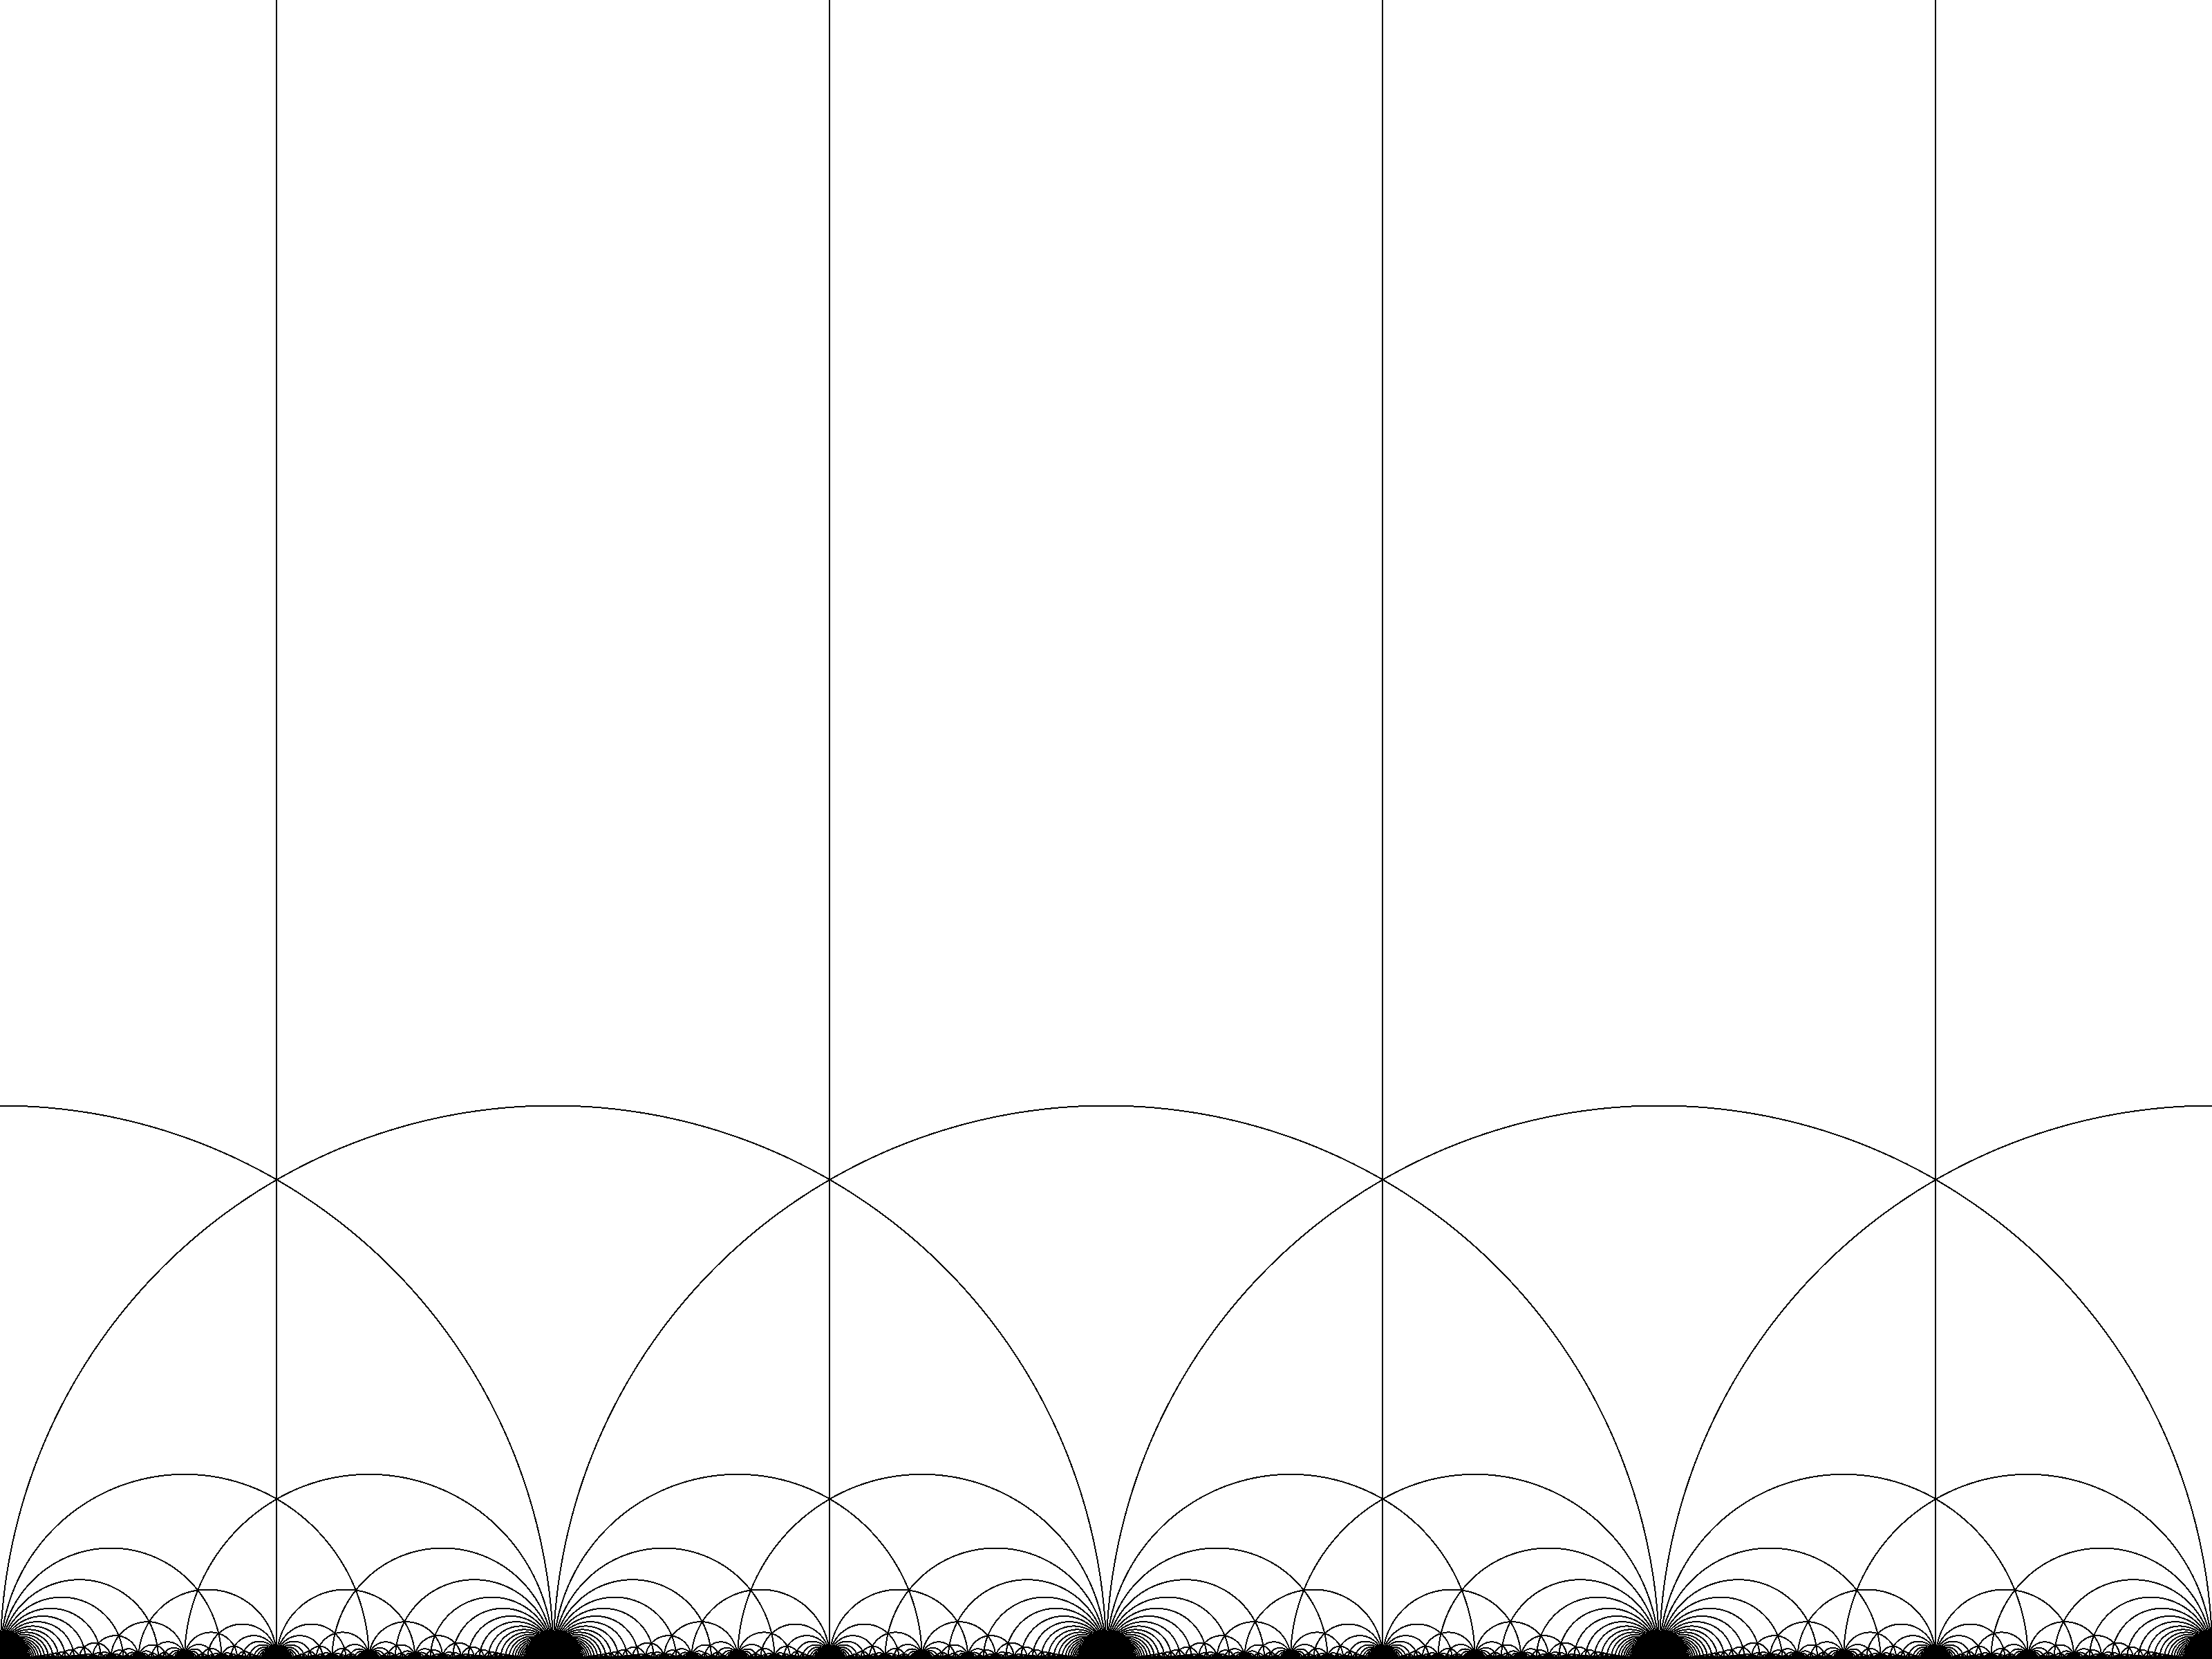
\includegraphics[scale=0.12]{ModularTiling_3.png}
    \caption{Delovanje modularne grupe $\SL$ na $\HH$.}
    \label{slika delovanja modularne grupe}
\end{figure}

Naslednja trditev pove, da vsaka orbita seka fundamentalno domeno vsaj v eni točki.

\begin{trditev}
    \label{predstavnik fundamentalne domene}
    Za vsak $z \in \HH$ obstaja $\gamma \in \SL$, da je $\gamma z \in D$.
\end{trditev}

\begin{dokaz}
    Spomnimo se identitete \eqref{eq: imginarni del delovanja}, ki nam pove kako se transformira imaginarni del kompleksnega števila, ko na njem delujemo z grupo $\SL$. Izraz $\abs{cz + d}$ meri razdalijo elementa $cz + d$ iz mreže $\lattice{1}{z}$ do izhodišča. Za dano konstanto $M > 0$ tako že vemo, da obstaja zgolj končno mnogo parov $(c,d) \in \Z^2$, da je $\abs{cz + d} < M$. V posebnem imamo torej tudi končno mnogo parov $(c,d)$ za katere sta $c$ in $d$ tuji, ki zadoščata tej oceni. Kadar sta $c$ in $d$ tuji namreč ravno ustrezata nekemu elementu $\gamma' \in \SL$, saj tedaj obstajata še $a,b \in \Z$, da velja $ad - bc = 1$. Za neki tak par $(c,d)$ \oz element $\gamma' \in \SL$, je vrednost izraza $\abs{cz + d}$ minimalna. Posledično je zato $\Im(\gamma' z)$ maksimalna.
    % lahko tudi več, je vrednost izraza $\abs{cz + d}$ minimalna in recimo, da je ta vrednost $\delta > 0$. Tedaj za vsak $\gamma \in \SL$ velja ocena
    % \[
    %     \Im(\gamma z) = \frac{\Im(z)}{\abs{cz + d}^2} \leq \frac{\Im(z)}{\delta^2}.  
    % \]
    Vzemimo enega izmed teh $\gamma' \in \SL$ pri katerem je $\Im(\gamma'z)$ maksimalna, in s $T$ delujmo na $\gamma'z$ tolikokrat, da bo za $z' = T^n\gamma'z$ veljalo
    \[
        -1/2 \leq \Re(z') \leq 1/2.
    \]
    To je vedno mogoče, saj delovanje z elementom $T$ predstavlja translacijo za eno enoto v pozitivni smeri realne osi. Ob tem še opomnimo, da takšne translacije s $T$ nimajo vpliva na imaginarni del, torej na koncu še vedno velja $\Im(z') = \Im(\gamma'z)$. 

    Če je tedaj $\abs{z'} \geq 1$, smo končali in lahko vzamemo $\gamma = T^n\gamma'$ za katerega velja $\gamma z\in D$. V nasprotnem primeru, če je $\abs{z'} < 1$, pa ugotovimo, da velja $\Im(Sz') = \frac{\Im(z')}{\abs{z}^2} > \Im(z')$
    % \[
    %     \Im\left(\frac{-1}{z'}\right) = \frac{\Im(z')}{\abs{z'}^2} > \Im(z')  
    % \]
    kar je v nasprotju z maksimalnostjo $\Im(z') = \Im(\gamma'z)$, torej do tega primera sploh ne pridemo.
\end{dokaz}


\begin{komentar}
    Z našo definicijo fundamentale domene $D$ zares ne dosežemo, da ta vsebuje \emph{enoličnega} predstavnika iz vsake orbite, saj nekatere točke na robu domene še vedno ležijo v isti orbiti. Imamo pa te vrste enoličnost v notranjosti domene $D$.
    % \emph{ne} vsebuje, po natanko enega predstavnika iz vsake orbite, saj so nekatere točke na njenem robu še vedno ekvivalentne. 
    Natančneje $z$ in $z'$ iz $D$ ležita v isti orbiti natanko tedaj, ko je $\abs{\Re(z)} = \frac12$ in $z = z' \pm 1$ ali pa je $\abs{z} = 1$ in je $z' = -1/z$. Dokaz najdemo v \cite[Izrek 1, VII, \S1]{Serre}.
\end{komentar}

Vrnimo se sedaj nazaj k mrežam oblike $\langle 1, \tau \rangle$, kjer je $\tau \in \HH$. Omenjali smo že, da sta mreži $\lattice{1}{\tau_1}$ in $\lattice{1}{\tau_2}$ homotetični, če med $\tau_1$ in $\tau_2$ lahko prehajamo z nekim zaporedjem delovanj $S$ in $T$. Naslednja trditev nam poda karakterizacijo homotetičnosti mrež preko grupe $\SL$.

% da imamo z grupo $\SL$ podano deobro definirano delovanje na zgornji polravnini $\HH$.

% do kolikšnje mere je ta izbira neenolična. 

% Zato, da ugotovimo mero neenoličnosti izbire tega $\tau$ 
% Tu se vplete \emph{specialna linearna grupa} 

\begin{trditev}
    \label{ekvivalentne normalizirane mreze}
    Naj bosta $\Lambda_1 = \langle 1, \tau_1 \rangle$ in $\Lambda_2 = \langle 1, \tau_2 \rangle$ mreži s $\tau_1, \tau_2 \in \HH$. Tedaj velja $\Lambda_1 \htp \Lambda_2$ natanko tedaj, ko obstaja $\gamma \in \SL$,  da je 
    \[
        \tau_1 = \gamma\tau_2.
    \]
\end{trditev}

\begin{dokaz}
    Denimo, da velja $\Lambda_1 \htp \Lambda_2$. Tedaj obstaja $\alpha \in \CM$, da je $\langle \alpha, \alpha\tau_1 \rangle = \langle 1, \tau_2 \rangle$. To pomeni, da lahko osnovni periodi $\alpha$ in $\alpha\tau_1$ izrazimo kot $\Z$-linearni kombinaciji $1$ in $\tau_2$, denimo 
    \[
        \alpha\tau_1 = a\tau_2 + b \quad \text{ in } \quad \alpha = c\tau_2 + d  
    \]
    za neke $a, b, c, d \in \Z$. Z drugimi besedami to pomeni, da obstaja celoštevilska obrnljiva matrika $\gamma = \abcd \in \GL_2(\Z)$, ki bazo $(1,\tau_1)$ preslika v bazo $(\alpha, \alpha\tau_2)$. Determinanta celoštevilske obrnljive matrike je lahko samo $1$ ali $-1$, ker pa velja 
    \[
        \Im\left(\frac{a\tau_2 + b}{c\tau_2 + d}\right) = 
        \frac{\Im(\tau_2)}{\abs{c\tau_2 + d}^2}> 0,
    \]
    mora biti $\det\gamma = 1$ \oz $\gamma \in \SL$ in $\tau_1 = \gamma\tau_2$.
    
    % s celoštevilskimi koeficienti, ki ohranja orientacijo in bazo $(\alpha, \alpha\tau_1)$ preslika na bazo $(1, \tau_2)$. Obrnljive matrike s celoštevilskimi koeficienti lahko imajo determinanto enako le $1$ ali $-1$, ker pa naša ohranja tudi orientacijo, mora biti njena determinanta enaka $1$. Od tod je $ad - bc = 1$ in $\tau_1 = \frac{a\tau_2 + b}{c\tau_2 + d} = \gamma.\tau_2$, za $\gamma = \abcd \in \SL$.

    Obratno, če velja $\tau_1 = \gamma\tau_2$, za neki $\gamma = \abcd \in \SL$, imamo
    \[
        \lattice{1}{\tau_1} = 
        \lattice{1}{\tfrac{a\tau_2 + b}{c\tau_2 + d}} \htp
        \lattice{c\tau_2 + d}{a\tau_2 + b},
    \]
    preko homotetije, ki jo porodi množenje s številom $\alpha = c\tau_2 + d$. Ker je $\Im\tau_2 > 0$, je $\alpha$ res neničelen. Opazimo, da je mreža $\lattice{c\tau_2 + d}{a\tau_2 + b}$ kar enaka $\lattice{1}{\tau_2}$, saj lahko njeni osnovni periodi $1$ in $\tau_2$ izrazimo kot $\Z$-linearni kombinaciji osnovnih period $a\tau_2 + b$ in $c\tau_2 + d$:
    \begin{gather*}
        a(c\tau_2 + d) - c(a\tau_2 + b) = ad - bc = 1, \\
        d(a\tau_2 + b) - b(c\tau_2 + d) = (ad - bc)\tau_2 = \tau_2.
    \end{gather*}
    Ker je $\gamma \in \SL$, smo upoštevali $ad - bc = 1$. Tako dobimo $\lattice{1}{\tau_1} \htp \lattice{1}{\tau_2}$.
\end{dokaz}

Zgornja diskusija o fundamentalni domeni $D$ in prejšnja trditev nam tako povesta, da lahko vsaki mreži $\Lambda \subseteq \C$ priredimo točko $\tau \in D$ iz fundamentalne domene, da je $\Lambda \htp \lattice{1}{\tau}$.

\subsubsection{Modularne funkcije}

\begin{definicija}
    Naj bo $k$ celo število. Meromorfna funkcija $f$ na zgornji polravnini $\HH$ je \emph{šibko modularna reda $2k$}, če zadošča \emph{modularnostnem pogoju}
    % \ti \emph{modularnemu pogoju}: za vse $z \in \HH$ in $\gamma \in \SL$ velja
    \begin{equation}
        \label{eq: modularnostni pogoj}
        f(z) = (cz + d)^{-2k} f\left(\frac{az + b}{cz + d}\right) \quad \text{za vse } \pabcd \in \operatorname{SL}_2(\Z).
    \end{equation}
    % Zvezi \eqref{eq: modularnostni pogoj} pravimo \emph{modularnostni pogoj.} 
    Če dodatno obstaja limita $f$ v neskončnosti (v posplošenem smilsu -- dovoljujemo tudi konvergenco proti $\infty$), pravimo, da je $f$ \emph{modularna funkcija reda $2k$}. 
\end{definicija}

\begin{opomba}
    Matriki $S = \big(\begin{smallmatrix} 0 & -1\\1 & 0 \end{smallmatrix}\big)$ in $T = \big(\begin{smallmatrix} 1 & 1\\0 & 1 \end{smallmatrix}\big)$ generirata grupo $\operatorname{SL}_2(\Z)$, zato se modularnostni pogoj prepiše v ekvivalentnega
    \[
        f(z) = z^{-2k}f\left(-1/z\right) \quad \text{ in } \quad f(z) = f(z + 1),
    \] 
    za vse $z \in \HH$, od koder vidimo, da so vse (šibko) modularne funkcije v posebnem tudi periodične s periodo $1$.
\end{opomba}

\begin{opomba}
    % V resnici smo definirali samo šibko modularne funkcije sodih redov. Izkaže se, da neničelnih šibko modularnih funkcij lihih redov spolh ni. Če bi $f$ bila takšna, za $\gamma = \big(\begin{smallmatrix} -1 & 0\\0 & -1 \end{smallmatrix}\big)}$ velja
    Definicija namiguje, da šibko modularnih funkcij lihega reda reda sploh ni in izkaže se, da je to res, če ob tem izvzamemo ničelno funkcijo. Če bi namreč $f$ bila lihega reda, za $\gamma = -I \in \operatorname{SL}_2(\Z)$ velja
    \[
        f(z) = (-1)^{2k+1}f(\gamma z) = -f(z) \quad \text{ za vse } z \in \HH,
    \]
    od koder sledi $f=0$.
\end{opomba}

\subsubsection*{Eisensteinove vrste}
Zanenkrat nimamo še nobenih konkretnih primerov (šibko) modularnih funkcij, razen konstant. Videli pa bomo, da bodo Eisensteinove vrste reda $2k$, kjer je $k > 1$, prirejene mreži $\Lambda$
\[
    G_{2k}(\Lambda) = \sum_{\om\in\Lambda'}\frac{1}{\om^{2k}},
\]
služile kot dober vir za konstrukcijo prvih netrivialnih primerov modularnih funkcij. V ta namen si poglejmo naslednjo trditev.

\begin{trditev}
    Naj bo $\Lambda$ mreža v $\C$ in $\alpha \in \CM$. Tedaj velja
    \begin{equation}
    \label{eq: transformacija G_k vrst}
        G_{2k}(\alpha\Lambda) = \alpha^{-2k}G_{2k}(\Lambda)
    \end{equation}
\end{trditev}

\begin{dokaz}
    Identiteto pokažemo z računom
    \[
        G_{2k}(\alpha\Lambda) = \sum_{\om\in\Lambda'}\frac{1}{(\alpha\om)^{2k}} = \alpha^{-2k}\sum_{\om\in\Lambda'}\frac{1}{\om^{2k}} = \alpha^{-2k}G_{2k}(\Lambda). \qedhere
    \]
\end{dokaz}
Za poljuben $\tau \in \HH$ imamo mrežo $\lattice{1}{\tau}$ na kateri lahko izračunamo vrsto $G_{2k}$. Tako dobimo funkcijo, ki jo označimo enako, podano s predpisom
\[
    G_{2k} : \HH \to \C, \quad G_{2k}(\tau) = \sum_{(m,n) \in \Z^2\setminus\{0\}} \frac{1}{(m + n\tau)^{2k}}.
\]
Naj bo $\gamma \in \SL$ poljuben. Homotetični mreži $\lattice{1}{\tau}$ in $\lattice{1}{\gamma\tau}$, kot v dokazu trditve \ref{ekvivalentne normalizirane mreze}, povezuje $\alpha = c\tau + d$, da velja
\[
    \lattice{1}{\tau} = \alpha\lattice{1}{\tfrac{a\tau + b}{c\tau + d}}.
\]
Preko zveze \eqref{eq: transformacija G_k vrst} lahko tako izpeljemo modularnostni pogoj za funkcijo $G_{2k}$
\[
    G_{2k}(\tau) = (c\tau + d)^{-2k}G_{2k}\left(\frac{a\tau + b}{c\tau + d}\right).
\]
Nekoliko tehničen dokaz
% , ki ga najdemo v dodatku \ref{}, 
nam pokaže še, da so funkcije $G_{2k} : \HH \to \C$ tudi holomorfne.

\begin{trditev}
    \label{holomorfnost Gk}
    Naj bo $k \in \N$. Eisensteinova vrsta reda $2k$ s predpisom $G_{2k}(\tau) = G_{2k}(\lattice{1}{\tau})$ podaja holomorfno funkcijo $\HH \to \C$ na zgornji polravnini.
    % $\Lambda_\tau = \langle 1, \tau \rangle$
    % \[
    %     G_k(\Lambda) = G_k(\langle 1, \tau \rangle) = 
    %     \sum_{(m,n) \in \Z^2\setminus\{0\}} \frac{1}{(m + n\tau)^k}  
    % \]
    % podaja holomorfno funkcijo na zgornji polravnini $\tau \in \HH$, z isto oznako
    % \[
    %     G_k : \HH \to \C, \quad G_k(\tau) = G_k(\langle 1, \tau \rangle).
    % \]
\end{trditev}

\begin{dokaz}
    Zaradi Weierstrassovega M-testa in izreka \ref{izrek o konvergenci holomorfnih funkcij} zadošča vsak člen vrste $G_{2k}$ po kompaktih v $\HH$ majorizirati s členom neke konvergentne vrste. Če je $K \subseteq \HH$ poljuben kompakt, obstajata taka $a, \varepsilon > 0$, da je $K$ vsebovan v množici 
    \[
        S_{a,\epsilon} = \{z \in \HH \mid \abs{\Re(z)} \leq a \text{, } \Im(z) \geq \varepsilon \}.
    \]
    Izkaže se, da obstaja tak $\delta \in (0,1)$, za katerega je
    \begin{equation}
        \label{eq: ocena za holomorfnost eisensteinove vrste}
        \abs{m + n\tau} \geq \delta\abs{m + ni},  
    \end{equation}
    za vse $(m, n) \in \Z^2\setminus\{0\}$ in vse $\tau \in S_{a,\varepsilon}$. To oceno uporabimo na kompaktu $K$ za majorizacijo vsakega od členov vrste $G_{2k}(\tau)$ na sledeč način
    \[
        \frac{1}{\abs{m + n\tau}^{2k}} \leq \delta^{-2k}\frac{1}{\abs{m + ni}^{2k}}.
    \]
    % \[
    %     \sum_{(m,n) \in \Z^2\setminus\{0\}} \frac{1}{\abs{m + n\tau}^k}
    %     \leq \sum_{(m,n) \in \Z^2\setminus\{0\}} \frac{1}{\delta^k \abs{m + ni}^k}
    %     = \frac{1}{\delta^k} \sum_{(m,n) \in \Z^2\setminus\{0\}} \frac{1}{\abs{m + ni}^k}.
    % \]
    Zadnje predstavlja ravno s konstanto pomnožen člen absolutno konvergentne vrste $G_{2k}(\lattice{1}{i})$, zato je $G_{2k}$ res holomorfna na $\HH$.

    % Zadnja vrsta predstavlja ravno $G_k(\langle 1, i \rangle)$, ki je po lemi \ref{lema o konvergenci eisensteinove vrste} absolutno konvergentna, torej je $G_k$ res holomorfna funkcija na zgornji polravnini.

    Vrnimo se sedaj še k oceni \eqref{eq: ocena za holomorfnost eisensteinove vrste}. Če je $n = 0$, ocena drži za katerikoli $\delta < 1$, zato bo ekvivalentno pokazati obstoj takega $\delta \in (0,1)$, da bo za vse $(m,n) \in \Z^2$, kjer je $n \neq 0$, in $\tau \in S_{a,\varepsilon}$ veljalo
    \[
        \abs{\frac{\tau + \tfrac{m}{n}}{i + \tfrac{m}{n}}} \geq \delta.
    \]
    Definirajmo funkcijo $f: S_{a, \varepsilon} \times \R \to (0,\infty)$ s predpisom $f(\tau, x) = \abs{\tfrac{\tau - x}{i - x}}$. Za vsak fiksen $\tau$, velja $\lim_{x \to \pm\infty} f(\tau, x) = 1$, torej obstaja $R_\tau > 0$, da je $\abs{\tfrac{\tau - x}{i - x}} \geq \tfrac{1}{2}$ za vse $\abs{x} \geq R_\tau$. Hkrati pa zaradi zveznosti, funkcija $f$ na kompaktu $\{\tau\} \times [-R_\tau, R_\tau]$ doseže minimum $c_\tau > 0$. Tedaj zadošča vzeti $\delta_\tau = \min\{c_\tau, \tfrac{1}{2}\}$, za katerega je $f(\tau, x) \geq \delta_\tau$.

    To oceno izpeljimo še enakomerno glede na $\tau$. Za poljuben $\tau \in S_{a, \varepsilon}$ in $x > a$ velja 
    \[
        \abs{\frac{\tau - x}{i - x}} \geq \abs{\frac{a + i\varepsilon - x}{i - x}},
    \]
    kot vidimo na sliki \ref{mnozica S_a,eps}, torej bo za vse $\tau \in S_{a, \varepsilon}$ in vse $x > a$
    % $x > \max\{R_{a + i\varepsilon}, a\} = r_+$
    veljalo $\abs{\tfrac{\tau - x}{i - x}} \geq \delta_{a+i\varepsilon}$. 
    \begin{figure}
        \centering
        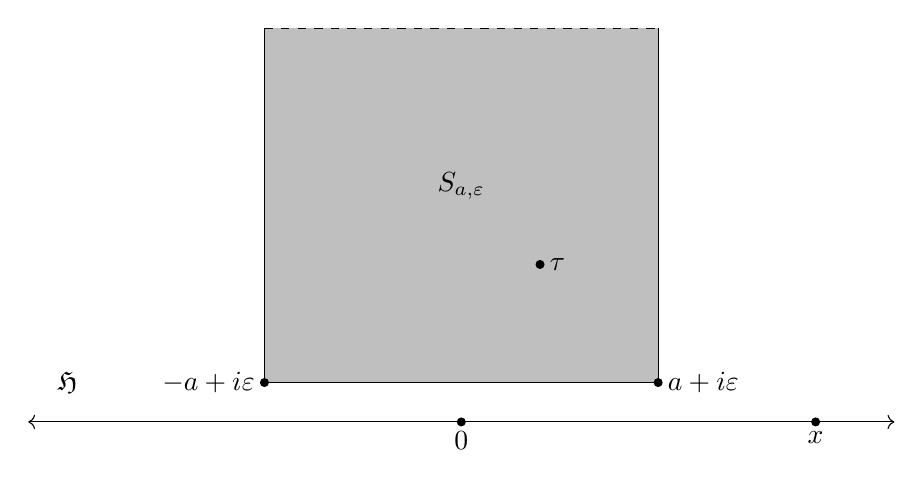
\begin{tikzpicture}
            \begin{scope}
                % \clip (0,0) rectangle (14cm, 5cm);
                \fill[fill = gray!50] (0,0.5) rectangle (5,5);
                \draw (2.5,3) node {$S_{a,\varepsilon}$};
                \draw[<->] (-3, 0) -- (8,0);
                \draw[dashed] (0,5) -- (5,5);
                \draw (0,0.5) -- (5,0.5);
                \draw (0,0.5) -- (0,5);
                \draw (5,0.5) -- (5,5);
                \draw (2.5,0) node [below]{$0$};
                \node[draw,circle,inner sep=1pt,fill] at (2.5,0) {};
                % \draw (5,0) node [below]{$a$};
                % \node[draw,circle,inner sep=1pt,fill] at (5,0) {};
                % \draw (0,0) node [below]{$-a$};
                % \node[draw,circle,inner sep=1pt,fill] at (0,0) {};
                \draw (0,0.5) node [left]{$-a + i\varepsilon$};
                \node[draw,circle,inner sep=1pt,fill] at (0,0.5) {};
                \draw (5,0.5) node [right]{$a + i\varepsilon$};
                \node[draw,circle,inner sep=1pt,fill] at (5,0.5) {};
                \draw (3.5,2) node [right]{$\tau$};
                \node[draw,circle,inner sep=1pt,fill] at (3.5,2) {};
                \draw (7,0) node [below]{$x$};
                \node[draw,circle,inner sep=1pt,fill] at (7,0) {};
                \draw (-2.5,0.25) node [above]{$\HH$};
            \end{scope}
        \end{tikzpicture}

        \caption{Množica $S_{a,\varepsilon}$ v zgornji polravnini $\HH$.}
        \label{mnozica S_a,eps}
    \end{figure}
    %    
    Simetrično lahko sklepamo, da bo $\abs{\tfrac{\tau - x}{i - x}} \geq \delta_{-a+i\varepsilon}$ za vse $\tau \in S_{a, \varepsilon}$ in vse $x < -a$. Za $x \in [-a,a]$ in vse $\tau \in S_{a, \varepsilon}$ pa velja $\abs{\frac{\tau - x}{i - x}} \geq \frac{\varepsilon}{\abs{i - x}} \geq \frac{\varepsilon}{\abs{i - a}}$.
    Skupaj je torej 
    \[
        \abs{\frac{\tau - x}{i - x}} \geq \delta, \quad \text{ za vse } \tau \in S_{a, \varepsilon} \text{ in vse } x \in \R,
    \]
    kjer za $\delta$ vzamemo $\delta := \min\{\delta_{a + i\varepsilon}, \delta_{-a + i\varepsilon}, \frac{\varepsilon}{\abs{i - a}}\} \in (0,1)$, kar zaključi dokaz. \qedhere 
    % $\abs{\frac{\tau - x}{i - x}} \geq \delta$ za vse $x \in \R$ ter $\tau \in S_{a,\varepsilon}$, kjer za $\delta$ vzamemo $\delta := \min\{\delta_{a + i\varepsilon}, \delta_{-a + i\varepsilon}, \frac{\varepsilon}{\abs{i - a}}\} \in (0,1)$.  
    
    % $x < \min\{-R_{-a + i\varepsilon}, -a\} = r_-$. 
    % Zaradi zveznosti, $f$ doseže minimalno vrednost $c > 0$ na kompaktu $S_{a, \varepsilon} \times [r_-, r_+]$, torej nazadnje, za $\delta = \min\{c, \tfrac{1}{2}\} > 0$ dobimo 
    % \[
    %     \abs{\frac{\tau - x}{i - x}} \geq \delta, \quad \text{ za vse } \tau \in S_{a, \varepsilon} \text{ in vse } x \in \R,
    % \]
    % kar zaključi dokaz.
\end{dokaz}


% in tako nam ta družina funkcij podaja prvi netrivialen primer šibko modularnih funkcij reda $2k$. 

Pomembna lastnost funkcij $G_{2k}$, ki bo tudi precej koristna, je njihovo obnašanje v neskončnosti. Naj $\zeta(s) = \sum_{n = 1}^\infty n^{-s}$ označuje \emph{Riemannovo $\zeta$-funkcijo}, kjer je $\Re(s) > 1$. Tedaj imamo trditev.

\begin{trditev}
    \label{G2k v neskoncnosti}
    Za funkcije $G_{2k}$ obstaja limita v neskončnosti, ki je končna in enaka 
    \[
        \lim_{\tau \to \infty}G_{2k}(\tau) = 2\zeta(2k).  
    \]
\end{trditev}

\begin{dokaz}
    Izračunajmo limito preko zaporedji. Naj bo $(z_\ell)_{\ell\in\N}$ poljubno zaporedje v zgornji polravnini $\HH$, ki konvergira proti $\infty$\footnote{Zaporedje $(z_n)_{n \in \N}$ \emph{konvergira} proti $\infty$, kadar za vsak $M > 0$ obstaja $n_0 \in \N$, da za vse $n \in \N$, za katere je $n \geq n_0$, velja $\abs{z_n} > M$.}. Ker $G_{2k}$ zadošča modularnostnemu pogoju, je v posebnem invariantna na translacije s $T$, zato lahko brez škode za splošnost predpostavimo, da za vsak člen zaporedja velja $-\frac12 \leq \Re(z_\ell) \leq \frac12$. Poleg tega, zaradi konvergence proti $\infty$, obstaja $\varepsilon > 0$, da je $\Im(z_\ell) > \varepsilon$ za vse $\ell \in \N$.  Tako smemo predpostaviti, da zaporedje $(z_\ell)_{\ell \in\N}$ leži v množici $S_{1/2, \varepsilon}$. Iz dokaza trditve \ref{holomorfnost Gk} vemo, da $G_{2k}$ na množicah te oblike konverigra enakomerno, torej lahko zamenjamo limiti
    \begin{gather*}
        \lim_{\ell \to \infty}G_{2k}(z_\ell) = 
        \sum_{(m,n) \in \Z^2\setminus\{0\}} \lim_{\ell \to \infty} \frac{1}{(m + nz_\ell)^{2k}} = 
        % \sum_{m \in \Z\setminus\{0\}} \frac{1}{m^4} = 
        2 \cdot \sum_{m = 1}^\infty \frac{1}{m^{2k}} = 2\zeta(2k),
    \end{gather*}
    kar da želeni rezultat.
\end{dokaz}

Tako družina funkcij $G_{2k}$ podaja prvi netrivialen primer modularnih funkcij redov $2k$, za vsa naravna števila $k$.


\subsubsection*{Modularna diskriminanta}
Iz definicije je razvidno, da je množica šibko modularnih funkcij danega reda $2k$ zaprta za $\C$-linearne kombinacije, torej tvori kompleksen vektorski prostor. Na ta način lahko iz starih šibko modularnih funkcij reda $2k$ dobimo nove, ki so spet reda $2k$. Pomembna konstrukcija, ki nam omogoča prehajanje med različnimi redi, pa je produkt. Če sta $f_1$ in $f_2$ šibko modularni reda $2k_1$ in $2k_2$, je njun produkt $f_1f_2$ šibko modularna funkcija reda $2k_1 + 2k_2$. To sledi iz modularnostenga pogoja, ki mu zadošča $f_1f_2$. Za vsak $\gamma \in \operatorname{SL}_2(\Z)$ namreč velja
\begin{align*}
    f_1(z)f_2(z) &= 
    (cz + d)^{-2k_1} f_1\left(\gamma z\right)(cz + d)^{-2k_2} f_2\left(\gamma z\right) \\
    &= (cz + d)^{-2k_1 - 2k_2} f_1f_2\left(\gamma z\right).
\end{align*}
Kompleksen vektorski prostor vseh šibko modularnih funkcij tako postane kompleksna algebra z enoto, ki je konstantna funkcija $1$ reda $0$.

Spomnimo se oznak $g_2(\Lambda) = 60G_4(\Lambda)$ in $g_3(\Lambda) = 140G_6(\Lambda)$ iz poglavja \ref{elipticne funkcije}. Povsem analogno definiramo modularni funkciji
\[
    g_2(\tau) = 60G_4(\tau) \quad \text{ in } \quad g_3(\tau) = 140G_6(\tau)
\]
redov $4$ in $6$. Iz njiju lahko konstruiramo \emph{modularno diskriminanto}
\[
    \Delta = g_2^3 - 27g_3^2,
\]
ki je šibko modularna funkcija reda $12$. Poleg tega $\Delta$ nima ničle na zgornji polravnini $\HH$, kot smo preko mrež in Weierstrassove $\wp$-funkcije videli v dokazu trditve \ref{nenicelna diskriminanta}. Trditev \ref{G2k v neskoncnosti} pa nam omogoči sklepati še o njeni limiti v neskončnosti, ki je 
\[
    \lim_{\tau \to \infty} \Delta(\tau) = 0.
\]
Pri tem smo uporabili poznani vrednosti $\zeta(4) = \frac{\pi^4}{2\cdot3^3\cdot5}$ in $\zeta(6) = \frac{\pi^6}{3^3\cdot5\cdot7}$, ki ju lahko izračunamo s pomočjo Fourierovih vrst in Parsevalove enakosti, ali pa se skličemo na \cite[VII, \S4.1]{Serre}, za izračun limit
\begin{align*}
    &\lim_{\tau \to \infty} g_2(\tau) = 60\cdot2 \zeta(4) = \frac{4\pi^4}{3},\\
    &\lim_{\tau \to \infty} g_3(\tau) = 140\cdot2 \zeta(6) = \frac{8\pi^6}{27}.
\end{align*}

\subsubsection*{Modularna $j$-invraianta} Celotna razprava o modularnih funkcijah nas na koncu privede še do \emph{modularne $j$-invariante}. V osnovi je $j$-invarianta število 
\[
    j = 1728\frac{a^3}{a^3 - 27b^2}
\]
prirejeno eliptični krivulji z enačbo $y^2z = 4x^3 - axz^2 - bz^3$, kjer je $a^3 - 27b^2 \neq 0$. Nad poljem kompleksnih števil nam je $j$-invarianta omogočila karakterizirati vse projektivne kubike do projektivne ekvivalence natančno. Na podoben način tedaj vpeljemo \emph{modularno $j$-invarianto}, podano s predisom
\[
    j(\tau) = 1728\frac{g_2(\tau)^3}{\Delta(\tau)}
    = 1728\frac{g_2(\tau)^3}{g_2(\tau)^3 - 27g_3(\tau)^2}.
\]
Funkcija $j$ je holomorfna na $\HH$, saj sta takšni že $g_2^3$ in $\Delta$, slednja pa na $\HH$ nima ničle. Poleg tega sta $g_2^3$ in $\Delta$ modularni funkciji in obe sta reda $12$. Od tod sledi, da je $j$ modularna funkcija reda $0$, kar pomeni, da delovanje grupe $\SL$ na njenem argumentu nima vpliva na njeno vrednost -- na vsaki $\SL$-orbiti delovanja je $j$ konstantna. Njena limita v neskončnosti je 
\[
    \lim_{\tau \to \infty}j(\tau) = \infty,
\]
kar je razvidno iz obnašanja funkcij $g_2$ in $\Delta$ v neskončnosti. Vse skupaj lahko povzamemo v trditvi.

\begin{trditev}
    Funkcija $j : \HH \to \C$ je modularna funkcija reda $0$ z limito v neskončnosti $\lim_{\tau \to \infty}j(\tau) = \infty$.
\end{trditev}

\begin{komentar}
    Kot vsaka modularna funkcija, tudi $j$ zadošča zvezi $j(\tau) = j(\tau + 1)$, torej je periodična. Ker je tudi holomorfna, jo lahko razvijemo v nekakšno Fourierovo vrsto. Če pišemo $q = e^{2\pi i \tau}$, se izkaže, da velja
    \[
        j(\tau) = \frac{1}{q} + 744 + 196884q + 21493760q^2 + \cdots.
    \]
    Vrsto te oblike imenujemo tudi \emph{$q$-razvoj}. Število $1728$ v predpisu za $j$ je tradicionalno in je najmanjše pozitivno število, ki zagotovi celoštevilskost koeficientov $q$-razvoja $j$-invariante. O tem lahko več izvemo v \cite[VII, \S3]{Serre}.
\end{komentar}

% Če se osredotočimo na fundamentalna paralelograma obeh mrež, bosta ta dva homotetična natanko tedaj, ko bosta pripadajoči mreži homotetični. Še ena interpretacija te ekvivalence pa vpleta razmerji dolžin njunih stranic. Središčni raztegi in rotacije ravno ohranjajo to razmerje, torej bosta dve mreži homotetični natanko tedaj, ko bosta imala enaki razmerji dolžin njunih stranic. 

% To nas privede do vpeljave nekakšne standardne oblike mreže, kjer zahtevamo, da je ena od osnovnih period enaka $1$. Za poljubno mrežo $\Lambda$ lahko izberemo osnovni periodi $\om_1$ in $\om_2$, za kateri velja $\Lambda = \langle \om_1, \om_2 \rangle$. Dodatno smemo privzeti, da je $\Im(\om_2/\om_1) > 0$, saj v nasprotnem primeru zamenjamo vlogi $\om_1$ in $\om_2$, kar se odraža v spremembi predznaka neničelne vrednosti $\Im(\om_2/\om_1)$. Tako imamo 
% \[
%     \langle \om_1, \om_2 \rangle \htp \langle 1, \om_2/\om_1 \rangle,
% \]
% preko homotetije, ki jo predstavlja množejne z $\om_1\inv \in \CM$.

% Naj $\Lattice$ označuje množico vseh mrež v kompleksni ravnini.

% \newpage

\subsection{Izomorfizem \texorpdfstring{$\C/\Lambda \to E(\C)$ in uniformizacija}{}} 

V tem razdelku podamo izomorfizem Riemannovih ploskev -- kompleksnega torusa $\torus$ in eliptične krivulje $E_\Lambda$, podane z enačbo
\[
    y^2z = 4x^3 - g_2(\Lambda)xz^2 - g_3(\Lambda)z^3.
\]
Nazanje s pomočjo modularne $j$-invariante dokažemo še uniformizacijo, ki opisuje, kako poljubni eliptični krivulji nad $\C$ priredimo mrežo $\Lambda$ in posledično izomorfen kompleksni torus $\torus$.

\begin{izrek}
    \label{izomorfizem torusa in krivulje}
    Naj bo $\Lambda \subseteq \C$ mreža, $\wp$ Weierstrassova eliptična funkcija glede na to mrežo $\Lambda$ in naj bo $E(\C)\subseteq \PC$ eliptična krivulja podana z enačbo
    \[
        E: \quad y^2z = 4x^3 - g_2(\Lambda)xz^2 - g_3(\Lambda)z^3.  
    \]
    Tedaj je preslikava $\phi : \torus \to E(\C)$ podana s predpisom
    \[
        z + \Lambda \mapsto 
        \begin{cases}
            \pcoor{\wp(z) : \wp'(z) : 1}; \quad &z \not\in \Lambda \\
            \oio; \quad &z \in \Lambda
        \end{cases}  
    \]
    dobro definiran biholomorfizem Riemannovih ploskev.
\end{izrek}

\begin{dokaz}
    Razdelimo dokaz trditve na naslednje štiri dele: dobro definiranost, zveznost, bijektivnost in holomorfnost preslikave $\phi$.
    \subsubsection*{Dobra definiranost}
    % Najprej se lotimo dobre definiranosti preslikeve $\phi$. 
    Po izreku \ref{ode za wp} za poljuben $z \in \C\setminus\Lambda$ velja $\pcoor{\wp(z) : \wp'(z) : 1} \in E(\C)$ in posebej je tudi $\oio \in E(\C)$, torej bo slika preslikave $\phi$ res vsebovana v eliptični kriulji $E(\C)$. 
    
    Predpis za $\phi$ je podan na kvocientu $\torus$, torej se moramo prepričati še o neodivisnosti le tega od izbire predstavnikov ekvivalenčnih razredov. Če sta $z,w \in \C$ predstavnika istega ekvivalenčnega razreda, velja $z - w \in \Lambda$ \oz $w = z + \om$, za neki $\om \in \Lambda$. V primeru, ko je $z \not\in \Lambda$, je tudi $w \not\in \Lambda$, in tedaj zaradi $\Lambda$-periodičnosti funkcije $\wp$ velja
    \[
        \pcoor{\wp(w) : \wp'(w) : 1} = 
        \pcoor{\wp(z + \om) : \wp'(z  + \om) : 1} =
        \pcoor{\wp(z) : \wp'(z) : 1}. 
    \]
    Kadar pa sta $z, w \in \Lambda$, je že sam predpis $\phi$ neodvisen od izbire predstavnika, torej je celoten predpis $\phi$ res dobro definiran na točkah kvocienta $\torus$. 

    \subsubsection*{Zveznost}
    % Naslednje se bomo prepričali, da je preslikava $\phi: \torus \to E(\C)$ zvezna. 
    Za nadaljevanje bo koristno poznati limiti
    \[
        \lim_{z \to 0} \frac{\wp(z)}{\wp'(z)} = 0 \quad \text{in} \quad 
        \lim_{z \to 0} \frac{1}{\wp'(z)} = 0,
    \] 
    zato ju izračunajmo. Spomnimo se obnašanja $\wp$ \oz $\wp'$ okoli svojih polov. Po trditvi \ref{lastnosti wp} ima $\wp$ v točki $0$ pol druge stopnje, zato obstajata takšni holomorfni funkciji $g,h \in \hol{U}$, definiranih na neki dovolj majhni odprti okolici $U\subseteq\C$ točke $0$, ki sta na $U$ neničelni, da velja $\wp(z) = \frac{g(z)}{z^2}$ in $\wp'(z) = \frac{h(z)}{z^3}$ za vse $z \in U$. Tedaj izračunamo
    \[
        \lim_{z \to 0} \frac{\wp(z)}{\wp'(z)} = \lim_{z \to 0} \frac{g(z)z^3}{h(z)z^2} = 
        \frac{g(0)}{h(0)} \cdot \lim_{z \to 0}\frac{z^3}{z^2} = 0
    \]
    ter
    \[
        \lim_{z \to 0} \frac{1}{\wp'(z)} = \lim_{z \to 0} \frac{z^3}{h(z)} = 
        \frac{1}{h(0)} \cdot \lim_{z \to 0}z^3 = 0.
    \]
    Zaradi $\Lambda$-periodičnosti, dobimo tudi $\lim_{z \to \om} \frac{\wp(z)}{\wp'(z)} = 0$ in $\lim_{z \to \om} \frac{1}{\wp'(z)} = 0$ za vsak $\om \in \Lambda$. Vidimo torej, da imata funkciji $\frac{\wp}{\wp'}$ in $\frac{1}{\wp'}$ zgolj odpravljivi singularnosti v točkah iz $\Lambda$, kar pomeni, da ju lahko z vrednostjo $0$ v teh točkah holomorfno razširimo. Z manjšo zlorabo oznak bomo ti dve razšitivi spet označili kar s $\frac{\wp}{\wp'}$ oziroma $\frac{1}{\wp'}$ in razumeli $\frac{\wp(\om)}{\wp'(\om)} = 0$ ter $\frac{1}{\wp'(\om)} = 0$ za $\om \in \Lambda$.

    Po lemi \ref{polperiode so nicle odvoda wp} vemo, da ima $\wp'$ po tri enostavne ničle na fundamentalnem paralelogramu v polperiodah mreže $\Lambda$, \tj v množici $\frac{1}{2}\Lambda = \{\frac{\om}{2} \in \C \mid \om \in \Lambda\}$. 
    % Natančneje je množica ničel funkcije $\wp'$ natanko $\frac12\Lambda \setminus \Lambda$, v vsaki periodi iz mreže $\Lambda$ ima $\wp'$ namreč pole tretje stopnje. 
    Natančneje je množica ničel funkcije $\wp'$ natanko $\frac12\Lambda \setminus \Lambda$. Polperiode iz mreže $\Lambda$ smo izvzeli, saj ima v vsaki izmed njih $\wp'$ pol tretje stopnje. 
    Funkciji $\frac{\wp}{\wp'}$ in $\frac{1}{\wp'}$ lahko torej vidimo, kot dobro definirani holomorfni $\Lambda$-periodični funkciji na odprti domeni $\C \setminus (\frac12\Lambda \setminus \Lambda)$. 

    
    Naj $\pi : \C \to \torus$ označuje kvocientno projekcijo. Opazimo, da je $\phi$ natanko preslikava, ki se faktorizira skozi preslikavo
    \[
        \Phi: \C \to E(\C), \quad z \mapsto
        \begin{cases}
            \pcoor{\wp(z) : \wp'(z) : 1}; \quad &z \not\in \Lambda \\
            \oio; \quad &z \in \Lambda
        \end{cases}, 
    \]
    zato bo zaradi trditve \cite[trditev 3.22]{MrcunTop} dovolj preveriti zveznost $\Phi$, ker je $\pi$ kvocientna. Podali bomo dva predpisa za $\Phi$, definirana na odprtih podmnožicah v $\C$, katerih unija bo pokrila $\C$, in oba predpisa se bosta na njunem preseku ujemala. 
    
    Vzemimo odprti množici $U_0 = \C \setminus \Lambda$ in $U_1 = \C \setminus (\frac12\Lambda \setminus \Lambda)$ in definirajmo preslikavi
    \begin{gather*}
        \Phi_0 : U_0 \to E(\C), \quad z \mapsto \pcoor{\wp(z) : \wp'(z) : 1}, \\
        \Phi_1 : U_1 \to E(\C), \quad z \mapsto \pcoor{\tfrac{\wp(z)}{\wp'(z)} : 1 : \tfrac{1}{\wp'(z)}}.
    \end{gather*}
    Zaradi omenjenih lastnosti $\tfrac{\wp}{\wp'}$ in $\tfrac{1}{\wp'}$ sta $\Phi_0$ in $\Phi_1$ zvezni kot kompoziciji preslikav $\C \to \C^3\setminus\{0\}$ in zvezne kvocientne projekcije $q:\C^3\setminus\{0\} \to \PC$. Na preseku njunih domen $U_0 \cap U_1 = \C \setminus \frac12\Lambda$ velja
    \[
        \Phi_0(z) = \pcoor{\wp(z) : \wp'(z) : 1} = 
        \pcoor{\tfrac{\wp(z)}{\wp'(z)} : 1 : \tfrac{1}{\wp'(z)}} = \Phi_1(z),
    \]
    saj je $\wp'(z) \in \CM$ za $z \in \C \setminus \frac12\Lambda$. Ker preslikavi $\Phi_0$ in $\Phi_1$ skupaj določata ravno $\Phi$, je slednja zvezna, od koder sledi, da je tudi $\phi$ zvezna.  
     
% % -----------------
%     \newpage
%     Podali bomo alternativen predpis, definiran na dveh odprtih podmnožicah v $\torus$, ki se bo ujemal na njunem preseku. Naj $\pi : \C \to \torus$ označuje kvocientno projekcijo.
    
%     Zvezna preslikava 
%     \[
%         \C\setminus \Lambda \to \C^3\setminus\{0\}, \quad z \mapsto (\wp(z), \wp'(z), 1)
%     \]
%     zaradi $\Lambda$-periodičnosti $\wp$ in $\wp'$ inducirata zvezno preslikavo $\pi(\C \setminus \Lambda) \to \C^3\setminus\{0\}$ po trditvi \cite{MrcunTop}. Kompozicija slednje z zvezno kvocientno projekcijo $\C^3\setminus\{0\} \to \PC$ je zvezna s predpisom
%     \begin{equation}
%         \label{eq: prvi predpis izomorfizma}
%         z + \Lambda \mapsto \pcoor{\wp(z) : \wp'(z) : 1)},
%     \end{equation}
%     zato je to natanko zožitev $\phi|_{\pi(\C \setminus \Lambda)}$ na odprto množico $\pi(\C \setminus \Lambda)\subseteq \torus$. Slednja množica je odprta zaradi odprte projekcije $\pi$.  
    
%     Za nadaljevanje izračunajmo dve limiti. Spomnimo se Laurentovega razvoja \ref{eq: Laurentov razvoj wp} funkcije $\wp$ okoli izhodišča $0$, ki nam v posebnem zagotovi obstoj takšnih holomorfnih funkcij $g,h \in \hol{U}$, definiranih na neki dovolj majhni odprti okolici $U\subseteq\C$ točke $0$, ki sta na $U$ neničelni in za kateri velja
%     \[
%         \wp(z) = \frac{g(z)}{z^2} \quad \text{in} \quad 
%         \wp'(z) = \frac{h(z)}{z^3}
%     \]  
%     za vsak $z \in U$. Tedaj velja 
%     \begin{gather*}
%         \lim_{z \to 0} \frac{\wp(z)}{\wp'(z)} = \lim_{z \to 0} \frac{g(z)z^3}{h(z)z^2} = \frac{g(0)}{h(0)} \cdot \lim_{z \to 0}\frac{z^3}{z^2} = 0\\
%         \lim_{z \to 0} \frac{1}{\wp'(z)} = \lim_{z \to 0} \frac{z^3}{h(z)} = 0.
%     \end{gather*}
%     Zaradi $\Lambda$-periodičnosti, dobimo tudi $\lim_{z \to \om} \frac{\wp(z)}{\wp'(z)} = 0$ in $\lim_{z \to \om} \frac{1}{\wp'(z)} = 0$ za vsak $\om \in \Lambda$. Vidimo torej, da imata funkciji $\frac{\wp}{\wp'}$ in $\frac{1}{\wp'}$ zgolj odpravljivi singularnosti v točkah iz $\Lambda$, kar pomeni, da ju lahko z vrednostjo $0$ v teh točka holomorfno razširimo. Z manjšo zlorabo oznak bomo ti dve razšitivi spet označili kar s $\frac{\wp}{\wp'}$ oziroma $\frac{1}{\wp'}$ in razumeli $\frac{\wp(\om)}{\wp'(\om)} = 0$ ter $\frac{1}{\wp'(\om)} = 0$ za vsak $\om \in \Lambda$.

%     Po lemi \ref{polperiode so nicle odvoda wp} vemo, da ima $\wp'$ po tri enostavne ničle na fundamentalnem paralelogramu v polperiodah mreže $\Lambda$, \tj v množici $\frac{1}{2}\Lambda = \{\frac{\om}{2} \in \C \mid \om \in \Lambda\}$. Natančneje je množica ničel funkcije $\wp'$ natanko $\frac12\Lambda \setminus \Lambda$, v vsaki periodi iz mreže $\Lambda$ ima $\wp'$ namreč pole tretje stopnje. Funkciji $\frac{\wp}{\wp'}$ in $\frac{1}{\wp'}$ lahko torej vidimo, kot dobro definirani holomorfni eliptični funkciji na odprti domeni $\C \setminus (\frac12\Lambda \setminus \Lambda)$. 

%     Popolnoma analogno, kot smo se prepričali o zveznosti preslikave \ref{eq: prvi predpis izomorfizma} imamo tokrat zvezno preslikavo $\pi(\C \setminus (\frac12\Lambda \setminus \Lambda)) \to E(\C)$, ki je podana s predpisom
%     \begin{equation}
%         \label{eq: drugi predpis izomorfizma}
%         z + \Lambda \mapsto \pcoor{\tfrac{\wp(z)}{\wp'(z)} : 1 : \tfrac{1}{\wp'(z)}}.
%     \end{equation}
%     Ker gledamo na funkciji $\tfrac{\wp}{\wp'}$ in $\tfrac{1}{\wp'}$ že kot svoji razširitvi, jasno predpis \eqref{eq: drugi predpis izomorfizma} slika $0 + \Lambda \mapsto \oio$. Odprti domeni $U_0 = \pi(\C\setminus\Lambda)$ in $U_1 = \pi(\C \setminus (\frac12\Lambda \setminus \Lambda))$ pokrivata $\torus$, na njunem preseku $U_0 \cap U_1 = \pi(\C \setminus \tfrac{1}{2}\Lambda)$, pa se oba predpisa ujemata, saj velja 
%     \[
%         \pcoor{\wp(z) : \wp'(z) : 1} = \pcoor{\tfrac{\wp(z)}{\wp'(z)} : 1 : \tfrac{1}{\wp'(z)}},  
%     \] 
%     zaradi $\wp'(z) \in \CM$ za vse $z \in \C \setminus \tfrac{1}{2}\Lambda$. Tako vidimo, da je $\phi$ zvezna preslikava.

    \subsubsection*{Bijektivnost}
    % Dalje pokažimo še, da je $\phi$ bijekcija. 
    Začnimo s surjektivnostjo. Očitno je $\phi(0 + \Lambda) = \oio$, zato izberimo poljubno točko oblike $\pcoor{x_0 : y_0 : 1} \in E(\C) \setminus \{\oio\}$. Ker je po trditvi \ref{elipticna funkcija je surjektivna} eliptična funkcija $\wp$ surjektivna, obstaja $z \in \C \setminus \Lambda$, da je $\wp(z) = x_0$. Iz identitete \eqref{wp identiteta} sledi $\wp'(z)^2 = y_0^2$, torej sta $\wp'(z)$ in $y_0$ enaka do predznaka natančno. Ker pa je $\wp$ soda in $\wp'$ liha, lahko po potrebi zamenjamo $-z$ in $z$, da dobimo $\wp(z) = x_0$ in $\wp'(z) = y_0$ oziroma $\phi(z + \Lambda) = \pcoor{x_0 : y_0 : 1}$.

    Pokažimo še injektivnost $\phi$. Omejili se bomo samo na injektivnost zožitve $\phi|_{\pi(\C\setminus\Lambda)}$, saj je $0 + \Lambda$ edina točka, ki se preslika v neskončnost, slike vseh ostalih točk imajo namreč tretjo projektivno koordinato neničelno. Naj bosta $z_1 + \Lambda, z_2 + \Lambda \in \pi(\C \setminus \Lambda)$ poljubni in denimo, da velja $\phi(z_1 + \Lambda) = \phi(z_2 + \Lambda)$. Zaradi redukcije na območje $\pi(\C \setminus \Lambda)$, imamo opravka samo z afinim delom krivulje $E$ in se zato zgronji pogoj prevede v ekvivalentnega 
    \begin{equation}
        \label{afini pogoj za injektivnost}
        (\wp(z_1), \wp'(z_1)) = (\wp(z_2), \wp'(z_2)). 
    \end{equation}  
    Ločimo dve možnosti:
    \begin{itemize}
        \item
        Če je $2z_1 \in \Lambda$, potem je predstavnik točke $z_1 + \Lambda$ do prištete periode iz $\Lambda$ natanko ena od polperiod
        \[
            \frac{\om_1}{2}\text{, } \quad \frac{\om_2}{2}\text{, } \quad \frac{\om_1 + \om_2}{2}.
        \]
        Iz dokaza leme \ref{nenicelna diskriminanta} vemo, da $\wp$ v vsaki od teh treh polperiod zavzame drugačno vrednost, torej iz $\wp(z_1) = \wp(z_2)$ sledi $z_1 + \Lambda = z_2 + \Lambda$.

        \item 
        Če je $2z_1 \not\in \Lambda$, potem $z_1$ ni ena od polperiod in je $\wp'(z_1) \neq 0$. Ker je $\wp$ soda in reda $2$, iz $\wp(z_1) = \wp(z_2)$ sledi
        \[
            z_1  \equiv \pm z_2 \mod{\Lambda}. 
        \]
        Zaradi lihosti $\wp'$ in, ker velja $\wp'(z_1) \neq 0$, se lahko zgodi le $z_1 + \Lambda = z_2 + \Lambda$, kajti v nasprotnem primeru bi imeli $\wp'(z_2) = \wp'(-z_1) = -\wp'(z_1) \neq \wp'(z_1)$, kar je v nasprotju s pogojem \ref{afini pogoj za injektivnost}.
    \end{itemize}
    Skupaj je tako $\phi$ res bijektivna. 

    \subsubsection*{Holomorfnost}
    Nazadnje si poglejmo, zakaj je $\phi$ holomorfna. Ker je $\pi$ lokalni biholomorfizem, bo zadoščalo pokazati le holomorfnost kompozicije 
    \[\begin{tikzcd}
        % https://q.uiver.app/?q=WzAsMyxbMCwwLCJcXG1hdGhiYntDfSJdLFsxLDAsIm0iXSxbMiwwLCJFIl0sWzAsMSwiXFxwaSJdLFsxLDIsIlxccGhpIl1d
	    \C & \torus & E(\C)
	    \arrow["\pi", from=1-1, to=1-2]
	    \arrow["\phi", from=1-2, to=1-3]
    \end{tikzcd}.\]
    Okoli poljubne točke na $\torus$ imamo namreč odprto okolico $U\subseteq \torus$ in odprto množico $V\subseteq \C$, da je $(\pi|_V)\inv : U \to V$ biholomorfizem (in hkrati tudi lokalna karta za $\torus$). Tedaj bo kompozicija holomorfnih preslikav $\phi\circ \pi$ in $(\pi|_V)\inv$ spet holomorfna in enaka
    \[
        (\phi \circ \pi) \circ (\pi|_V)\inv = \phi \circ \id_U = \phi|_U.  
    \]
    Pokažimo torej, da je $\phi\circ\pi$ holomorfna na okolici poljubne točke $z_0 \in \C$. Ločimo tri možnosti.
    \begin{enumerate}[(i)]
        \item 
        Če je $z_0 \in \Lambda$, bo $\phi(\pi(z_0)) = \oio$. Naj bo $\psi$ lokalna karta na $E(\C)$ pri točki $\oio$. Tedaj vemo, da je ta podana s predpisom $\psi(\pcoor{x : 1 : z}) = x$, torej na dovolj majhni okolici točke $z_0$ velja 
        \[
            \psi(\phi(\pi(z))) = \psi(\pcoor{\wp(z) : \wp'(z) : 1}) = 
            \psi\left(\pcoor{\tfrac{\wp(z)}{\wp'(z)} : 1 : \tfrac{1}{\wp'(z)}}\right) = \tfrac{\wp(z)}{\wp'(z)}.
        \]
        To je predpis holomorfne funkcije, zaradi odpravljive singularnosti $\frac{\wp}{\wp'}$ pri $z_0 \in \Lambda$.

        \item
        Če je $z_0 \in \tfrac{1}{2}\Lambda\setminus\Lambda$, je $\phi(\pi(z_0)) = \pcoor{\wp(z_0) : 0 : 1}$. Na odprti okolici te točke imamo lokalno karto $\psi$, s predpisom $\psi(\pcoor{x : y : 1}) = y$. Na dovolj majhni odprti okolici točke $z_0$ bo torej veljalo
        \[
            \psi(\phi(\pi(z))) = \psi(\pcoor{\wp(z) : \wp'(z) : 1}) = \wp'(z),  
        \]
        ki je očitno predpis holomorfne funkcije na tej odprti okolici.

        \item
        Če je $z_0 \in \C\setminus\tfrac{1}{2}\Lambda$, pa imamo na okolici točke $\phi(\pi(z_0))$ lokalno karto $\phi$, ki je oblike $\psi(\pcoor{x : y : 1}) = x$ in na dovolj majhni odprti okolici $z_0$ velja
        \[
            \psi(\phi(\pi(z))) = \psi(\pcoor{\wp(z) : \wp'(z) : 1}) = \wp(z),  
        \]
        ki je jasno tudi holomorfna. 
    \end{enumerate}

    Skupaj vidimo, da je $\phi$ holomorfna bijekcija, od koder po trditvi \ref{holomorfna bijekcija je biholomorfizem} sledi, da je $\phi: \torus \to E(\C)$ biholomorfizem.
\end{dokaz}

% \subsection{$j$-invarianta}
 
% V zaključku poglavja \ref{algebraicne krivulje} smo spoznali, \ti $j$-invarianto eliptične krivulje, ki se je izkazala za popolno invarianto na prostoru eliptičnih krivulj do projektivnosti natančno. Drugače rečeno sta eliptični krivulji, z enako $j$-invarianto, nad poljem kompleksnih števil $\C$ vedno projektivno ekvivalentni in celo vsaki vrednost $j \in \C$ pripada nek razred projektivno ekvivalentnih eliptičnih krivulj. 

% V osnovi je $j$-invarianta bila število, ki smo ga izračunali iz koeficientov $a, b$ eliptične krivulje
% \[
%     E: \quad y^2z = 4x^3 - axz^2 - bz^3.
% \]
% V tem poglavju pa bomo spoznali, kako $j$-invarianto vidimo kot holomorfno funkcijo zgornje polravnine
% \[
%     \HH = \{x + iy \in \C \mid y > 0\},
% \]
% in celo kot \emph{modularno funkcijo} z mnogo simetrije. To nam bo nazadnje omogočilo končati s sklepnim uniformizacijskim izrekom. 

% \subsubsection*{Mreže}


% \newpage


\begin{izrek}
    \label{bijektivnost j-invariante}
    $j$-invarianta inducira bijekcijo $j : \HH/\SL \to \C $.
\end{izrek}
    
\begin{dokaz}
    Vemo že, da je $j$-invarianta modularna funkcija reda $0$, torej je invariantna na delovanje $\SL$ in tako podaja dobro definirano funkcijo na prostoru orbit $\HH/\SL$. 
    % \textbf{injektivnost še}
    
    Nadalje, če za $\tau_1, \tau_2 \in \HH$ velja $j(\tau_1) = j(\tau_2)$, imata mreži $\lattice{1}{\tau_1}$ in $\lattice{1}{\tau_2}$ isti $j$-invarianti, od koder po trditvi \ref{ekvivalentni mrezi -- isti j} iz dodatka sledi, da sta homotetični. Za homotetični mreži takšne oblike pa nam trditev \ref{ekvivalentne normalizirane mreze} zagotavlja obstoj elementa $\gamma \in \SL$, da velja $\tau_1 = \gamma \tau_2$. To pomeni, da sta $\tau_1$ in $\tau_2$ del iste orbite in zato $j$ inducira injektivno preslikavo na kvocientu $\HH/\SL$.

    Oglejmo si še, zakaj je $j$ surejktivna. Od tod bo namreč sledila surjektivnost in posledično bijektivnost inducirane preslikave na prostoru orbit. Ker je $j$ nekonstantna holomorfna funkcija, je $j(\HH)$ odprta množica v $\C$. Kompleksna ravnina $\C$ je povezana, zato bo zadoščalo preveriti, da je $j(\HH)$ tudi zaprta v $\C$, od koder bo sledilo $j(\HH) = \C$ in pokazlo surjektivnost $j$. 

    Vemo, da je podmnožica v $\C$ zaprta natanko tedaj, ko vsebuje vsa svoja stekališča. Naj bo $j_0 \in \C$ poljubno stekališče slike $j(\HH)$. Tedaj obstaja zaporedje $(z_n)_{n\in \N}$ v $\HH$, katerega slike z $j$ konvergirajo k $j_0$ \tj 
    \begin{equation}
        \label{eq: j konvergenca}
        j(z_n) \xrightarrow[]{n \to \infty} j_0. 
    \end{equation}
    Po izreku \ref{predstavnik fundamentalne domene} ima vsak od členov zaporedja $z_n$ predstavnika v fundamentalni domeni delovanja 
    \[
        D = \{z \in \HH \mid \abs{z} \geq 1 \text{ in } -1/2\leq \Re(z) \leq 1/2\}. 
    \]
    Zaradi invariance $j$ na delovanje $\SL$, lahko po potrebi zato vsakega od členov $z_n$ zamenjamo s takšnim, ki leži v $D$, in konvergenca \eqref{eq: j konvergenca} še vedno velja. 
    % brez škode za splošnost za vsak člen zaporedja privzamemo $z_n \in D$. 
    Ravno zaradi tega, lahko predpostavimo, da so realni deli zaporedja $(z_n)_{n\in \N}$ omejeni. Sedaj ločimo dve možnosti.

    Če je zaporedje imaginarnih delov $(\Im(z_n))_{n \in \N}$ omejeno, je zaporedje $(z_n)_{n\in \N}$ omejeno in ima zato stekališče $z \in \HH$. Ker je $j$ zvezna, velja
    \[
        j_0 = \lim_{n \to \infty}j(z_n) = j(z) \in j(\HH).  
    \] 

    Če pa je zaporedje $(\Im(z_n))_{n \in \N}$ neomejeno, ima to zaporedje konvergentno podzaporedje $(z_{n_k})_{k \in \N}$, ki konvergira proti $\infty$. 
    % in pokažimo, da to vodi v protislovje. Tedaj ima zaporedje $(z_n)_{n \in \N}$ podzaporedje $(z_{n_k})_{k \in \N}$, ki konvergira proti $\infty$.
    % \footnote{Zaporedje $(z_n)_{n \in \N}$ \emph{konvergira} proti $\infty$, kadar za vsak $M > 0$ obstaja $n_0 \in \N$, da za vse $n \in \N$, za katere je $n \geq n_0$, velja $\abs{z_n} > M$.}
    Brez škode za splošnost lahko predpostavimo, da je $(z_n)_{n \in \N}$ že takšno zaporedje. Iz obravnave modularne $j$-invariante v prejšnjem razdelku vemo, da bo tedaj $\lim_{n \to \infty}j(z_n) = \infty \neq j_0$, kar je v nasprotju z \eqref{eq: j konvergenca} in zaključi dokaz.
    % Sedaj bomo z izračunom par limit pokazali, da zaporedje slik $(j(z_n))_{n \in \N}$ konvergira proti $\infty$, kar bo v nasprotju z \eqref{eq: j konvergenca}, in bo tako zaključilo dokaz. V dokazu trditve \ref{holomorfnost Gk} smo videli, da vrsta, ki jo podaja $G_{2k}(\tau)$, konvergira enakomreno po kompaktih v $\HH$, zato velja naslednja menjava limit
    % \begin{gather*}
    %     \lim_{\ell \to \infty}G_{2k}(z_\ell) = 
    %     \sum_{(m,n) \in \Z^2\setminus\{0\}} \lim_{\ell \to \infty} \frac{1}{(m + nz_\ell)^{2k}} = 
    %     % \sum_{m \in \Z\setminus\{0\}} \frac{1}{m^4} = 
    %     2 \cdot \sum_{m = 1}^\infty \frac{1}{m^{2k}} = 2\zeta(2k).
    % \end{gather*}
    % Ob tem je zadnje \emph{Riemannova $\zeta$-funkcjia}, podana s predpisom $\zeta(s) = \sum_{n = 1}^\infty n^{-s}$, definirana za $\Re(s) > 1$. S pomočjo Parsevalove enakosti in Fourierovih vrst lahko izračunamo vrednosti $\zeta(4) = \frac{\pi^4}{2\cdot3^3\cdot5}$ in $\zeta(6) = \frac{\pi^6}{3^3\cdot5\cdot7}$, ali pa se skličemo na \cite[VII, \S 4.1]{Serre}. Tedaj imamo $\lim_{k \to \infty}g_2(z_k) = \frac{4\pi^4}{3}$ in $\lim_{k \to \infty}g_3(z_k) = \frac{8\pi^6}{27}$ in zato nazadnje velja
    % \[
    %     \lim_{k \to \infty}\Delta(z_k) =
    %     \lim_{k \to \infty}(g_2(z_k)^3 - 27g_3(z_k)^2) = 0,
    % \]
    % kar pomeni, da $j(z_k) \xrightarrow[]{n\to \infty} \infty \neq j_0$ in to je v nasprotju z \eqref{eq: j konvergenca}. 
\end{dokaz}
% koeficienta 60 in 140 pred G_4, G_6 sta najmanjša, da je ena limita v zvezi z diskriminanto enaka 0...

Izrek \ref{izomorfizem torusa in krivulje} je pokazal, kako lahko vsak kompleksni torus realiziramo kot eliptično krivuljo. Vsako eliptično krivuljo namreč podaja par koeficientov $(a,b)$, ki nastopata v enačbi $y^2z = 4x^3 - axz^2 - bz^3$ in za katera velja $a^3 - 27b^2 \neq 0$. Kompleksnemu torusu $\torus$ smo tako priredili eliptično krivuljo s parom koeficientov $(g_2(\Lambda), g_3(\Lambda))$ in pokazali, da je temu torusu res tudi izomorfna. Uniformizacijski izrek pa s pomočjo modularne $j$-invariante razkrije še obrat -- da poljuben takšnen par koeficientov $(a,b)$ vedno izhaja iz nekega kompleksnega torusa \oz pripadajoče mreže na zgoraj opisan način.

% Videli smo že, kako eliptično krivuljo podaja par keoficientov $(a,b)$, za katera je $a^3 - 27b^2 \neq 0$, ki nastopata v enačbi $y^2z = 4x^3 - axz^2 - bz^3$. Poleg tega smo po izreku \ref{izomorfizem torusa in krivulje} videli kako lahko vsak kompleksni torus realiziramo kot neko eliptično krivuljo Uniformizacijski izrek tedaj pokaže, da ta par vedno izhaja iz nekega kompleksnega torusa \oz pripadajoče mreže,  

\begin{izrek}[Uniformizacija]
    \label{uniformizacija}
    Za vsako kompleksno eliptično krivuljo $E(\C)$, podano z enačbo
    \[
        E: \quad y^2z = 4x^3 - axz^2 - bz^3, \quad \text{kjer je} \quad a^3 - 27b^2 \neq 0,  
    \]
    obstaja mreža $\Lambda \subseteq \C$, da je $a = g_2(\Lambda)$ in $b = g_3(\Lambda)$. Posledično je $\torus \cong E(\C)$ izomorfizem Riemannovih ploskev. 
\end{izrek}

\begin{dokaz}
    Naj bo $j_E = 1728\frac{a^3}{a^3 - 27b^2}$ $j$-invarianta eliptične krivulje $E$. Tedaj po izreku \ref{bijektivnost j-invariante} obstaja tak $\tau \in \HH$, da je $j(\tau) = j_E$. Mreža $\Lambda_0 = \langle 1, \tau \rangle$ ima tedaj $j$-invarianto enako
    \[
        j(\Lambda_0) = 1728\frac{g_2(\Lambda_0)^3}{g_2(\Lambda_0)^3 - 27g_3(\Lambda_0)^2} = 1728\frac{a^3}{a^3 - 27b^2}.  
    \]
    Eliptična krivulja $E_0$, podana z enačbo
    \[
        E_0: \quad y^2z = 4x^3 - g_2(\Lambda_0)xz^2 - g_3(\Lambda_0)z^3, 
    \]
    je zato projektivno ekvivalentna $E(\C)$, Lema \ref{projektivnosti wnf} nam tedaj pove, da obstaja tak $\alpha \in \CM$, da velja $a = \alpha^{-2}g_2(\Lambda_0)$ in $b = \alpha^{-3}g_3(\Lambda_0)$. Če upoštevamo še \eqref{eq: transformacija G_k vrst}, zadošča vzeti $\Lambda = \alpha\Lambda_0$, od koder dobimo želeno zvezo
    \[
        a = g_2(\Lambda) \quad \text{in} \quad b = g_3(\Lambda).  
    \]
    Trditev \ref{izomorfizem torusa in krivulje} nazadnje zagotovi še izomorfizem Riemannovih ploskev $\torus \iso E(\C)$.
\end{dokaz}

\begin{posledica}
    Eliptični krivulji sta projektivno ekvivalentni natanko tedaj, ko sta izomorfni kot Riemannovi ploskvi.
\end{posledica}

\begin{dokaz}
    Naj bosta $E_1$ in $E_2$ eliptični kriulji s pripadajočima kompleksnima strukturama. Če sta projektivno ekvivalentni, nam trditev \ref{projektivnost je biholomorfizem} pove, da je projektivnost med njima holomorfna preslikava s holomorfnim inverzom, torej je biholomorfizem med $E_1$ in $E_2$.

    Obratno, denimo, da sta $E_1$ in $E_2$ izomorfni kot Riemannovi ploskvi. Tedaj po uniformizacijskem izreku \ref{uniformizacija} dobimo mreži $\Lambda_1$ in $\Lambda_2$, da sta $\C/\Lambda_1 \iso E_1$ in $\C/\Lambda_2 \iso E_2$ biholomorfizma. Posledično dobimo biholomorfizem kompleksnih torusov $\C/\Lambda_1 \iso \C/\Lambda_2$. Po trditvi \ref{oblika holomorfnih preslikav med torusi} v posebnem obstaja $\alpha \in \CM$, za katerega je $\alpha\Lambda_1 = \Lambda_2$, od tod pa sledi, da sta $j$-invarianti mrež $\Lambda_1$ in $\Lambda_2$ enaki. Ker velja $j(\Lambda_1) = j_{E_1}$ in $j(\Lambda_2) = j_{E_2}$, sta $j$-invarianti eliptičnih krivulj $E_1$ in $E_2$ enaki, torej sta ti dve projektivno ekvivalentni po trditvi \ref{proj ekviv iff j enaki}.
    % $j$-invarianti mrež $\Lambda_1$ in $\Lambda_2$ enaki $j$-invariantam eliptičnih krivulj $E_1$ in $E_2$, sta ti projektivno ekvivalentni po trditvi \ref{proj ekviv iff j enaki}.
\end{dokaz}

% $\mathscr{L}/\CM$

\section{Dodatek}

\begin{trditev}
    \label{ekvivalentni mrezi -- isti j}
    Dve mreži sta homotetični natanko tedaj, ko sta njuni $j$-invarianti enaki. 
\end{trditev}

\begin{dokaz}
    Ker že vemo, da imata homotetični mreži enako $j$-invarianto, se posvetimo še obratu. Denimo, da imata mreži $\Lambda_1$ in $\Lambda_2$ enaki $j$-invarianti, \tj
    \[
        j(\Lambda_1) = 
        1728\frac{g_2(\Lambda_1)^3}{g_2(\Lambda_1)^3 - 27g_3(\Lambda_1)^2} =
        1728\frac{g_2(\Lambda_2)^3}{g_2(\Lambda_2)^3 - 27g_3(\Lambda_2)^2} = 
        j(\Lambda_2).
    \]
    % Vsaki od teh dveh mrež lahko priredimo homotetični mreži
    % \[
    %     \lattice{1}{\tau_1} \htp \Lambda_1 \quad \text{ in } \quad 
    %     \lattice{1}{\tau_2} \htp \Lambda_2,
    % \]
    % za $\tau_1, \tau_2 \in \HH$ in zato velja tudi $j(\lattice{1}{\tau_1}) = j(\lattice{1}{\tau_2})$.
    Para $(g_2(\Lambda_1), g_3(\Lambda_1))$ in $(g_2(\Lambda_2), g_3(\Lambda_2))$ si lahko tedaj predstavljamo kot koeficiente dveh projektivno ekvivalentnih eliptičnih kirvulj, torej bo po lemi \ref{projektivnosti wnf} obstajal tak $\alpha \in \CM$, da je 
    \[
        g_2(\Lambda_2) = \alpha^{-4}g_2(\Lambda_1) = g_2(\alpha\Lambda_1) 
        \quad \text{ in } \quad
        g_3(\Lambda_2) = \alpha^{-6}g_3(\Lambda_1) = g_3(\alpha\Lambda_1). 
    \]
    Radi bi sklepali, da tedaj velja $\Lambda_2 = \alpha\Lambda_1$. 

    Za poljubno mrežo $\Lambda$ se spomnimo zveze \eqref{wp identiteta}
    \[
        \wp'(z)^2 = 4\wp(z)^3 - g_2(\Lambda)\wp(z) - g_3(\Lambda). 
    \]
    Z odvajanjem dobimo 
    \begin{align}
        \notag 2\wp'(z)\wp''(z) &= 12\wp(z)^2\wp'(z) - g_2(\Lambda)\wp'(z) \\
        \label{eq: primerjava koef} \wp''(z) &= 6\wp(z)^2 - \frac{g_2(\Lambda)}{2}.
    \end{align}
    Lauretov razvoj $\wp$ okoli izhodišča \eqref{eq: Laurentov razvoj wp} je
    \[
        \wp(z) = \frac{1}{z^2} + \sum_{k = 1}^\infty (2k+1)G_{2k+2}(\Lambda)z^{2k} = \frac{1}{z^2} + \sum_{k = 1}^\infty a_{k}z^{2k}.
    \] 
    S primerjavo koeficientov, podobno kot v dokazu izreka \ref{ode za wp}, iz zveze \eqref{eq: primerjava koef}, za $k \geq 2$, pred potenco $z^{2k}$ dobimo 
    \[
        (2k + 2)(2k + 1)a_{k+1} = 6 \left(2a_{k+1} + \sum_{j = 1}^{k-1}a_j a_{k-j}\right).
    \]
    Od tod za vse $k \geq 2$ izpeljemo rekurzivno zvezo za koeficient $a_{k+1}$
    \[
        a_{k+1} = \frac{6}{(2k + 2)(2k + 1) - 12}\sum_{j = 1}^{k-1}a_j a_{k-j},
    \]
    ki je popolnoma določena s poznanima začetnima členoma $a_1 = g_2(\Lambda)/20$ in $a_2 = g_3(\Lambda)/28$, ki ju preberemo iz Laurentovega razvoja \eqref{eq: Laurentov razvoj wp} funkcije $\wp$. Koeficienti Laurentovega razvoja $\wp$ okoli izhodišča so torej popolnoma določeni že z vrednostima $g_2(\Lambda)$ in $g_3(\Lambda)$, zato velja $\wp_{\Lambda_2}(z) = \wp_{\alpha\Lambda_1}(z)$ za vse $z \in \C$. V posebnem to pomeni, da se $\wp_{\Lambda_2}$ in $\wp_{\alpha\Lambda_1}$ ujemata tudi v množici njunih polov, od koder sledi želeni rezultat $\Lambda_2 = \alpha\Lambda_1$.
    % $g_2(\Lambda_2) = \alpha^{-2}g_2(\Lambda_1)$ in $g_3(\Lambda_2) = \alpha^{-3}g_3(\Lambda_1)$. Zaradi lastnosti Eisensteinovih vrst, je $g_2(\Lambda_2) = g_2(\alpha\Lambda_1)$ in $g_3(\Lambda_2) = g_3(\alpha\Lambda_1)$. 
    % \textbf{tole  še ni končano.}
\end{dokaz}


\section*{Slovar strokovnih izrazov}

\geslo{algebraic curve}{algebraična krivulja}
\geslo{complex structure}{kompleksna struktura}
\geslo{complex torus}{kompleksni torus}
\geslo{Eisenstein series}{Eisensteinova vrsta}
\geslo{elliptic curve}{eliptična krivulja}
\geslo{elliptic function}{eliptična funkcija}
\geslo{fundamental domain}{fundamentalna domena}
\geslo{holomorphic map}{holomorfna preslikava}
\geslo{$j$-invariant}{$j$-invarianta}
\geslo{lattice}{mreža}
\geslo{modular function}{modularna funkcija}
\geslo{modular discriminant}{modularna diskriminanta}
\geslo{Riemann surface}{Riemannova ploskev}
\geslo{uniformization}{uniformizacija}
\geslo{Weierstrass $\wp$-function}{Weierstrassova funkcija $\wp$}

% seznam uporabljene literature
% Na vsak vir, naveden v seznamu literature, se moramo v glavnem besedilu vsaj enkrat sklicati.

% (!) urejen po abecednem vrstenm redu priimkov avtorjev 
\begin{thebibliography}{99}
    
    \bibitem{Ahlfors}
        L.~V.~Ahlfors, \emph{Complex analysis}, third edition, McGraw-Hill, Inc., New York, 1979.

    \bibitem{Gibson}
        C.~G.~Gibson, \emph{Elementary geometry of algebraic curves: An undergraduate introduction}, Cambridge University Press, Cambridge, 1998.

    \bibitem{Globevnik}
        J.~Globevnik in M.~Brojan, \emph{Analiza II}, verzija 10.~8.~2010, [ogled 28.~7.~2021], dostopno na \url{https://www.fmf.uni-lj.si/~globevnik/skriptaII.pdf}.
    
    \bibitem{LangEllfunc}
        S.~Lang, \emph{Elliptic functions}, Graduate Texts in Mathematics \textbf{112}, Springer-Verlag, New York, 1973.

    \bibitem{MrcunTop}
        J.~Mrčun, \emph{Topologija}, Izbrana poglavja iz matematike in računalništva \textbf{44}, DMFA--založništvo, Ljubljana, 2008.
    
    \bibitem{Serre}
        J.~P.~Serre, \emph{A course in arithmetic}, Graduate Texts in Mathematics \textbf{7}, Springer-Verlag, New York, 1973.

    \bibitem{Silverman}
        J.~H.~Silverman, \emph{The arithmetic of elliptic curves}, Graduate Texts in Mathematics \textbf{106}, Springer-Verlag, New York, 1986.

    \bibitem{Stevenhagen}    
        P.~Stevenhagen, \emph{Complex elliptic curves}, verzija 1.~10.~2013, [ogled 9.~2.~2021], dostopno na \url{http://www.julianlyczak.nl/teaching/EC2015-files/ec.pdf}.

    \bibitem{Diskriminanta}
        \emph{Resultant and discriminant}, [ogled 29.~5.~2022] dostopno na \url{https://www.win.tue.nl/~aeb/2WF02/resultant.pdf}
    
\end{thebibliography}

\end{document}